
\documentclass[10pt]{book}

%% We want UK-english and Dutch hyphenation patterns.
\usepackage[english]{babel}

%% Use scalable, PostScript Type 1 versions of the Computer Modern fonts.
\usepackage{type1cm}

%% Replace the standard Computer Modern Typewriter font LaTeX uses
%% for monospace text with the PostScript font Adobe Courier.
\usepackage{courier}

%% Redefine the font used for the section headings to
%% Helvetica-Narrow Bold.
\usepackage{sectsty}
\allsectionsfont{\usefont{OT1}{phv}{bc}{n}\selectfont}

%% Use fancy chapter headers, with Jos Dingjan's modifications,
%% plus my own tweaks. This style is not part of teTeX,
%% so we are using a local (and renamed) copy.
\usepackage[Lenny]{StyleFiles/fncychapleo}

%% Nicely format and linebreak URLs in the bibliography (and elsewhere).
\usepackage{url}
%% Define a new 'leo' style for the package that will use a smaller font.
\makeatletter
\def\url@leostyle{%
  \@ifundefined{selectfont}{\def\UrlFont{\sf}}{\def\UrlFont{\small\ttfamily}}}
\makeatother
%% Now actually use the newly defined style.
\urlstyle{leo}

%% Standard graphics support. Always use this package
%% instead of the older 'graphics' package.
\usepackage{graphicx}

%% Allow relative font size specifications (e.g. \smaller, \larger).
\usepackage{relsize}

%% For defining all text/page measurements. 170x240mm is the
%% standard thesis page size Ponsen & Looijen require. 124x185mm is
%% simply a text body size that resulted in margins that pleased me.
%% The dvips option will be superceded if pdflatex is used, but is
%% necessary in order to generate a correct PostScript bounding box
%% under standard LaTeX.
\usepackage[vcentering,dvips,includeheadfoot,margin=0.5in]{geometry}
\geometry{papersize={170mm,240mm},total={124mm,185mm}}

%% For printing crop-marks in a final a4 version. This is not used
%% in the final 170x240mm-sized version to be delivered to Ponsen & Looijen.
%\usepackage[a4,cam,center]{crop}
%\crop[font=\upshape\mdseries\small\textsf]

%% We will completely define our own header strings, so switch the fancy
%% headers on, but nuke all the default values. (Note that this package
%% *has* to load after the geometry package!)

%% Nicer formatting of figure captions.
\usepackage[font=small,format=plain,labelfont=bf,up,textfont=it,up]{caption}

%% Make sure that the bibliography is listed in the table of contents,
%% but that the table of contents itself is not.
\usepackage[nottoc]{tocbibind}

%% Control the fonts and formatting used in the table of contents.
\usepackage[titles]{tocloft}
%% Use Helvetica-Narrow Bold for Chapter entries
\renewcommand{\cftchapfont}{%
  \fontsize{11}{13}\usefont{OT1}{phv}{bc}{n}\selectfont
}
%% Because of the font change, the page number becomes too large for the
%% horizontal space LaTeX reserves for it by default. Without the following
%% redefines to fix it, this would cause the Chapter entry page numbers
%% to extend a few points into the right margin. The horror!
\makeatletter
\renewcommand{\@pnumwidth}{1.75em}
\renewcommand{\@tocrmarg}{2.75em}
\makeatother
%% Aesthetic spacing redefines that look nicer to me than the defaults.
\setlength{\cftbeforechapskip}{2ex}
\setlength{\cftbeforesecskip}{0.5ex}

%% Support for more complex bibliography handling.
\usepackage[square,authoryear,sort&compress]{natbib}
%% Custom bibliography style defined using the Makebst utility
%% that comes with the natbib package.
\bibliographystyle{alpha}

%% Include entire AMS Theorem package, just because we want to use the
%% unnumbered \newtheorem* environment it provides.
%\usepackage{StyleFiles/watermark}
\usepackage{multirow}
\usepackage{amsmath}
\usepackage{amsthm}
\usepackage{amssymb}
\newtheorem*{definition}{Definition}

%% Thesis-specific, self-defined grammar styles, based on originals by
%% Kees van Reeuwijk. These styles work just fine, but have one problem
%% and that is that they cause lots of "underfull hbox" errors during
%% compilation. I have never had the time to look into a way of fixing this.
%\usepackage{StyleFiles/vnusgrammar}
%\usepackage{StyleFiles/rlgrammar}
\usepackage{algorithmic}
\usepackage{algorithm}
%\numberwithin{algorithm}{chapter}
\usepackage{setspace}
\usepackage{subfig}
\usepackage{tikz}
\usepackage{tikz,fullpage}
\usetikzlibrary{arrows,%
                petri,%
                topaths}%
\usepackage{tkz-berge}
\usepackage{ifthen}
\usepackage{ifpdf}


% defs.tex

\newcommand{\rkw}[1]{\protect\texttt{\textbf{\small{#1}}}}
\newcommand{\rrule}[1]{\rkw{rule} #1 \rkw{;}}
\newcommand{\rbegin}[1][]{\rkw{begin #1}}
\newcommand{\rend}{\rkw{end.}}
\newcommand{\rto}{\rkw{$\mathbf\rightarrow$}}
\newcommand{\rc}[1]{\protect\texttt{\small{#1}}}
\newcommand{\rcomment}[1]{\protect\texttt{\footnotesize{// #1}}}
\newcommand{\rv}[1]{\protect\rc{\$#1}}

\newenvironment{rulecode}
{\begin{list}
    {}
    {\setlength{\leftmargin}{2em}\setlength{\parsep}{0ex}\ttfamily\small}
    \item[]
}
{\end{list}}


\newenvironment{mylisting}
{\begin{list}{}{\setlength{\leftmargin}{1em}}\item\scriptsize\bfseries}
{\end{list}}

\newenvironment{mytinylisting}
{\begin{list}{}{\setlength{\leftmargin}{1em}}\item\tiny\bfseries}
{\end{list}}


\newcommand{\CC}{{C\nolinebreak[4]\hspace{-.05em}\raisebox{.4ex}{\tiny\bf++}}}

\newcommand{\asfsdf}{\protect{}A\textsc{sf}$+$S\textsc{df}}

\newcommand{\vnus}{\textit{Vnus}}
\newcommand{\vcal}{\textit{V-cal}}
\newcommand{\booster}{\textit{Booster}}
\newcommand{\partool}{\textit{ParTool}}
\newcommand{\rotan}{\textit{Rotan}}
\newcommand{\timber}{\textit{Timber}}
\newcommand{\tm}{\textit{Tm}}
\newcommand{\rl}{\textit{Rule Language}}
\newcommand{\spar}{\textit{Spar/Java}}
\newcommand{\HRule}{\begin{center}\rule{5cm}{0.5mm} \end{center}}

\makeatletter
\newcommand\figcaption{\def\@captype{figure}\caption}
\newcommand\tabcaption{\def\@captype{table}\caption}
\makeatother

%% Make sure that empty pages are really empty and  don't have header or footer
%% info printed on them
\makeatletter
\def\cleardoublepage{\clearpage\if@twoside \ifodd\c@page\else
  \hbox{}
%  \vspace*{\fill}
%  \begin{center}
%    This page intentionally contains only this sentence.
%  \end{center}
%  \vspace{\fill}
  \thispagestyle{empty}
  \newpage
  \if@twocolumn\hbox{}\newpage\fi\fi\fi}
\makeatother

\hyphenation{ArithmeticOp MinusOp non-paralleli-sa-ble Ponsen Amdahl op-ti-mi-sa-tion op-ti-mi-sa-tions owner-test in-ves-ti-gate speed-up cor-re-sponds it-er-a-tive-ly At-trib-ute at-trib-butes ma-trix rep-re-sen-ta-tion Scheerder JJForester Verbin-dungen katastropha-le Route-rn ungenutz-ten}




%%% Local Variables:
%%% mode: latex
%%% TeX-master: "thesis"
%%% End:

\newcommand{\PdfPsText}[2]{
  \ifpdf
     #1
  \else
     #2
  \fi
}

\newcommand{\IncludeGraphicsS}[3]{
  \PdfPsText{\includegraphics[scale=#2]{#1}}{\includegraphics[bb = #3, scale=#2]{#1}}
}

\newcommand{\IncludeGraphicsH}[3]{
  \PdfPsText{\includegraphics[height=#2]{#1}}{\includegraphics[bb = #3, height=#2]{#1}}
}

\newcommand{\IncludeGraphicsW}[3]{
  \PdfPsText{\includegraphics[width=#2]{#1}}{\includegraphics[bb = #3, width=#2]{#1}}
}

\newcommand{\InsertFig}[3]{
  \begin{figure}[!htbp]
    \begin{center}
      #1
      \caption{#2}
      \label{#3}
    \end{center}
  \end{figure}
}

\newcommand{\ifigure}[4] {
   \begin{figure}[!htbp]
   	\begin{center}
		\IncludeGraphicsS{#1}{#2}{}
		\caption{#3}
		\label{#4}
	\end{center}
   \end{figure}
}


%%% Local Variables: 
%%% mode: latex
%%% End: 


\usepackage{fancyhdr}
\pagestyle{fancy}
\fancyhf{}
%% Now begin customising things. See the fancyhdr docs for more info.
\renewcommand{\chaptermark}[1]{\markboth{\MakeUppercase{#1}}{}}
\renewcommand{\sectionmark}[1]{\markright{\MakeUppercase{#1}}{}}
\renewcommand{\headrulewidth}{0pt}

\setlength{\headheight}{20pt}


%% The actual manuscript starts here.
\begin{document}

%% Not used in the final version (where the cover is separately
%% specified as the Illustrator file thesis-cover.ai.
%\include{cover}


% titlepage.tex


% Proper title page as per Promotiereglement, uitgave 1997, artikel 16.2.

\begin{titlepage}

\begin{center}

\huge\usefont{OT1}{phv}{mc}{n}\selectfont  INAUGURAL - DISSERTATION \\
\vspace{0.5cm}
\large zur \\
\large\usefont{OT1}{phv}{mc}{n}\selectfont  Erlangung der Doktorw\"urde \\
\vspace{0.5cm} 
\large\usefont{OT1}{phv}{mc}{n}\selectfont der \\
\large\usefont{OT1}{phv}{mc}{n}\selectfont Naturwissenschaftlich-Mathematischen Gesamtfakult\"at \\
\vspace{0.5cm}
\large\usefont{OT1}{phv}{mc}{n}\selectfont der \\
\large\usefont{OT1}{phv}{mc}{n}\selectfont Ruprecht - Karls - Universit\"at \\
\large\usefont{OT1}{phv}{mc}{n}\selectfont Heidelberg \\


\vfill

\begin{tabular}{r|l}
vorgelegt von  & Diplom-Informatik \\ 
  & \textbf{Ali Al-Shabibi} \\ 
  & aus Baghdad, Irak \\
  & \\
 Tag der m\"undlichen & \\
  Pr\"ufung & 6. Juli 2011
\end{tabular} 

\end{center}

\newpage
\mbox{}

\pagebreak

  \begin{center}

    {\fontsize{32}{34}\usefont{OT1}{phv}{bc}{n}\selectfont\par\vspace*{0.5cm}MultiPaths Revisited - }
    \par
    {\huge\usefont{OT1}{phv}{mc}{n}\selectfont A novel approach using OpenFlow-enabled devices}
    \par

    \vfill

    %\begin{large}
     % THESIS
    %\end{large}




    \begin{large}
     % to obtain a Doctoral degree \
     % at the Kirchhoff Institute for Physics, University of Heidelberg, \ \
     % in public to defend on TBD. 
     % by\\

      \vspace{1.0cm}
      Ali AL-SHABIBI\\
      \vfill
\begin{tabular}{cl}
   	  Gutachter: & Prof. Dr. Volker Lindenstruth \\
   	  		   & Prof. Dr. Ulrich Br\"uning
\end{tabular}
    \end{large}

  \end{center}

\newpage
\mbox{}

% The other side of the title page, again as per the Promotiereglement.

%  \begin{flushleft}
%
%    This thesis is approved by the supervisor:
%
%    \medskip
%
%    Prof. Lindenstruth
%
%    \bigskip
%    \bigskip
%
%
%    \vfill
%
%    Copyright \copyright{} 2011  Free Software Foundation, Inc.\\
%     51 Franklin St, Fifth Floor, Boston, MA  02110-1301  USA
%
%    \bigskip
%
%
%  Everyone is permitted to copy, distribute, re-use verbatim or partial copies
%  of this licensed document as long as due credit is given, but changing it is not allowed. 
%  
%  \medskip
%  
%  Re-use is a good thing!
%
%
%    \medskip
%
%    \textsc{isbn xx-xxxx-xxx-x}
%
%    \bigskip
%    \medskip
%
%%    If no colofon, then perhaps choose this:                             
%%    \smaller Typeset by the author with the \LaTeX{} Documentation System.
%
%    \smaller Author email: \texttt{alshabibi.ali@gmail.com}
%
%  \end{flushleft}
  
\end{titlepage}


%%% Local Variables:
%%% mode: latex
%%% TeX-master: "thesis"
%%% End:


% dedication.tex

% The page containing the dedication

\begin{titlepage}
  \begin{flushright}
    \vspace*{0cm}    % Forces the \vfill to work
    \vfill
    \textit{To my Iraqi family, the ones I know,\\ the ones I will never know, \\and the ones I have yet to meet.}
    \vspace{2.5cm}
  \end{flushright}
\end{titlepage}

%%% Local Variables:
%%% mode: latex
%%% TeX-master: "thesis"
%%% End:


\frontmatter{}
\setlength{\oddsidemargin}{1in}
%% Configuration of the header strings for the frontmatter pages.
\fancyhead[RO]{{\footnotesize\rightmark}\hspace{2em}\thepage}
\setcounter{tocdepth}{2}
\fancyhead[LE]{\thepage\hspace{2em}\footnotesize{\leftmark}}
\fancyhead[RE,LO]{}
\fancyhead[RO]{{\footnotesize\rightmark}\hspace{2em}\thepage}

% preface.tex
%

\chapter{Acknowledgements}

The road has been rather long --- not to mention somewhat winding.

\medskip

Over the past three years, it has been my good fortune to have and met many friends/people who saw past the whining and still decided to stick around and listen to me grovel about my thesis ad eternum. They have given me their time, companionship, professional and
personal help, and above all: patience than was perhaps warranted by my
seeming determination to indefinitely position the deadline for
finishing this thesis at ``next year''.

I would first like to thank my advisor, Volker Lindenstruth, who had the courage to take me on as a Ph.D student even though he did not yet know me very well. Even though, he has a busy schedule he still found time to listen to my problems and advise me appropriately. 

Brian Martin was simply instrumental to the completion of this thesis. He, unfortunately for him, had to share an office with me. As if that isn't already torture enough, he graciously sacrificed himself to correcting, proof reading, and criticizing my articles and this thesis. His finely tuned BS-detector is about as sensitive as the ATLAS detector on the LHC and without it this thesis would have been full of it. I shall be eternally indebted to him.


I would also like to thank my fellow researchers and colleagues. Catalin Meirosu's support and watchful eye as I was embarking on the implementation phase of this thesis. Stefan Stancu for his help in deploying my testbed.  Michael Levine's critical encouragements in moments of doubt.  
%

Rather than listing everyone, I wish to send out an aggregated thank you to all my family and friends without whom this thesis would have never been possible. Thank you all for the support and the availability to follow me into any random place I thought was ``cool''. I would also like to give a special shout out to the Bums, who have always been there for me whenever I needed them. I am truly honoured to call these people my friends.

Even though all friends have been central in the achievement of this thesis. There is one that lies on the border between friend and family, Yai. I wish to thank you for encouraging me to start and accomplish my doctorate. Without your crucial encouragements, I doubt this would have been at all possible.

\medskip
%
I am, of course, particularly indebted to my parents and my brother
Ridha for their monumental, unwavering support and encouragement on all
fronts. They have truly always been there for me, and without them none
of this would have been even remotely possible.
%
\bigskip
\medskip
%

%
\begin{flushright}
  \textit{Ali AL-SHABIBI\\
     Geneva, December 2010}
\end{flushright}


%%% Local Variables: 
%%% mode: latex
%%% TeX-master: "thesis"
%%% End: 


% Thesis Abstract -----------------------------------------------------


%\begin{abstractslong}    %uncommenting this line, gives a different abstract heading
\chapter{Abstract}        %this creates the heading for the abstract page

This thesis presents novel approaches enhancing the performance of computer networks using multipaths. Our enhancements take the form of congestion-aware routing protocols. We present three protocols called MultiRoute, Step-Route, and finally PathRoute. Each of these protocols leverage both local and remote congestion statistics and build different representations (or views) of the network congestion by using an innovative representation of congestion for router-router links. These congestion statistics are then distributed via an aggregation protocol to other routers in the network. 

For many years, multipath routing protocols have only been used in simple situations, such as Link Aggregation and/or networks where paths of equal cost (and therefore equal delay) exist. But, paths of unequal costs are often discarded to the benefit of shortest path only routing because it is known that paths of unequal length present different delays and therefore cause out of order packets which cause catastrophic network performances. Further, multipaths become highly beneficial when alternative paths are selected based on the network congestion. But, no realistic solution has been proposed for congestion-aware multipath networks. We present in this thesis a method which selects alternative paths based on network congestion and completely avoids the issue of out of order packets by grouping packets into flows and binding them to a single path for a limited duration.

The implementation of these protocols relies heavily on OpenFlow and NOX. OpenFlow enables network researchers to control the behavior of their network equipment by specifying rules in the routers flow table.  NOX provides a simple Application Programming Interface (API) to program a routers flow table. Therefore by using OpenFlow and NOX, we are able to define new routing protocols like the ones which we will present in this thesis. 

We show in this thesis that grouping packets together, while not optimal, still provides a significant increase in network performance. More precisely we show that our protocols can, in some cases, achieve up to N times the throughput of Shortest Path (SP), where N is the number of distinct paths of identical throughput from source to destination. We also show that our protocols provide more predictable throughput than simple hash-based routing algorithms. %extend this with steproute and pathroute results.

Todays networks provide more and more connections between any source-destination pair. Most of these connections remain idle until some failure occurs. Using the protocols proposed in this thesis, networks could leverage the added bandwidth provided by these currently idle connections. Therefore, we could increase the overall performance of current networks without replacing the existing hardware.

\HRule

Diese Arbeit pr\"asentiert neuartige Ans\"atze, um die Leistung von Computernetzwerken durch�multipaths�zu verbessern.
Unsere Verbesserungen haben die Form von congestionaware routing protocols. Wir pr\"asentieren drei Protokolle mit den Bezeichnungen
MultiRoute, Step-Route und nally PathRoute. Jede dieser Protokolle lokale und entfernte Verkehrsstatistiken und bilden Repr\"asentierungen (oder Abbildungen) des Netzwerkverkehrs durch das Nutzen einer innovativen Representation des Verkehrsaufkommens von Router-Router Verbindungen. Diese Verkehrsstatistiken werden dann durch ein Aggregationsprotokoll zu anderen Routern im Netzwerk verteilt.

Lange Jahre wurden multipath routing Protokolle nur in einfachen Situationen, so wie Link Aggregation benutzt und/oder Netzwerken bei denen Pfade mit selben Kosten (und deshalb die selben Verz\"ogerungen) vorherrschen. Jedoch sind Pfade mit unterschiedlichen Kosten oftmals zum�nutzen des k\"urzesten und einzig�routenden Pfades ausgesondert. Dies geschieht da es bekannt ist, dass Pfade von unterschiedlichen L\"angen�andere�zeigen und deshalb katastrophale Netzwerk Leistungen bewirken. Desweiteren werden multipaths hochgradig n\"utzlich, wenn alternative Pfade basierend auf Netzwerkauslastung ausgesucht werden. Jedoch wurde keine realistische L\"osung f\"ur auslastungsbewusste multipath Netzwerke. Wir presentieren in dieser Arbeit eine Methode, die alternative Pfade basierend auf Netzwerkauslastung selektiert und das Problem von out-of-order Packeten durch Gruppierung von Packeten in fliesst umgeht und sie f\"ur eine begrenzte Zeit in einen einzelnen Pfad bindet.

Die Implementierung dieser Protokolle ist stark von OpenFlow und NOX abh\"angig. OpenFlow erm\"oglicht Netzwerk Forschern das Verhalten ihrer Netzwerkausr\"ustung durch Festlegung von Regeln in den fliesst Tabellen der Routern zu kontrollieren. NOX bietet eine einfaches Application Programming Interface (API), um fliesst Tabellen von Routern zu programmieren. Aufgrund dessen sind wir in der Lage neue Protokolle wie die, die wir in dieser Arbeit presentieren werden zu definieren.


Wir demonstrieren in dieser Arbeit, dass die Gruppierung von Packeten eine signifikante Netzwerkleistungssteigerung liefert, auch wenn diese nicht optimal ist. Genauer gesagt zeigen wir auf wie unsere Protokolle in einigen F\"allen bis zu N mal den Durchlauf des Shortest Path erreichen, wobei N die Zahl der verschiedenen Pfade des identischen Durchlaufes von Quelle zum Ziel sind. Desweiteren zeigen wir, dass unsere Protokolle mehr vorhersehbahren Durchlauf als einfache hash-basierte Leitweg  Algorythmen liefern.


Heutige Netzwerke liefern immer mehr Verbindungen zwischen s\"amtlichen Quell-Ziel Paaren. Die meisten dieser Verbindungen bleiben ungenutzt bis irgend ein Fehler stattfindet. Mit den Protokollen die in dieser Arbeit vorgeschlagen werden, k\"onnte sich der zus\"atzlichen Bandbreite dieser derzeitig ungenutzten Verbindungen bedient werden. Folglich k\"onnten wir die Gesamtleistung von bestehenden Netzwerken steigern, ohne die hardware zu ersetzen.

% ----------------------------------------------------------------------


%%% Local Variables: 
%%% mode: latex
%%% TeX-master: "../thesis"
%%% End: 


\tableofcontents
\listoffigures

\mainmatter

%% Configuration of the header strings for the main manuscript pages.
\fancyhead[RE,LO]{\thesection}


%%% Thesis Introduction --------------------------------------------------
\chapter{Introduction}
\ifpdf
  \graphicspath{{1-Introduction/IntroductionFigs/PNG/}{1-Introduction/IntroductionFigs/PDF/}{1-Introduction/IntroductionFigs/}}
\else
  \graphicspath{{1-Introduction/IntroductionFigs/EPS/}{1-Introduction/IntroductionFigs/}}
\fi

Over the past two decades the Internet has grown at an unprecedented rate.
Estimates show that one in five inhabitants of the planet are now connected to
the Internet. That number is expected to grow rapidly with the emergence of
mobile devices and increasing penetration in developing countries as depicted in
Figure \ref{fig:internetpenetration}. This has, and will, lead to the deployment
of more networking infrastructure and therefore there will be an increase in
connectivity worldwide. 

\ifigure{Internet_penetration_1997-2007_ITU}{0.25}{Internet users per 100 inhabitants 1997-2007}{fig:internetpenetration}

This increase comes with extra challenges for ISPs to provide a continued good
level of service to customers, achieve their operational objectives and
differentiate their service offerings. The increased infrastructure and
connectivity brings new problems in traffic engineering, namely in terms of
congestion and network performance. One of the major challenges to Internet
traffic engineering is constructing the ability for automated control that
adapts rapidly to a changing network state as mentioned in \cite{RFC3272}. This
challenge is precisely the topic of discussion in this thesis.

Besides these challenges, the increase in connectivity and infrastructure brings
a new opportunity to the Internet by providing many redundant connections
between networks. Each of these redundant connections can be seen as an
alternative path for networks, which are currently unused by routing protocols.
Moreover, current technologies do not use congestion information as a criteria
for their routing decision process. For these reasons, research in multipath
routing protocols has become very active. By embracing the Internet's growth and
using appropriate technologies to measure and distribute congestion indications,
it is our belief that a viable multipath routing protocol will emerge.

\section{Today's Internet}

Packet switched networks rely quasi-entirely on efficient routing algorithms.
Current protocols have been designed to mainly deliver network robustness and
resiliency in the event of a failure. While this has been a noble and just
cause, the research community and interests are shifting towards traffic
engineering, ie. the optimization of networks in terms of performance. Current
technologies have not been designed for traffic engineering as they do not
provide a simple solution to allocate network resources with respect to changing
traffic demands. 

Nowadays, the Internet is built mainly on shortest path first protocols such as
OSPF in \cite{OSPF}, RIP in \cite{RIP} , etc. Such protocols only consider the
shortest path between two networks and either discard alternative paths or they
will only consider alternatives which are of equal cost to the shortest path.
This, of course, has the disadvantage of not only limiting the maximum throughput between
any two networks; but also, and much worse, increasing the probability of
congestion. 

Current operational networks suffer significantly from issues related primarily 
to congestion. A network device is said to be congested if it experiences a
sustained overload over an interval of time. Congestion almost always causes a
degradation of the throughput offered by network connections. 

In an effort to solve these problems, much research has been done employing
multipath solutions. One interesting single path approach by 
\cite{TrafficEngOSPFWeights} was to use the current technologies, mainly OSPF in multipath scenarios,
and modify the connections weights based on the projected network resources
demands by users. Unfortunately the optimization problem was shown to be
computationally intractable (NP-hard), and moreover it was very difficult to
obtain timely and accurate traffic values from a live network. Since such
solutions will always require the use of heuristics, a solution involving a
multipath protocol may be far simpler. 

\section{The Benefits of Multipath}

Multipath technology attempts to exploit the underlying physical network
resources more efficiently by providing multiple paths between source and
destination pairs. By providing multiple paths, multipath technologies have the
ability to aggregate the bandwidth offered by the various paths and thereby
enable the network to support higher data rates than that supported by a
single path. Moreover, since multipath technologies function over several paths
simultaneously, we can expect increased resiliency to failure due to the fact
that as one path fails others are still in operation. Furthermore, if there is a
network failure re-computation can be done off-line while the multipath protocol
is still transporting traffic, thereby rendering failures virtually transparent
to users.

A multipath protocol needs to guarantee two essential aspects. The first being
the computation of multiple loop-free paths and the second is the ability to
split traffic amongst these paths efficiently. When considering a multipath
scheme, the device implementing such a scheme must first calculate the set of
paths available between the source and destination. There are two concepts which
characterize a path set:

\begin{itemize}
 \item \textit{Path Quantity} defines the number of available paths between the
nodes. A higher number indicates that there is a better chance at load
distribution.
 \item \textit{Path Independence} describes the freedom of each path set, ie.
does this path set contain paths which share one or more links with other path
sets? Evidently, independent path sets are ideal but complete independence can
be very difficult to achieve.
\end{itemize}

\ifigure{TestBed}{0.7}{Illustration of Path Quantity and Independence.}{fig:test}

Figure \ref{fig:test} illustrates these two concepts. Consider the following
paths set for node A sending data to node F, $\wp_1 = \{(A-B-E-F), (A-C-E-F)\}$
and $\wp_2 = \{(A-B-D-F), (A-C-E-F)\}$. Both path sets contain the same number of
paths, but for path set $\wp_1$, we can easily see that the paths are not
independent due to the fact that they share link E-F. Path set $\wp_2$ is
independent and therefore would lead to better usage of the network resources
and would be less likely to get congested. Multipath protocols which try to
optimize these concepts will therefore deliver higher performance. While these
concepts are essential, we also believe it is vital to inform the multipath
protocol about the network status and also it needs to be aware of the network
topology, these concepts will be introduced in Section \ref{sect:contributions}.

\section{The Applications of Multipath Routing}

\subsection{Load Balancing}

Load balancing, in the context of Multipath routing, is geared towards minimizing
the risk of congestion by making more use of the available network resources. By
minimizing congestion, the idea is to reduce packet loss to a minimum but, on
the other hand, if alternative paths are inaccurately chosen then we would
obtain additional propagation delay. We therefore have a trade-off situation,
namely throughput versus delay, as some network applications are sensitive to
packet loss whilst others are affected by delay. As we will see later, it is
very important to be able to control this trade-off.

The ability to control the traffic flow is essential when deploying a load
balancing solution. In traditional systems, the network administrator had to
control the link metrics taking care not to disrupt the overall traffic flow. In
a multipath system, the routing algorithm is responsible for monitoring the
metrics and taking action based on them thereby resulting in rapid adaptation to
changing network conditions.

\subsection{Quality of Service}

Quality of Service has long been a feature which has been difficult to
implement. The IETF's (Internet Engineering Task Force) Integrated Services has
shown scalability problems when faced with the large amount of memory required
to store routing states and to maintain consistency. Another IETF effort, called
Differentiated Services has also proved to be non feasible as it would impose a
significant overhead to cope with link failures and maintain consistency \cite{DiffServLimits}.

Multipath offers a scalable solution to Quality of Service, as various paths can
be reserved for a specific type of service. Flows of similar types can be
aggregated, and therefore the quality for an aggregated flow can be guaranteed which in
turn provides guarantees to an individual flow.

\section{Thesis Contributions}
\label{sect:contributions}

This thesis presents a new approach to multipath routing, called MultiRoute,
which is media independent and this solution can co-exist with current routing
technology. This protocol breaks down the underlying global optimization problem
of resource allocation into a set of local problems. The next-hop for each
destination is computed off-line and stored in the routers forwarding table,
enabling a rapid next-hop lookup. Traffic is then grouped into a flow identified
by several parameters, and assigned to the port corresponding to its next-hop. A
flows assignation is immutable for the duration of its lifetime, thereby
avoiding path oscillations and thus providing a guarantee for the
protocol's stability.

The first contribution is a method for computing alternative paths based on a
modified Dijkstra algorithm. The multiple path discovery process relies on the
existence of a shortest path between source and destination points. After
establishing the shortest path cost (the reference cost), each alternate path is
computed whose cost is within a reasonable delta of the reference cost. This
ensures that the latency versus throughput trade-off is respected.

The second contribution is an In-Network monitoring protocol to distribute the
statistical information, eg. counter values or congestion representations, to other routers. The statistics are polled locally by
the router and sent to neighboring routers, this process is performed in-band
and not by an external monitoring process. A one bit representation of
congestion is used, thereby reducing to a minimum the size of the monitoring
information and therefore its impact on the network load. Disseminating the
congestion information is achieved by using an aggregation protocol, therefore
allowing for real-time statistics to be distributed within the network
efficiently.

A third contribution is a novel topology representation which allows routers to
enhance their routing decision based on the destination of a flow. Each router
maintains its own routing vector, consisting of congestion representation of its
paths to different networks. Routing vectors are then exchanged with neighboring
routers using the In-Network monitoring. The neighboring router is required to
interpret this information according to its own forwarding table, therefore each
router must be aware of the forwarding table of each of its neighboring routers.
To achieve this, we introduce the concept of a \textit{routing mask} which
represents the structure of forwarding tables in multipath enabled routers.

The fourth and final contribution of this thesis is the deployment and installation of a real world testbed. This test bed was used to develop, test and perform experiments on our routing protocols. The testbed was implemented using NOX and OpenFlow technology using commodity ethernet hardware.

Experimental results will be presented to demonstrate both the correct
functioning of the routing protocol and the improvements over existing
technologies. Representative topologies presented, and in each case a
multitude of traffic patterns, will be used to test each protocol. The routing protocol will
be submitted to several scenarios in order to establish its effect on delay and
throughput. Results show that in most cases our protocol outperforms shortest
path and other multipath technologies in terms of throughput and delay.

% VERIFY ABOVE CLAIM WHEN RESULTS ARE READY!!!!!

\section{Outline}

A brief and elementary introduction to networking will be presented in Chapter
\ref{chap:hist}. Chapter \ref{chap:hist} will also define routing and why it
exists, followed by an overview of existing technologies and their
classification. 

The state-of-the-art is discussed in Chapter \ref{chap:multipath}, where several
other multipath protocols designed for different situations will be presented.
Chapter \ref{chap:theory} will introduce theoretical aspects of multipath
routing and discuss the limitations of current models, and therefore demonstrate the
mathematical complexity in building an accurate model. Next in Chapter
\ref{chap:cornerstones}, we discuss the important components that have to be
taken into account when building a multipath system.

Chapter \ref{chap:materials} will be describing the experimental setup and
detail the implementation of this routing protocols and those used as
comparison. Finally Chapter \ref{chap:results} will present the results of this
protocol when compared with other multipath protocols under varying topologies,
scenarios and metrics.



%%% ----------------------------------------------------------------------


%%% Local Variables: 
%%% mode: latex
%%% TeX-master: "../thesis"
%%% End: 

\chapter{History of Routing}
\label{chap:hist}
\begin{flushright}
 \textit{\textquotedblleft Not all those who wander are lost.\textquotedblright}\\
\textit{-- J.R.R. Tolkien}
\end{flushright}
 %Tolkien's quote “Not all those who wander are lost.”
\ifpdf
      
\graphicspath{{2-HistoryOfRouting/Chapter1Figs/PNG/}{2-HistoryOfRouting/Chapter1Figs/PDF/}{2-HistoryOfRouting/Chapter1Figs/}}
\else
   
\graphicspath{{2-HistoryOfRouting/Chapter1Figs/EPS/}{2-HistoryOfRouting/Chapter1Figs/}}
\fi

\section{Networking Fundamentals}

% There are many different kinds of networks, and network technologies used to
% create them. The proliferation of networking methods has generally occurred for
% a very good reason: different needs require different solutions. The drawback of
% this is that there are so many different types of protocols and technologies for
% the networking student to understand! Before you can really compare these
% approaches, you need to understand some of the basic characteristics that make
% networks what they are. While network types may be quite dissimilar, they are
% often described and even contrasted on the basis of a number of common
% attributes.

%Computers and computing systems have come a long way over the past halfcentury. 

One of the most significant evolution of computer systems is the merging of computers with communication systems \cite{Tanenbaum}. The early model of a single mainframe computer serving just local users has been replaced with a globally distributed set of interconnected commodity machines. This new model is called a Computer Network. The interconnecting media, and the way they are exploited have also evolved.with time giving rise to countless network protocols.

%Computer centers where, once upon a time, users would bring their work to has been revolutionized. The mainframe has been replaced by large interconnection of commodity machines; this interconnection is called a Computer Network. 

Many communication solutions have emerged over the decades in response to different requirements and therefore there are innumerable network technologies used to support or create them. The main drawback of this situation is that there are also countless network protocols, and thereby it becomes virtually impossible to understand all of them. 

\subsection{Reference Models}

Networking software has been designed as layers, as shown in Figure \ref{fig:refmodel}, in an effort to reduce its complexity. The goal of each layer, in all networks, is to expose services to the higher layers via interfaces between each layer, thereby abstracting the implementation complexities. Such a design is extremely powerful, not only because each layer is free to define how it performs its objective but also it can be optimized or completely replaced without affecting other layers. Each layer on a host uses a protocol to communicate with the same layer on another host. A protocol is defined as an agreement by both communicating parties on how the information exchange should proceed.


\begin{figure}
  \centering
  \subfloat[The Reference Model.]{\label{fig:refmodel}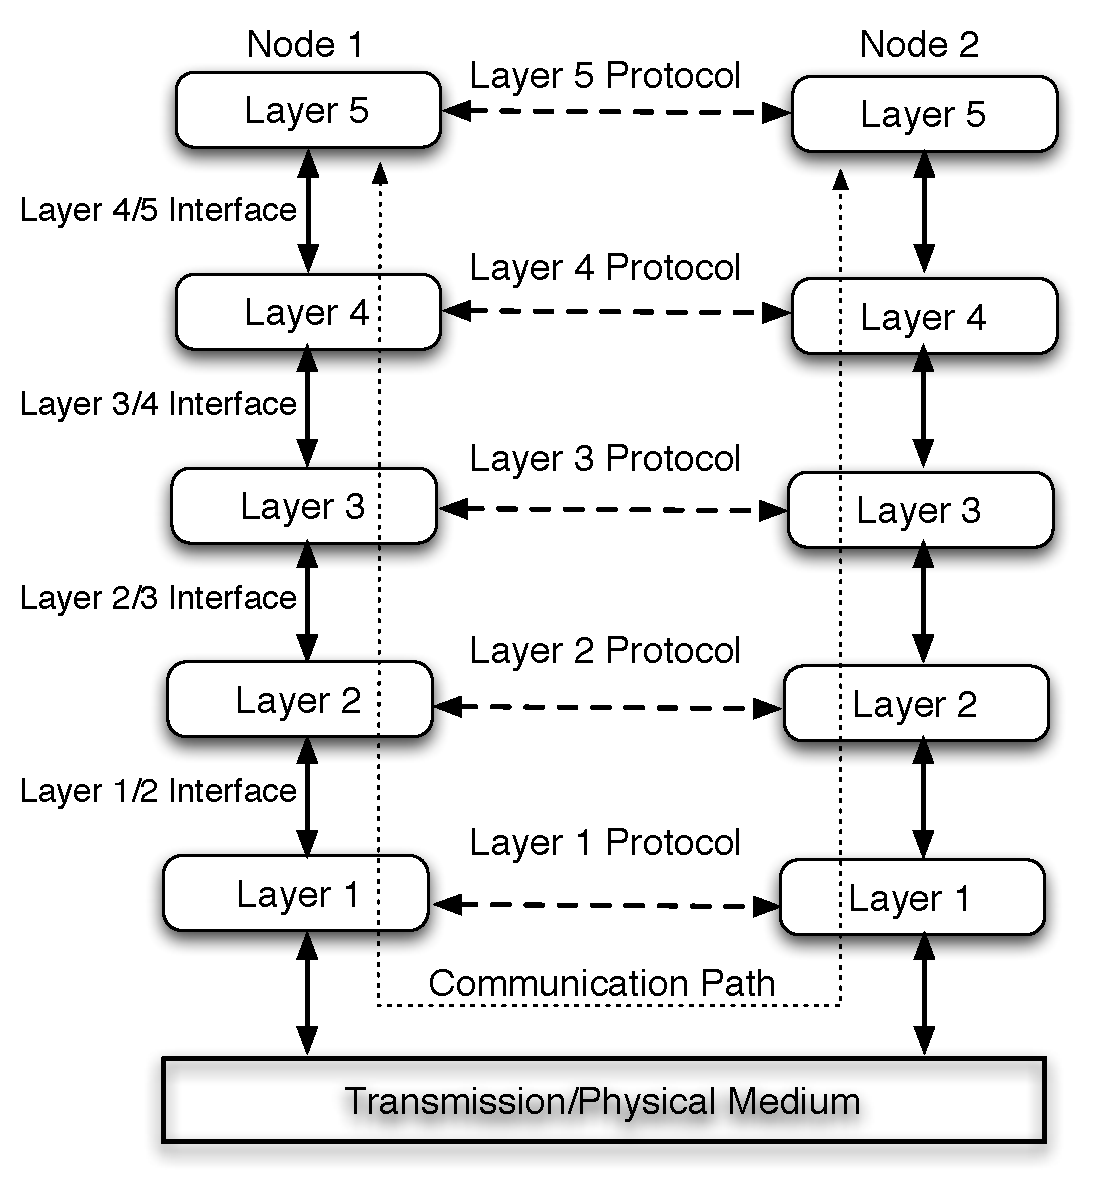
\includegraphics[scale=0.3]{RefModel}}                
  \subfloat[The OSI Model]{\label{fig:osimodel}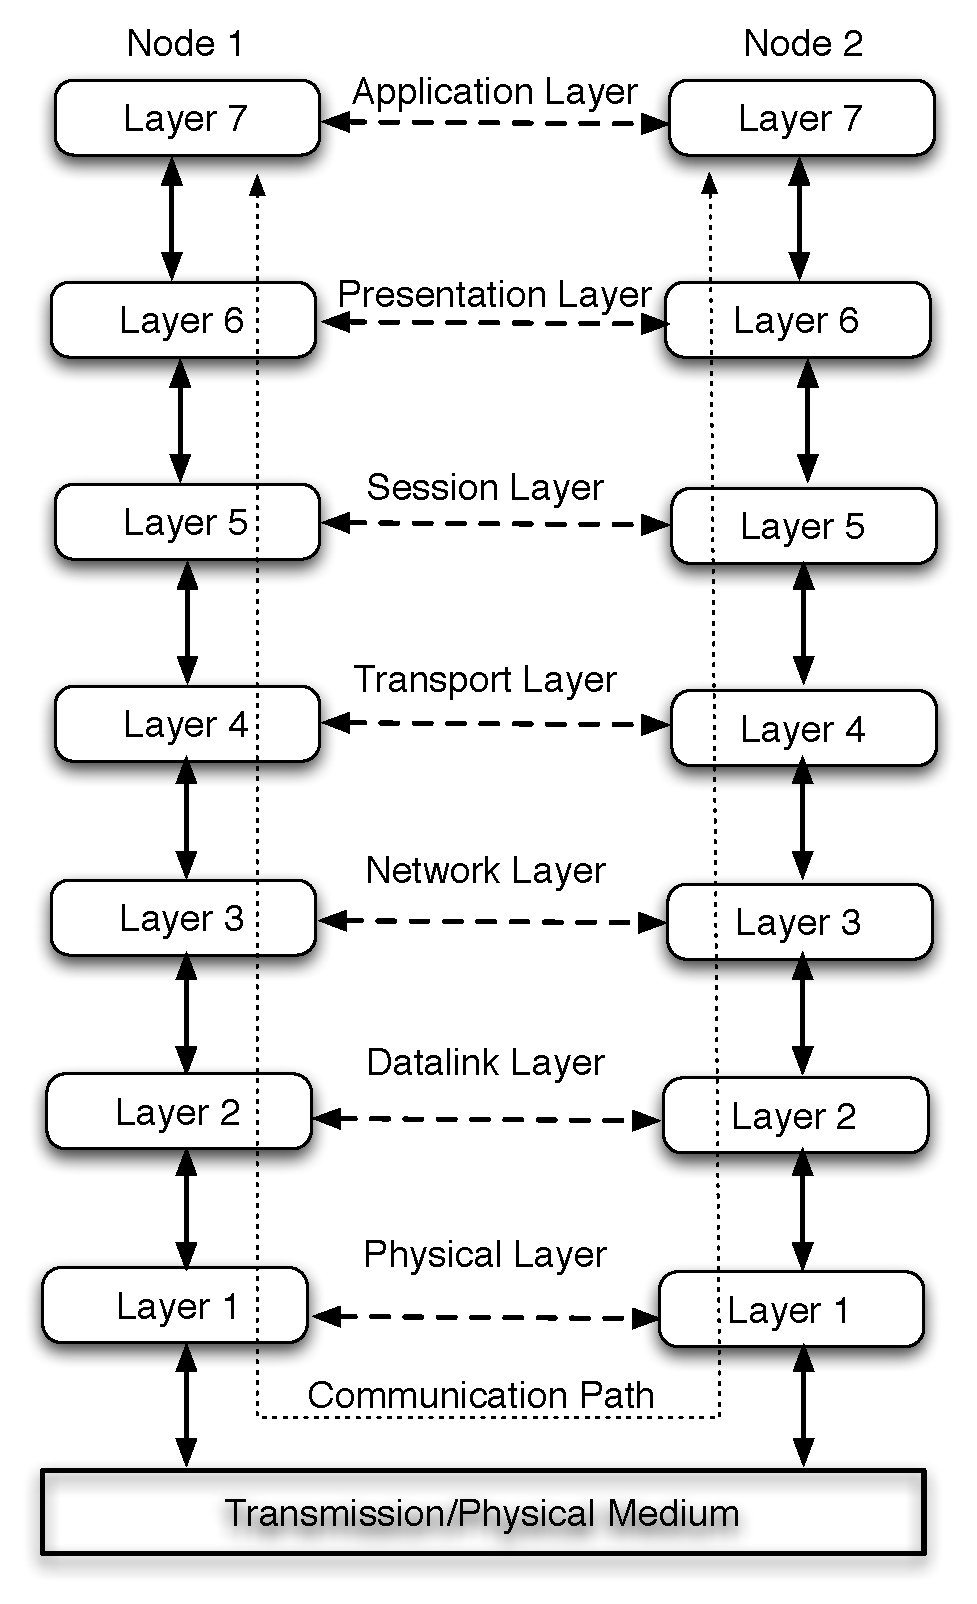
\includegraphics[scale=0.3]{OSIModel}}
  \caption{Inter-networking models}
  \label{fig:refmodels}
\end{figure}


%% Subfigure the refmodel and the osi model.
%ifigure{referencemodel}{0.45}{Reference Model (a) and OSI Model (b)}{fig:refmodel}

Figure \ref{fig:refmodels} depicts the layers, protocols and interfaces used to communicate between two nodes. Horizontal lines depict logical communication path, as no actual physical communication occurs horizontally, but rather physical communication occurs as shown by the dotted line, ie. via all the layers. 

In the next subsections, we will present two models; the OSI and the TCP/IP models. While the OSI model is general and the features addressed by each layer are still important, it is rarely used because of the bad timing of the standard ratification and its complexity. However, it is still the theoretical reference model for networks. On the other hand, the TCP/IP protocols are widely used, but the model is particular, and does not always provide a clear separation of interfaces and protocols.                                                       
                     

\subsubsection{The OSI Model}

The Open Systems Interconnection (OSI) reference model was originally developed by the International Standards Organization in an effort to standardize the protocols used in the model. Figure \ref{fig:osimodel}, shows the seven layers which make up the OSI stack. 

%\ifigure{OSI}{1}{The OSI Model.}{fig:osi}

Each layer in the OSI model performs a well defined function, and the boundaries are chosen to minimize the amount of information which has to be exchanged across the interfaces. 

We will now present the function of each layer:

\begin{enumerate}


 \item \textit{The Application Layer} is the layer which is closest to the user. Essentially this means that both this layer and the user interact with the software application.
 
 %HTTP (Hyper Text Transfer Protocol) for world wide web surfing, FTP (File Transfer protocol) for file transfer, SMTP (Simple Mail Transfer Protocol) for electronic mail, etc. Note that the protocols cited here 

 \item \textit{The Presentation Layer}, contrarily to the other lower level layers which are designed to shift bits around reliably, attempts to add syntax and semantics to to the information. It does this by providing function to operations that are performed often. 

 \item \textit{The Session Layer} enables users to establish sessions between themselves. For example, it would be used to login to a remote system or transfer a large document.
 
 \item \textit{The Transport Layer} has the basic role of obtaining data from the above session layer and splitting it up into smaller data units. These data units are then passed to the underlying network layer and the transport layer then makes sure the data arrives correctly at the other end.

 \item \textit{The Network Layer} handles and controls all the operations concerning a subnet. A particular issue is how a packet is routed from its source to its destination. These routes can either be determined statically or allocated dynamically. In this thesis we discuss different algorithms which are implemented in this layer.

 \item \textit{The Data Link Layer} has the task of obtaining the raw data from the physical layer and turning it into an input stream that seems error-free. This is accomplished by imposing that the sender split up the data into frames and transmit them sequentially. 


 \item \textit{The Physical Layer} is responsible for transmitting the raw bits over the physical medium. It is responsible for the actual translation of bits into electrical voltages or optical levels and vice versa.

\end{enumerate}


\subsubsection{The TCP/IP Model}

TCP/IP was designed for the ARPANET which was a project sponsored by the US Department of Defense (DoD). TCP/IP was built with a high degree of resiliency due to the fact that the DoD could have its installation attacked at any moment, and therefore wanted to keep communications alive as long as the end-hosts were still alive. The TCP/IP reference model, shown in Figure \ref{fig:tcpip}, was first defined by Cerf et al. \cite{CerfKahn}, and consists of four layers which we are going to detail below:

\ifigure{TCPModel}{0.7}{The TCP/IP Model}{fig:tcpip}

\begin{enumerate}

 \item \textit{The Application Layer} contains the same high level protocols described for the OSI application layer. The protocols used at this layer are denoted as Layer 7 protocols (analogy with the OSI layers), even if the TCP/IP stack only has four layers (five, depending how you consider the Host-to-Network 
Layer).

 \item \textit{The Transport Layer} provides the same functionality described by the OSI Transport layer, and its protocols are frequently denoted as Layer 4 protocols. Two end-to-end protocols are defined by the model: TCP (Transport Control Protocol) and UDP (User Datagram Protocol). While TCP is connection-oriented and provides a reliable (error free) end-to-end communication, UDP is a connectionless protocol which does not provide any guarantee on the integrity of the transmitted data. However, UDP is lightweight compared with TCP and also provides multicast capabilities (i.e. one-to-many transmission).


 \item \textit{The Internet Layer} defines the IP (Internet Protocol) protocol and packet format. This protocol is designed to deliver the IP packets over a network with multiple paths. As packets from the same conversation may follow different routes, experiencing different delays, there is no guarantee for preserving the order of IP packets. As the IP protocol provides functionality similar with that of the OSI network layer, it is often denoted as a Layer 3 protocol.


 \item \textit{The Host-to-Network Layer} is not precisely defined in the TCP/IP model except to state that the host must connect to the physical medium in order to send IP packets. The protocol, commonly, found here is the Medium Access Control Protocol, which provides addressing and medium access control mechanisms that make it possible for several hosts to communicate within a network.

\end{enumerate}


\subsection{Foundations of Ethernet.}

Ethernet is a technology which spans layers one and two of the OSI model, namely the physical layer and the datalink layer. Actually, the datalink layer has never changed since the introduction of Ethernet. The real beginning to Ethernet took place on the island of Hawaii in the early 1970s with a system named the ALOHA developed by the University of Hawaii \cite{aloha}. This system was constructed to allow radio communications between distant machines scattered over the island and a central IBM mainframe.

The ALOHA system allowed for a data rate of 9600 bits per second with fixed size frames transmitted sequentially. The mainframe would use a separate channel to convey acknowledgements of a successful transmission to sending hosts. If a terminal did not receive an acknowledgement after a fixed amount of time, it would timeout. Upon a timeout, the sending station would wait a random amount of time and attempt to retransmit. If two stations attempted to transmit simultaneously, the data arriving at the mainframe would appear corrupted due to the overlapping communications from the source stations. Such an event was referred to as a \textit{collision} causing both data packets to be lost and therefore neither station would receive an acknowledgement from the mainframe. The \textit{collision} and timeout mechanisms resulted in poor performance by the ALOHA protocol, only about 18\% of the bandwidth was ever usable \cite{Tanenbaum}.

In 1973, a researcher named Robert Metcalfe in Xerox's research laboratory in Palo Alto developed an improved version of the ALOHA system. This system, named Ethernet (Figure \ref{fig:ethernet}), was designed to interconnect computers in the laboratory. Ethernet was named after \textit{luminiferous ether}, which was thought to be the universal transmission medium for light at the end of the 19th century.

\ifigure{ethernet}{0.7}{The concept of Ethernet, as drawn originally by Bob Metcalfe.}{fig:ethernet}

With Ethernet came a new transmission medium, a thick yellow coaxial cable. Still the idea was the same as ALOHA, as the coaxial cable was the shared medium. Ethernet did not have a control channel as ALOHA did, so Metcalfe devised the Carrier Sense Multiple Access with Collision Detection (CSMA/CD) protocol \cite{Tanenbaum}, in order to better make use of the available bandwidth offered by this cable. 

\ifigure{CSMA}{0.6}{A simplified algorithm sketch for CSMA/CD}{fig:CSMA}

Figure \ref{fig:CSMA} shows a simplified flowchart of the CSMA/CD algorithm. Initially, a station must listen on the shared medium before taking a decision to transmit, as it can only transmit when the medium is free, otherwise it will cause a collision. Due to the propagation delay imposed by the shared medium, two stations may consider that the medium is free and start their transmission, thereby inadvertently causing a collision. The stations detect this collision and stop their transmissions immediately and wait a random amount of time before attempting a retransmission. The interval in which a collision may happen is referred  to as the collision window.

The maximal collision window is double the propagation time between the two ends of the network. In order for the collision mechanism to work correctly, the transmission time for the smallest frame has to be greater or equal to the collision window, if it is less then we obtain what is known as a collision fragment. It is therefore clear that a small collision window associated with the transmission of large frames would yield the maximum efficiency of the transmission medium. The Ethernet standard, however, defines the smallest and largest frame sizes possible. This in turn determines the theoretical efficiency of the network transmission, while real networks have more overhead as shown in \cite{EtherCapa}.

The Ethernet developed by Metcalfe and Xerox was so successful that Xerox, DEC and Intel drew up a standard for it which later became the base for IEEE 802.3 \cite{IEEE802.3, EtherGuide}. The transmission rate was set to 10 Mbps, the maximum and minimum frame sizes where set to 1518 and 64 bytes respectively. The official denomination 10BASE5 was adopted (10 Mbps data rate, base band transmission with network segments of 500 meters maximum). The shared medium was used for both directions thereby creating a half duplex network. In order to increase the maximum size of the network, devices called repeaters were introduced, which would clean and amplify the signal. 

\ifigure{EtherFrame}{0.6}{Structure of an 802.3 Ethernet Frame.}{fig:Ethernet}

The Ethernet IEEE standard \cite{IEEE802.3} defined the structure of the frame as shown in Figure \ref{fig:Ethernet}. The frame starts with a preamble, which is a special pattern allowing the receiver clock to synchronize with the incoming stream. The preamble is followed by the \textit{Start of Frame Delimiter (SFD)} which indicates the  immediate arrival of the frame. The source and destination fields are numbers which uniquely identify a device connected to the Ethernet network, although the destination field can contain special numbers that indicate that this communication is either multicast or broadcast. The length field is used to communicate the amount of data in the payload if it is less than 1500 otherwise this field is used to give information to higher layer on how to interpret the payload. If the payload carried is less than 46 bytes then it is padded with zeros in order to reach the minimum length of an Ethernet frame of 64 bytes. The \textit{Cyclic Redundancy Check (CRC)} enables the receiver of the frame to determine if the frame was corrupted during transmission. Every frame is followed by an idle period of 96 bit times, which indicates the \textit{End of Frame Delimiter (EFD)}.

Essentially, Ethernet was a broadcast communication protocol as all network members are listening on the cable at the same time. To this end, the IEEE standard introduced a special broadcast address (0xFFFFFFFFFFFF) to take advantage of this natural feature of Ethernet. A frame sent out with this destination address would be processed by all stations on the network. Another special group of addresses, which all have their first bit equal to 1, were used for multicast. Multicast frames where only processed by a subset of stations on the network.

As the popularity of Ethernet networks grew, and the number of stations exchanging data grew as well, it became apparent that CSMA/CD's limitations on the size of the network were a constraint. As traffic on the network increased, a phenomenon called \textit{network congestion} appeared which caused the useful throughput to drop significantly below what was theoretically expected. Protocols of higher levels which included their own congestion control mechanism, for example TCP \cite{RFC793}, caused further degradation of transfer rate as the number of stations increased. 

\ifigure{bridge}{0.5}{A bridged Ethernet network.}{fig:bridge}

The Ethernet bridge was introduced by IEEE in 1990 with the IEEE 802.1D standard \cite{IEEE802.1D}. Bridges have the feature that traffic local to a collision domain are not passed over it, shown in Figure \ref{fig:bridge}. If the network was well designed most of the traffic remained local to a collision domain, thereby increasing the useful bandwidth available on the two networks as opposed to a network with a single large collision domain.

\subsection{Evolution of Ethernet - The fast and the faster.}

In the same year as the introduction of the network bridge came IEEE 802.3i \cite{IEEE802.3i} which presented a new type of media for Ethernet Transmission: the Unshielded Twisted Pair cable (UTP). The cable enabled full duplex transmission and changed the topology of networks from a shared bus to a star. Devices were placed around a hub or a switch which was at the center of the network.

A hub is a special type of Ethernet repeater, it is in fact just a collapsed segment. While its earliest version consisted of only two ports that linked two Ethernet segments together, it quickly became possible to obtain hubs with many ports. It provided no extra functionality over the shared coaxial cable and therefore the network was still viewed as a single collision domain. Moreover, transmissions were still limited to half duplex and limited to 10 Mbps. 

A major development in Ethernet Networks was the introduction of the switch. A switch is capable of connecting any of its ports to any other one for a brief instant via rapid configuration changes as shown in Figure \ref{fig:switch}. This enabled full duplex communications and therefore practically doubled the bandwidth available on the network.  For a  network switch of N ports the number of concurrent conversations is $\frac{N}{2}$. If the internal speed of the switch fabric is sufficient to service all ports concurrently it is said to be non-blocking. A blocking switch can still handle conversations on all ports provided that the total bandwidth does not exceed its internal capacity. At that point it is said to be oversubscribed.

\ifigure{switch}{0.5}{A switched Ethernet network.}{fig:switch}

Nowadays, Ethernet networks are built using switches. A switches internal fabric does not necessarily provide enough bandwidth to satisfy any configuration. In the situation where the incoming traffic surpasses the available internal bandwidth the switch is said to be oversubscribed. This is common practice amongst network manufacturers in order to provide relatively inexpensive solutions to customers who do not need the full bandwidth.

Fiber optics were standardized in IEEE 802.3j \cite{IEEE802.3j} in 1993. Later in 1995, transmission speed was increased to 100 Mbps in IEEE 802.3u \cite{IEEE802.3u}. Finally, in 1998, Gigabit Ethernet was introduced in IEEE 802.3z \cite{IEEE802.3z}. More recently, in 2002, 10 Gbps was introduced.

Arguably, during the first decade of Ethernet there were other technologies that provided much better quality services. For example, Token Ring \cite{IEEE802.5} which provided a collision-free protocol and more bandwidth than the original Ethernet. The Asynchronous Transmit Mode (ATM) was able to provide guarantees on the bandwidth that could be shared between different types of traffic, whereas Ethernet has no such guarantee and can only be considered as 'best effort'. These technologies proved themselves to be too expensive and much more complicated than Ethernet.

As stated earlier, Ethernet is mainly a technology located at layer one and two of the OSI model, which has the modest goal of, essentially, moving frames from one wire to another. As Ethernet networks grow, it becomes more complicated to transport packets from their source to destination as there may be intermediary devices and several possible routes between them. This is what the Network Layer (Layer 3) and more precisely network routing is responsible for. 

\section{High Performance Networks - InfiniBand}

Before moving to routing techniques, we are going to detail an alternative communication technology, named InfiniBand, as its structure resembles modern Ethernet and its control structure is similar to OpenFlow (see \ref{sect:OPFW}). Therefore, we believe that the novel congestion protocols could be adapted to function in an InfiniBand network.

%Industry standard for inter-server I/O
	%established by a consortium of about 180 companies under the InfiniBand Trade Association (IBTA)
	% Membership is open to Universities and Research labs.   
	%Designed to provide higher levels of scalability, availability, performance and reliability.
	% The InifiniBand Architecture (IBA) is the spec resulting from the IBTA [1,2], it is 1500 pages long...
	
Infiniband has established itself as the industry standard for inter-server I/O. It was established by a consortium of about 180 companies under the InfiniBand Trade Association (IBTA). Membership to the IBTA is open to universities and research labs. Infiniband was designed to provide high levels of scalability, availability, performance and reliability. Achieving this goal does not come easy, the InfiniBand Architecture (IBA) has a 1500 page long specification \cite{InfiniBand}.


	
 %Spec so large to accomodate for:
 	%scale up and down, depending on the required solution
		%this has lead to multiple link width, multiple MTU, optional major features. To simplify all these options, IBA supports profiles containing predefined option sets.
	%encourage innovation and new inventions  
		%produced off results, ex. copper connectors defined but the length and gauge is not. Instead an attenuation (15dB) is defined.
		%the spec contains no API or registers only a set of actions expressed as verbs.
		
The length of the specification allows the IBA to scale up and down depending on the required solution for the problem. On the other hand, this has lead to the development of many options, such as multiple link widths, multiple MTU, optional major features, and many more. This has become confusing and therefore IBA supports profiles which contain predefined options in order to simplify the deployment of IBA. 

%IBA was defined due to the fact that processing power was starved by trailing I/O. 
	%This is due to that all modern computer systems employ busses.
	%These are inherently shared mediums and therefore require an arbitration algorithm which incur an overhead. 
	%On top of this, busses are memory-mapped and therefore are accessed via the CPU's store and load operations. Store don't pose much of a problem as they can overlap with computation, but load are costly as the CPU will probably need the result of the operation rather sooner than later.
	%Finally, a third reason is that busses do not deliver the level of availability or reliability required by high performance systems. Indeed, a single failed on a bus may disrupt some or all other devices attached to the bus.
	
The IBA was developed due to the fact that processing power was starved by slow I/O, mainly because modern computer still rely on buses to transport data (at least until the adoption of PCI-Express). Buses are inherently shared mediums and therefore require an arbitration algorithm to mediate access to the said bus but this comes with a significant overhead. On top of this, buses are memory-mapped and therefore are accessed via the CPU's store and load operations. A store operation does not  pose much of a problem as it can overlap with computation, but load operations are costly as the CPU will probably need the result of the operation rather sooner than later and therefore the CPU will have to wait until this information becomes available. Finally, a third reason is that busses do not deliver the level of availability or reliability required by high performance systems. Indeed, a single failed device on a bus may disrupt some or all other devices attached to the bus.


	
%To overcome limitations posed by busses
	%Infiniband defines point-to-point connections, and therefore data transfer is not bussed.
	% message semantics, command and data exchanges are done via messages and not as memory operations.
	% Like any modern communication system, IBA is a stack divided into the physical, link, network, and transport layers.
	
	

As a solution to the problems encountered by buses, IBA defines  point-to-point connections, and therefore data transfer is not bussed. Moreover it defines message semantics and therefore command and data exchanges as achieved via messages and not as memory operations. As many modern communication systems, the IBA is defined as a stack containing a physical, link, network,  and transport layer.  

	
	%Smallest functional IBA system is a subnet which can be joined together by router to form larger systems similarly to modern IP networks.
	% The subnet consists of endnodes, switches, links and a subnet manager. 

	%Switches route data from a source to a destination based on the routing tables computed either at the network's init and/or network modification.
	%The exact structure and format of the router depends entirely on the subnet manager as it is the entity responsible for maintaining the tables.
	%Subnet managers send messages to the devices they control (ie. the agents).  Each IBA system must contain at least one subnet manager that can either reside on an endnode or a switch.  The subnet manager discovers all the devices on the network and assigns them local IDs, and compute the routing tables to be loaded a each device. There has been some study of routing techniques used in IBA systems [4] as well as some extension proposals [3].
	% During operation, the subnet manager scans the network to discover additions or deletions.
	%All manger traffic is sent in-band.
 
 The smallest functional IBA system is a subnet which can be joined together by router to form larger systems in a similar manner to modern IP networks. Switches route data from a source to a destination based on the routing tables computed either at the network's initialization and/or network modification. The exact structure and format of the routing tables depends entirely on the subnet manager as it is the entity responsible for maintaining the tables. Subnet managers send messages to the devices they control (ie. the agents).  Each IBA system must contain at least one subnet manager that can either reside on an endnode or a switch.  The subnet manager discovers all the devices on the network and assigns them local IDs, and computes the routing tables to be loaded a each device. There has been some study of routing techniques used in IBA systems \cite{IBACurrentRoute} as well as some extension proposals \cite{IBAExtensions}.
 
 The architecture of an IBA is similar to the solutions developed in this document to construct network protocols. Therefore, it is the author's belief that even though the implementation presented in this thesis employed Ethernet, that the same approach could be used in IBA systems. Indeed, a central aspect of an IBA system is the subnet controller which is quite similar to an OpenFlow controller (see Section \ref{sect:OPFW}), which is used to control Ethernet device behavior. 	    

%[1,2] Infiniband spec architecture volumes 1 and 2
% [3] Improving InfiniBand Routing through Multiple Virtual Networks -- extension
% [4] Evaluation of Routing Algorithms for InfiniBand Networks -- study

\section{Routing - Where to next?}

At the end of the previous section we discussed primarily Layer 2 networks, which only provide means for transport frames from wire to wire over an Ethernet hub or switch. Layer 3, the network layer, is concerned with transporting packets from the source to their final destination \cite{DataNetworks}. This process, called \textit{routing}, achieves this goal by using devices called routers. This goal may seem simple, but the algorithms they employ are complex. Moreover, there is a variety of routing protocols which define how routers can communicate to determine the best routes to all destinations.

The origins of routing can be traced back to the late 1950s, where various shortest path algorithms where proposed by Ford \cite{Ford1956}, Bellman \cite{Bellman1958}, Floyd-Warshall \cite{WARSHALL1962} and Dijkstra \cite{DIJK}. These algorithms compute the shortest path between a source and destination pair in a graph, and they make up the core of current routing protocols implemented nowadays. Each link in a network is given a cost, and therefore the cost of a path is the sum of the constituent link costs, and trivially the shortest path is the path with the lowest cost. Since these algorithms provide remarkable simplicity and generality, they have been in use since the early days of the ARPANET \cite{ARPANET} to networks nowadays.

Routing is a complex process, which involves several independent algorithms exchanging information between themselves. There are a several reasons for this complexity:

\begin{itemize}
 \item Routing requires all the network nodes to coordinate to offer a coherent routing strategy.
 \item Routing must be capable of surviving link and node failures, this requires the algorithms to provide alternative paths and therefore to keep their routing databases up-to-date.
 \item In order to achieve high performance, a routing strategy may be required to modify its routes as areas of the network become congested.
\end{itemize}

\subsection{Some Issues in Routing}

%Routing performes two main functions, the first is the selection of routes for each source-destination pair and the second is the actual delivery of the packets. The second function is simple to implement with the help of routing tables

Routing affects mainly two performance metrics, the first is \textit{Throughput} (Quantity of Service) and the second is \textit{average packet delay} (Quality of Service) \cite{DataNetworks}. These metrics are determined by the flow control mechanism provided by the Transport Layer as shown by Figure \ref{fig:RouteFlowControl}. 

\ifigure{RouteFlow}{0.6}{Interaction between Transport and Network Layer}{fig:RouteFlowControl}
                
When the network is lightly loaded we can easily say that,

\begin{equation}
  Throughput = Offered Load
  \label{eq:THEQOF}
\end{equation}

As network load increases the flow control scheme will reject some traffic, due to congestion. We therefore have Equation \ref{eq:THEQOFR},

\begin{equation}
  Throughput = Offered Load - Rejected Load
  \label{eq:THEQOFR}
\end{equation}

Traffic within the network will also receive an extra delay due to time required for the routing scheme to select the appropriate path. This (and other indirect factors resulting from the rejected load) will significantly affect the throughput as flow control schemes attempt to strike a balance between throughput and delay. Therefore, we can say that the more the routing scheme keeps delays low, the more the flow control scheme will allow traffic on the network.

%as illustrated in Figure \ref{fig:GoodBadRouter}

%\ifigure{GoodBadRouting}{0.7}{Delay vs. Throughput curves - The good and bad Routing.}{fig:GoodBadRouter}

%\begin{figure}[htbp!]
%\begin{center}
%
%\begin{tikzpicture}[scale=1.0, domain=0:9.8]
%    \draw[very thin,color=gray,step=.5cm] (-0.1,-0.1) grid (10.2,10.2);
%    \draw[->] (-0.2,1) -- (10.2,1) node[below = 28pt, left=3pt] {$Load$};
%    \draw[->] (1,-0.2) -- (1,10.2) node[left = 28pt, below=5pt] {$\rotatebox{90}{Delay}$};
%    \foreach \x/\xtext in {10/1}
%      \draw[shift={(\x,1)}] (0pt,2pt) -- (0pt,-2pt) node[below] {$\xtext$};
%    \foreach \y/\ytext in {10/1}
%    \draw[shift={(0,\y)}] (2pt,0pt) -- (-2pt,0pt) node[left] {$\ytext$};
%
%%MODIFIED BY HAND
%
%    \draw[color=black] plot[id=loggood] function{(1/(1-((x/10)**5)))}
%    	node[above=1pt] {Good routing};
%    \draw[color=black] plot[id=logbad] function{(1/(1-((x/10)**3)))}
%      node[left=10pt] {Bad routing};
%
%     
%%     \draw[color=black] plot[id=exp2] function{4*(1 - 500**(-x/4))}
%\end{tikzpicture}
%
%\end{center}
%\caption{Delay vs. Load curves - The good and bad Routing.}
%\label{fig:GoodBadRouter}
%\end{figure}

\subsection{Properties of Routing Algorithms}

Before entering into the classification of routing algorithms let us first describe some desirable properties for routing  
algorithms: correctness, simplicity, robustness, stability, fairness, and optimality \cite{Tanenbaum}.

\begin{itemize}
 \item \textit{Simplicity} and \textit{Correctness} are trivial. All routing protocols should provide a simple solution to the routing problem, and maybe more importantly they should be correct.
 \item \textit{Robustness} - When a routing algorithm is brought online, it may be expected to run for many years. Therefore, it must be able to withstand failures, changes in topology and traffic patterns.
 \item \textit{Stability} is one of the most fundamental aspect of a routing algorithm simply because an algorithm which does not converge to some equilibrium could cause unpredictable network results.
 \item \textit{Fairness} and \textit{Optimality} - While they are enormously desirable properties, they are often opposed. As shown in Figure \ref{fig:fairvsopti}, suppose the horizontal links between A and A', B and B', and C and C' are saturated. In order to maximize the total flow, traffic between X and X' should be virtually non existent, but from X and X' point of view this is unfair. Therefore there is a tradeoff between fairness and optimality. 
\end{itemize}

\ifigure{fairvsopti}{0.5}{Conflict between fairness and optimality.}{fig:fairvsopti}

One last important concept before we move onto the classification of routing algorithms is a statement about optimal routes regardless of topology and traffic. This is known as the \textit{Optimality Principle}. In its simplest form it states that if a router B lies on the optimal path between routers A and C, then the optimal path between B and C falls on the same route. The major consequence of this principle is that all the routes from any source to a given destination comprise a tree rooted at the destination. This tree is called a \textit{Sink Tree}.

\section{Classification and the Evolution of Routing Algorithms.}

In this section we will attempt to classify routing algorithms while presenting their evolution from the original graph algorithms. We will not enter into the details of the graph algorithms, for more information see Section \ref{sect:GraphAlgo}.  Two classes are commonly used to group routing algorithms: \textit{Static} and \textit{Adaptive}. In static algorithms, all routes are computed off-line and this configuration is then downloaded to the routers. This is sometimes referred to as \textit{Source Routing}. Adaptive algorithms react to changes in topology and network state (such as congestion, delay, or other metrics), these protocols are the most common in packet switched networks \cite{DataNetworks}. Another class of algorithms we will discuss are called \textit{Optimal Routing} Algorithms. Although they have never had a real world implementation, they have an influence on multipath routing algorithms which will be discussed in Chapter \ref{chap:multipath}.
 
\subsection{Static Algorithms}
\label{sect:static}
The most basic static routing algorithm is to compute all the possible source-destination shortest paths off-line using a Shortest path algorithm \cite{DIJK, WARSHALL1962, Bellman1958}. Then, use the output of this computation and install static routes at each router in the network. The details of these algorithms will be given in Section \ref{sect:GraphAlgo}.

Another static algorithm is \textit{Flooding}, where each incoming packet is sent on every outgoing line except the one it arrived on. Clearly, this algorithm generates many duplicate packets, and it can be shown that an infinite number of duplicates will persist in the network. To avoid these duplicates, each packet contains a hop count field which is incremented at each router. When the counter reaches some predefined limit the packet is dropped. Flooding is actually used in current protocols, such as OSPF \cite{OSPF}, in order to advertise a routers connections.

The two previous algorithms only consider topology. \textit{Flow-based routing} considers both topology and network load. The assumption here is that the capacities and the average load for each link in the network is known. If these values are known and so is the topology, it is possible to compute the mean delay from queuing theory. Finally, from the mean delay for each link it is then simple to calculate the mean packet delay for the entire subnet. 

\subsection{Adaptive Algorithms}

Nowadays networks mainly use dynamic routing algorithms rather than static ones. The two main classes of algorithms are presented here: \textit{Distance Vector} and \textit{Link State} routing.

\subsection{Distance Vector Routing}

Distance Vector Routing algorithms function by having each router maintain its best known distance to each destination and which outgoing link to use in a routing table. Each entry is composed of the outgoing line and the metric estimate for each destination.  These tables are then exchanged with each of the neighboring routers. The metric used to compute the distance may either be the number of hops, delay, or the number of packets queued along the path (queue depth). The local router knows its distance to all its neighbors, if the metric is hops then its distance is one hop. If the metric is queue depth, then the router simply measures it. Otherwise if the metric is delay, the router can send a special echo packet in order to measure the delay. 

\ifigure{DVEvo}{0.7}{Evolution of Distance Vector Algorithms}{fig:DVEvo}

As an illustration of Distance Vector algorithms, assume that the metric is hop count and therefore the router knows that all its direct neighbors are within one hop. Periodically, every router sends its hop counts (exchange vector) for each destination to each of its neighbors, while also receiving one from every neighbor. Consider that router Y receives an exchange vector from router A containing the hop count $A_B$, which is the hop count from router A to B. If Y knows its hop count to A, denoted $Y_A$, then it can conclude that B is $Y_A + A_B$ hops away, and update its routing table accordingly. If this is done for all neighbors, a router will have an estimate of distances to each other router in the network.

Distance Vector Algorithms are sometimes called distributed Bellman-Ford routing algorithms or the Ford-Fulkerson algorithm, because of the researchers who developed it \cite{Bellman1958, Ford1956}. Other implementations of distance vector algorithms include RIP \cite{RIP} and the original routing algorithm of the ARPANET \cite{ARPAORIG} as shown in Figure \ref{fig:DVEvo}. Distance Vector algorithms still exist in some current routing algorithms as shown in \textit{EIGRP} \cite{EIGRP}, as shown in Figure \ref{fig:CurrEvo}.

%These protocols lead us to some of the implemented protocols which will be discussed in Section \ref{sect:evolutioncurrent}.

While Distance vector works very well in theory and reacts quasi perfectly when a newer and shorter route appears, there are situations where these algorithms can take a a very long or even infinite amount of time to converge. Consider the situation when a router X, only knows of a very long path to Z. If now a router Y tells X that it knows of a shorter route to Z, X will directly change its forwarding table to reflect this situation. This situation describes the normal and optimal operation of a Distance Vector algorithm.  

\begin{table}[!htbp]
  \begin{center}
  \subfloat[A good news situation]{\label{tab:countinfgood}
    \begin{tabular}{| c | c | c | c | c || c |}
      \hline
      A & B & C & D & E &  \\
      \hline
	0 & $\infty$ & $\infty$ & $\infty$ & $\infty$ & initial situation \\
	0 &  1 & $\infty$ & $\infty$ & $\infty$ & one exchange \\
        0 &  1 & 2 & $\infty$ & $\infty$ & two exchange\\
	0 &  1 & 2 & 3 & $\infty$ & three exchanges \\
	0 &  1 & 2 & 3 & 4 & four exchanges \\
	\hline
    \end{tabular}
    }
\vspace{0.5cm}
\\
%(a) A good news situation.
%\vspace{1cm}
%\\
\subfloat[A bad news situation]{\label{tab:countinfbad}
  \begin{tabular}{| c | c | c | c | c || c |}
      \hline
      A & B & C & D & E &  \\
      \hline
	 & 1 & 2 & 3 & 4 & initial situation \\
	 &  3 & 2 & 3 & 4 & one exchange \\
         &  3 & 4 & 3 & 4 & two exchange\\
	 &  5 & 4 & 5 & 3 & three exchanges \\
	 &  5 & 6 & 6 & 6 & four exchanges \\
	 \multicolumn{6}{c}{\rotatebox{90}{\dots}} \\
	& $\infty$ & $\infty$ & $\infty$ & $\infty$ &  \\
      \hline
    \end{tabular}}
%\vspace{0.5cm}
%\\
  %(b) A bad news situation

  \caption{Count-to-infinity problem.}
   \label{tab:countinf}
  \end{center}
\end{table}

Consider a topology where for the simplicity of argument, all the routers (A through E) are arranged in a line. Figure \ref{tab:countinf} illustrates the distance tables at each router to A. Figure \ref{tab:countinfgood} depicts the situation when all the routers are up and functioning correctly. Figure \ref{tab:countinfbad} shows the situation when A has suddenly gone down for some reason (link failure or broken router). At the first exchange, router B does not receive a message from A, but C tells B that it has a path to A of length 2. The problem here is that B does not know that the path advertised by C passes through itself. Therefore B thinks it can reach A via C with a length of 3. Next C notices that all the routers around have a path to A with length 3, and therefore it must update its table. By doing so it causes the same sequence of messages to occur again as shown in Figure \ref{tab:countinfbad}. Therefore all the routers never cease to update their tables, and will keep increasing their path length to A ad eternum. This issue is known as the \textit{count-to-infinity} problem.

%Bouncing effect? Maybe...

In 1975, Cegrell introduced the concept of \textit{Split Horizon} \cite{Cegrell75} to counter the effect of the count-to-infinity problem. Split horizon operates on a very simple premise, if a node A is routing traffic to a destination X via node B, it makes no sense for B to try to route to X via A. Therefore it is useless for A to announce to B that X is close to A. Split Horizon is elegant as it only involves a small change to the routing algorithm. Indeed, instead of a router always broadcasting all its routes on all its links, it simply modifies the exchange message on the the links that some destinations are actually routed through. 

%Split horizon with poisonous reverse? Maybe...

Unfortunately, split horizon does not solve the problem entirely. Consider two connected routers X and Y who both connect to T via Z. Suppose that initially both X and Y have a distance 2 to T, and Z has a distance 1. If the link between Z and T goes down for some reason, both routers X and Y report that they cannot get to T and Z reports that T is unreachable. Unfortunately in the meantime, X and Y both exchange their routing information where they have a route to T. Causing X and Y to think they can reach T via Y and X respectively, with length 3. After this, for every exchange they increment their length to T by one and therefore we are back to the count-to-infinity problem. This is known as a three-way loop.




\subsubsection{Some important Algorithms}
\label{sect:DUAL}
In this section we will discuss some algorithms, developed by Garcia-Luna-Aceves, which had an influence on some of the multipath algorithms discussed in Chapter \ref{chap:multipath}.

In early 1993, Garcia-Luna-Aceves proposed a family of innovative routing algorithms, named \textit{Diffusing Update Algorithms} (DUAL) \cite{DUAL}, which computed shortest paths using diffusing computations based on the idea presented in \cite{DijkstraTerm}. Diffusing computations is a computation that takes place over a set of networked machines. Dijkstra proposed method \cite{DijkstraTerm}  for detecting the termination of the computation. DUAL provides loop-free operation at every instant throughout a route computation. This allows routers involved in a topology change to synchronize at the same time, while not involving routers that are unaffected by the change. DUAL is currently used by \textit{EIGRP} \cite{EIGRP}, which is a Cisco proprietary routing protocol.

A few years later in 1997, Garcia-Luna-Aceves presented an algorithm for \textit{Loop-free Path-finding Routing} named LPA \cite{LPA}. This algorithm eliminates the temporary formation of routing table loops during a topology change more efficiently than DUAL. A routing table loop is a path which is specified by the routers' routing tables at a specific time (usually during a topology change), which causes a packet to visit the same node more than once before reaching its destination. 

Finally, later that same year, Garcia-Luna-Aceves presented a more \textit{Efficient Distance Vector Algorithm} (EDVA) \cite{EDVA}. EDVA uses the enhancements of the two previously described algorithms to reduce the convergence time and the number of control packets needed by the routing algorithm. As we will see later, EDVA has had some influence on multipath routing algorithms. 
%Discuss DUAL, LPA, EDVA important because DUAL and EDVA influences some multipath algos.

\ifigure{CurrEvo}{0.5}{Evolution of Implemented Routing Algorithms}{fig:CurrEvo}

\subsection{Link State Routing}

%Link State algorithms are the protocols which currently make up the most of Internet, therefore in this section will focus on the improvements over Distance Vector that Link State brings and defer their evolution to Section \ref{sect:evolutioncurrent}.

Link State algorithms came about as a replacement to Distance Vector algorithms and provided the major improvement of being free of the count-to-infinity problem. While this improvement is highly desirable, it came at a price, Link State algorithms need to maintain a complete and up-to-date vision of the network topology at every participating node. In order to achieve this goal, Link State algorithms must initially discover all their neighbors. Then, they must measure the cost (in terms of hops or delay) to each discovered neighbor. Next, this discovery must be advertised to all routers in the network, as we will see this is achieved via Link State packets. Only once all this information is gathered can the algorithm compute the shortest path to every other router using Dijkstra's Shortest paths algorithm \cite{DIJK}.

Link State algorithms provide several advantages over Distance Vector algorithms as is shown below:

\begin{itemize}
 \item \textbf{Loopless and Fast Convergence} - As we have seen with Distance Vector schemes, the number of steps required to achieve convergence can be large and even sometimes infinite. Link State solves this by distributing information rapidly via a flooding protocol, and then performing a computation which is local to every router. Immediately after the computations all the routes are guaranteed to be valid and loopless.
 \item \textbf{Multiple Metrics} - Distance vector schemes do not cope well with multiple metrics. Indeed, if a single metric can have several orders of magnitude in variation, introducing others will probably cause the algorithm to converge very slowly as the solution space is expanded. Whereas Link State algorithms perform their computation with full topology knowledge, there can be as many metrics as desired.
 \item \textbf{Multiple Paths} - Nowadays, complex networks provide paths which are either identical or very similar to the shortest path. Distance Vector algorithms cannot support multiple paths in their current form because the routing table can only accommodate one entry per destination \cite{Huitema}. In Link State, a simple modification to shortest path computation can be added and this will provide us with a list of candidate equal cost paths for a given destination. Thereby, this has the potential for increasing the overall performance of the network.
\end{itemize}

Neighbor discovery is achieved by sending specially crafted \textit{HELLO} packets on each of the router's outgoing lines. Any router receiving such a packet must respond immediately indicating its identity. This introduces an, albeit minor, constraint to Link State protocols which is that router identities must be unique. A line's cost can easily be estimated by sending a \textit{ECHO} packet. As with the \textit{HELLO} packet, once a router receives a \textit{ECHO} packet it sends it back immediately. This provides an estimate for the round trip time on a given line, which is then divided by two to obtain the line delay.

Once the information described above has been collected, the router builds the Link State packets. The distribution of the link state packets must be achieved reliably in order to guarantee that each router has the same view of the network. This distribution is achieved via a flooding algorithm similar to the one described in Section \ref{sect:static}.

Nowadays, most of the Internets routes are governed by OSPF \cite{OSPF}. OSPF grew from an early link state algorithm which was designed to replace RIP \cite{RIP} in the ARPANET \cite{ARPAROUTE}. It took over most of the functionalities developed in IS-IS \cite{RFC3787}. This evolution is shown in Figure \ref{fig:CurrEvo}.

\subsection{Optimal Routing}

Optimal Routing aims at optimizing the average global delay of a network, instead of only finding a shortest path. Therefore the problem of computing optimal routes in a network can be expressed as a optimization problem (more precisely, a nonlinear multicommodity flow problem) \cite{CANTOR74}, this will be explained in more detail in Chapter \ref{chap:theory}.

 Performance and costs are usually measured by metrics like delay, maximum line utilization, packet loss rate, stability of the system, and convergence time after failures. Current routing methods used in the Internet are not optimal in terms of any of these metrics. For instance, most of the routing protocols use hop-counts, or weights (derived from metric estimates) assigned to the lines in order to derive the routing tables which obviously cannot optimize any of the metrics mentioned above. 

A direct way to improve the routing process (ie. optimize in some sense the metrics described above) is to use multiple paths between source-destination pairs. Current protocols, such as OSPF \cite{OSPF} or IS-IS \cite{RFC3787} do this in a limited sense, by splitting the load to a destination along multiple shortest paths if these exist. This is an improvement, but still it is not optimal.

\ifigure{OptEvo}{0.5}{Evolution of Optimal Routing Algorithms}{fig:OptEvo}

Optimal Routing has been researched and studied for many years. Its simplest form is Flow-Based Routing (see \ref{sect:static}) where a network is modeled by a set of nodes which are connected by links. The capacity and amount of traffic on each link is known, and using this information the total cost to transport messages is minimized.

 In 1974, Cantor and Gerla \cite{CANTOR74} modeled this problem as a optimization problem and used separation techniques to solve it. In 1977, Gallager \cite{Gallager-mindelay} proved the necessary and sufficient conditions for having a minimum-delay routing and introduced a distributed multi-path routing algorithm for this purpose that is loop-free at each iteration under the assumption that the network traffic is stationary or slowly changing. In 1999, Garcia-Luna-Aceves proposed a new algorithm, called Near-OPT \cite{NearOPT}, which constructs multiple loop-free paths, and then applies a similar method to the one proposed by Gallager. This algorithm is the basis of a multipath algorithm which will be described in Chapter \ref{chap:multipath}.
 Figure \ref{fig:OptEvo} depicts the evolution of Optimal Routing algorithms. None of these methods were used in practice due to their complexity as well as low performance of processors and low capacity of links at the time these methods were proposed.

%-- Stem from gallager-mindelay. (see survey chapter 4)

\section{Summary}

In this section, we have presented the fundamentals of networking along with a history of routing algorithms. Over time the OSI model has turned into a reference only model, while the TCP/IP model is virtually ubiquitous. Ethernet has evolved from 9600 bits per second beginnings to 10 Gbps with 100 Gbps at our doorstep.

Distance Vector algorithms have been mostly replaced by Link State ones. Primarily due to their shortcomings in terms of convergence time and their inability to support sophisticated metrics. Optimal Routing algorithms have for long been a mathematicians toy and a networks researchers dream, due to the fact that they were only implementable in a centralized manner.

In the next chapter, we will discuss the state-of-the-art in multipath routing. These algorithms attempt to reconcile the best from Link State or Distance Vector routing and Optimal routing. 

\chapter{Multipath Routing}
\begin{flushright}
 \textit{\textquotedblleft If you want to succeed you should strike out on new paths, \\ 
rather than travel the worn paths of accepted success.\textquotedblright}\\
\textit{-- J. D. Rockefeller}
\end{flushright}
\label{chap:multipath}

\ifpdf
    \graphicspath{{3-MultipathRouting/Chapter2Figs/PNG/}{3-MultipathRouting/Chapter2Figs/PDF/}{3-MultipathRouting/Chapter2Figs/}}
\else
    \graphicspath{{3-MultipathRouting/Chapter2Figs/EPS/}{3-MultipathRouting/Chapter2Figs/}}
\fi

\section{Why Multiple Paths: Some justifications}

Computer networks have grown over the past decades, this growth has lead to a rise in complexity of their topology. While increased complexity is often viewed negatively, it may be a blessing in disguise to networks because it can provide multiple paths towards a destination. If we are able to utilize these alternative paths intelligently, we can expect ta significant increease in network performance.

\ifigure{multipath}{0.5}{A complex network}{fig:ComplexNet}

Figure \ref{fig:ComplexNet} shows a complicated network consisting of multiple paths between a given source-destination pair. For example, consider source A and destination C: we have four possible paths from A to C (A-B-C, A-D-C, A-D-B-C, A,D-E-C). Most protocols nowadays, only consider a single path at any given instant. While such a decision reduces the diffculty in building correct routing tables, it comes with a major drawback: instead of using the entire capacity of the network, one will only use a relatively small fraction (in this case, only a fourth is used).

It has been proven that splitting traffic over multiple paths reduces delay while increasing he efficiency of the network \cite{ParaQueue, Huitema}. If all packets of a given communication can be assigned to one path, then we will obtain higher network throughput as several communication can occur simultaneously and lower delays in both absolute terms and delay variations. Moreover, using multiple paths solves another problem which is encountered in single paths routing: link failure. If a link fails in a multipath scenario, then the traffic can simply be rerouted via an alternative path while a recalculation occurs or the failed path is re-established contrasting with single path routing where the routing tables must be recalculated and all traffic is lost in the meantime. 

%possibly talk about congestion???

On the other hand, splitting traffic over multiple paths comes with its own problems. First, it is possible that packets on different paths encounter different path MTU (Maximum Transmission Unit) and therefore would require a router to break up packets according to the path they take, thereby negating the advantage of an advertised MTU. Second, debugging tools, such as traceroute or ping,  are made inaccurate or even incorrect due to the use multipaths. Finally, a much more serious problem, is the phenomenon of variable delays encountered by packets on different paths which cause them to arrive out of order. In many TCP (Transmission Control Protocol \cite{TCP}) implementations, out of order packets cause retransmissions which drastically reduce the performance of a network. A solution to this problem is suggested in Section \ref{sect:eqcostmulti}.

Before we continue, we must introduce the concept of \textit{flow}, which in this document is similar to the definition of a microflow in \cite{RFC2474}. 

%\newtheorem{definition}{Definition}
\begin{definition}
 A \emph{flow} is a sequence of packets which is identified by its characteristics, such as source and destination address, source and  destination port. Where characteristics could for example be same header values.
\end{definition}

There are two features which are desirable for multipath protocols:
\begin{itemize}
 \item \textbf{Minimal Disruptions} - Since multipath protocol route traffic on many paths, the probability of one path failing or removed for an arbitrary reason is much greater than in the case of single path. It is therefore desirable to minimize the number of flows affected by a link removal.
 \item \textbf{Fast Computation} - The overhead required to compute the next hop to forward a packet or flow should be small when compared with single path protocols.
\end{itemize}


Multipath routing, essentially, asks the question of how to best split network traffic on a set of paths given some cost function. This is known as a flow maximization problem and is a very difficult problem to solve. Moreover, we are not looking for a centralized solution, nor a distributed solution where routers make their own decisions, but a solution based on a feedback loop where decisions are influenced by the evolving network conditions. The centralized solution is NP-Complete, but if we retain some network paths we can solve the problem in a bounded time by assigning a price to each link of the network. The price is the first derivative of the cost function evaluated at the offered traffic level. In order to estimate the offered traffic we must first be aware of all the routing decisions taken by all routers, and therefore this makes such algorithms difficult, if not impossible, to implement in a real network. Moreover, such approaches will inevitably suffer from scalability problems and therefore convergence problems. These problems make up a very active field of research.    


\section{Multipath Routing Schemes}

As it has been shown in the previous section, single path algorithms, such as OSPF, RIP, EIGRP \cite{RIP,OSPF,EIGRP}, make inefficient use of the overall network bandwidth. In this section we present some research multiple paths algorithms whose evolution is shown in Figure \ref{fig:multipathevo}. 

\ifigure{multipathevo}{0.5}{The Evolution of multipath algorithms}{fig:multipathevo}

\subsection{Proposed Extensions to Single Path routing}

Multiple Path Algorithm (MPA) \cite{MPA} is an extension that could be added to OSPF \cite{OSPF}. MPA constructs a subset of paths in a given network which satisfy a condition for loop freeness. This algorithm introduces the notion of a \textit{viable next hop}, where initially the shortest paths are computed. A router then computes the difference between its neighbor's path length to the destination and the distance to get to its neighbor, if this distance is \textbf{less than} the distance from the router to the destination then the path is considered viable. More formally, for every neighbor N of router R the test in Equation \ref{eq:viableroute} is performed:

\begin{equation}
  D_N(R,X) - d(R,N) < D(R,X)
 \label{eq:viableroute}
\end{equation}

Where,
\begin{itemize}
 \item $D_N(R,X)$ is the distance from neighbor N to destination X
 \item $c(R,N)$ is the cost of the link between R and N
 \item $D(R,X)$ is the distance from R to X.
\end{itemize}

\ifigure{MPA}{0.7}{An example of MPA.}{fig:MPA}

If this test is successful then the neighbor is considered a viable next hop. As shown in Figure \ref{fig:MPA}, the path R-N-X is not the shortest path because its total length is 11 whereas the direct path R-X has a length of 10. According to the viability test in Equation \ref{eq:viableroute}, the path R-N-X can be used as an alternative and it does not create any loops.

The problem with classic routing algorithms is their inability to re-route traffic when one of the paths becomes congested or fails. In 1990, Wang proposed the idea of adding emergency exits for traffic when faced with congestion. Shortest Path First with Emergency Exits (SPF-EE) \cite{SPFEE} behaves like a classic algorithm under light traffic conditions, but provides alternate routes when congestion or failures occur rather than updating the routes which is an expensive process. 

Figure \ref{fig:SPFEE} illustrates the idea behind SPF-EE. If the network load is low then a source router S forwards packets along its shortest path to the destination D (denoted SP in Figure \ref{fig:SPFEE}). In the event of some failure, two cases have to be distinguished:

\begin{enumerate}
 \item The alternative path's next hop is downstream from the source router S.
 \item All the neighbors to S, other than the shortest path next hop, are upstream.
\end{enumerate}

\begin{figure}
  \centering
  \subfloat[]{\label{fig:SPFEEa}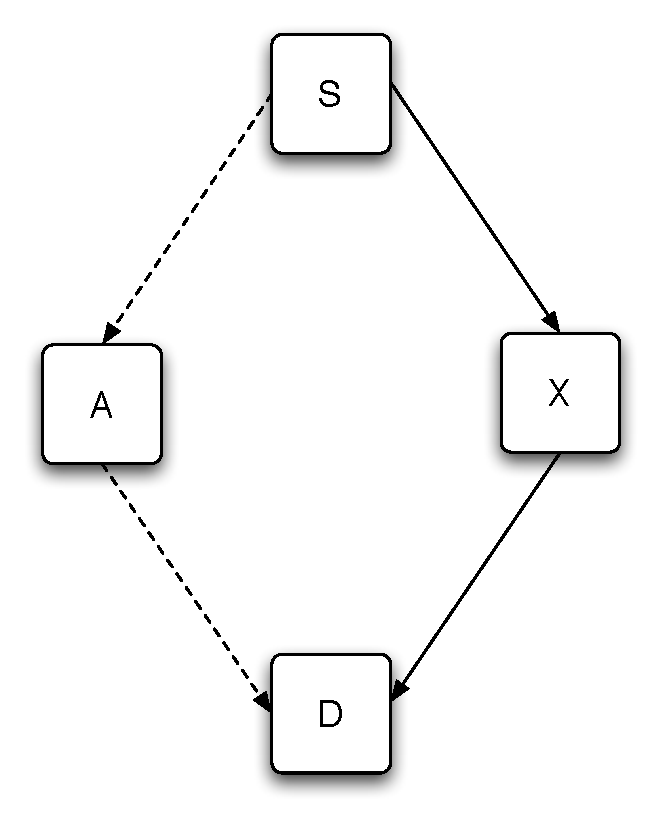
\includegraphics[width=0.3\textwidth]{SPFEEa}}
  \subfloat{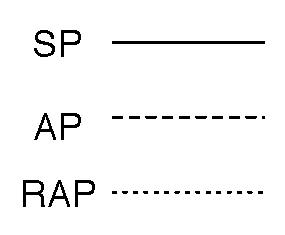
\includegraphics[width=0.2\textwidth]{SPFEELegend}}                 
  \setcounter{subfigure}{1}
  \subfloat[]{\label{fig:SPFEEb}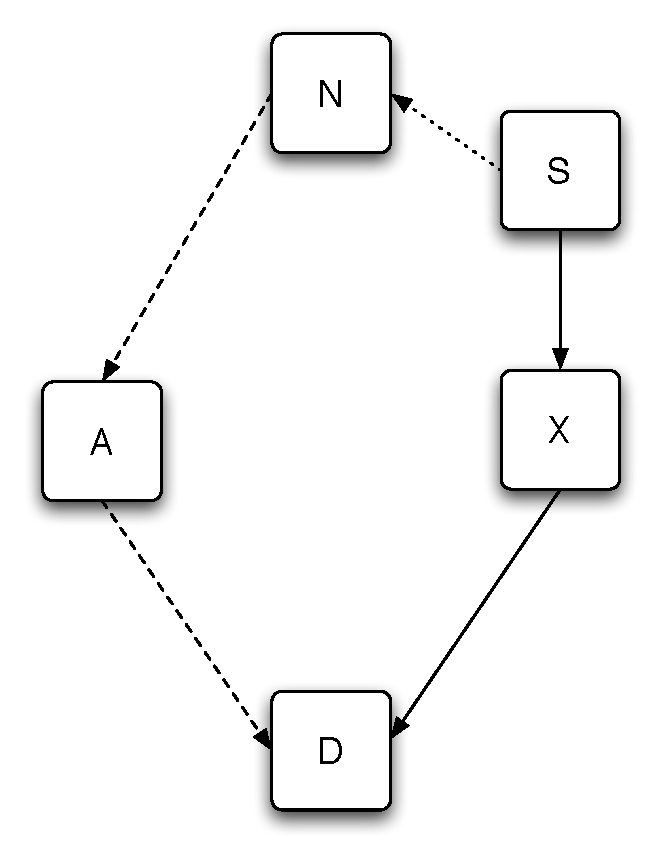
\includegraphics[width=0.3\textwidth]{SPFEEb}}
  \caption{An example of SPF-EE}
  \label{fig:SPFEE}
\end{figure}

%\ifigure{SPFEE}{0.5}{An example of SPF-EE.}{fig:SPFEE}

In the first case, the packet will simply travel from S to the alternative path (denoted by AP in Figure \ref{fig:SPFEE}) next hop (A) and then follow the shortest path from A to the destination as shown in Figure \ref{fig:SPFEEa}. The second case is more complicated as there are no downstream possibilities (assuming that all routing table updates have taken place, and therefore S knows that its shortest path is down) shown in Figure \ref{fig:SPFEEb}. Router S therefore sends a control packet to all its neighbors asking if they have an alternative path to the destination. If a neighbor router N finds a path then it sends the control packet back to S who then establishes a reverse alternative path (RAP), otherwise the neighbor propagates the request to its neighbor routers excluding S. 

The use of a control packet in SPF-EE is problematic because it increases the packet delay significantly while an alternative is found. Moreover, if the source router has no other neighbors other than the shortest path, the algorithm simply fails. A better solution would be to precompute the alternative path set in order to minimize the delay in the event of a failure.

SPF-EE only re-routes traffic in the event of an overload or a failure, another approach would be to take advantage of the path redundancy continuously. Adaptive MultiPath (AMP) \cite{AMP} does precisely that. AMP is based on providing routers with local network status information by exchanging so-called \textit{backpressure messages} (BM). Thus, enabling routers to adapt continuously to the changing network loads.

When AMP detects congestion on a link, it attempts to shift traffic away from this link. In order to achieve this, a router R connected to the congested link sends to its neighboring routers a BM indicating their contribution to the congested link. The neighboring router which receives this BM then notifies its neighbors of their contribution and so on. The routers then attempt to forward the congestion-inducing traffic onto other routes. Figure \ref{fig:AMP} illustrates the dispersion of the BMs when congestion originates from the Y routers.

\ifigure{AMP}{0.5}{An example of AMP.}{fig:AMP}

The issue with such an approach is that while router R knows how much traffic is sent to the individual Y routers, it generates a single value which is then sent back to router X in the form of a BM. Thereby the information which router X is interested in, namely its contribution to the congestion on a given path, is lost. By analyzing the structure of the BMs, we notice that every router needs to maintain a counter for each flow and store a reference of the flows origin because each router needs to compute a BM containing a value which is composed of the contributions of each individual flow, this clearly poses a scalability problem. The derivation of the BMs can be found in Section \ref{sect:AMPCALC}. 

\subsection{Multipath Routing Algorithms}

In 1998, Zauman introduced a new algorithm for the computation of multiple loop free paths from a source to a destination called Diffusing Algorithm for Shortest Multipath (DASM) \cite{DASM}. DASM is based on a generalization of the Diffusing Computations introduced by Dijkstra \cite{DijkstraTerm} and therefore it is also a generalization of DUAL \cite{DUAL} described in Section \ref{sect:DUAL}. DUAL only maintains a single next hop for any destination whereas DASM maintains a set of possible next hops. DASM introduces the concept of the \textit{Shortest Multipath}, which is an extension of DUAL's loop free routing along shortest paths. In DASM, the Shortest Multipath is guaranteed to be acyclic at the end of the diffusing computation.

%\newtheorem{def:shotestmulti}{Definiton}
\begin{definition}
  A \emph{shortest multipath} is defined by the directed acyclic graph obtained by the entries of the routing tables at each router in all paths from a source to a destination.
\end{definition}

\ifigure{DASM}{0.5}{An example of Shortest Multipath constructed with DASM.}{fig:DASM}

In order to ensure loop freeness, DASM constructs the Shortest Multipath graph by forcing routers to select next hops whose distance to the destination is less than their own. Figure \ref{fig:DASM}, illustrates the concept of Shortest Multipaths which contains the shortest path along with longer paths. It should be noted that each router computes the possible paths to the destination, therefore the shortest and longer paths at each router represent the shortest path and longer as computed from the current router.

A subsequent extension of DASM is presented in 2001 by Vutukury which provides loop freeness at every instant. Multipath Distance Vector Algorithm (MDVA) \cite{MDVA} is based on EDVA \cite{EDVA} algorithm presented in Section \ref{sect:DUAL}. To provide loop freeness at every instant MDVA makes sure that at every instant during a diffusing computation, a node who reports a distance via a next-hop K must keep K as its next hop at least until the end of the computation. Simply put, by using the loop free conditions enunciated by EDVA and the method to build multiple paths in DASM coupled with the invariance of reported distances during a computation, MDVA is capable of computing loop free multipaths at every instant.

 In link state algorithms, Vutukury proposed MPDA \cite{MPDA} which provides multiple paths of unequal costs to every destination which are loop free at every instant. The idea is to first compute multiple loop free paths using the same method as Near-OPT \cite{NearOPT}, but then use heuristics built on Gallager's Theorem \cite{Gallager-mindelay} to allocate flows to the computed paths and thereby approximating the optimal result presented in Near-OPT. MPDA sends updates to its neighbors and awaits their acknowledgement before sending another update, contrasting with previous algorithms who used diffusing computations which span the entire network, MPDA only sends out information to its neighbors and therefore its synchronization only spans a single hop.

%(see Section \ref{sect:GallagerAlgo})

Along the same lines as MPDA, Vutukury proposed MPATH \cite{MPATH1, MPATH2} which is a distance vector algorithm providing multiple loop free paths using only neighbor information. MPATH exchanges distances to destinations along with the predecessor to the destination, thereby allowing it to compute multipaths using only predecessor information. Similarly to MPDA, MPATH synchronizes only with its neighbors and therefore performs single hop synchronization. MPDA and MPATH differ only in the type of information their participating nodes exchange.

%see survey for help.

\section{Multipath Routing in current IP networks}


\subsection{OSPF Extensions}

\subsubsection{Equal Cost Multipath}
\label{sect:eqcostmulti}

OSPF defines a multipath protocol, called Equal Cost Multipath (ECMP) \cite{OSPF}, which only considers alternative paths of equal length to the shortest path, ie. each router maintains the set of possible next hops whose subsequent paths are of equal cost to the shortest solution. ECMP suffers from out of order packet arrival if routing decisions are taken packet per packet. To solve this problem several solutions are proposed by \cite{RFC2991}, which each define flows and then each flow is assigned to an outgoing port.

\begin{enumerate}
 \item \textbf{Modulo-N Hash} - The router performs a modulo-N operation over the hash of the packet headers which identity a flow. This method results in $\frac{N-1}{N}$ flow disruptions upon a link failure.
 \item \textbf{Hash-Threshold} - The router computes a hash of the packet headers used to identify a flow. The output range of the hash function is mapped against the number of possible next hops such that a the value of the computed hash will indicate which next hop to use. This method results in between $\frac{1}{4}$ and $\frac{1}{2}$ of all flows to be disrupted upon a link failure. This method is analyzed in \cite{RFC2992}. The analysis of the disruptions is given in Section \ref{sect:HTE}.
 \item \textbf{Highest Random Weight} - The router computes a key for each next-hop by computing a hash over the fields of a flow, as well the over the address for the next-hop \cite{HRW}. The key which obtains the highest value is selected and therefore so is the next-hop. This method involves N times the number of computation as in Modulo-N hash, but only $\frac{1}{N}$ flows are disrupted upon a link failure.
\end{enumerate}
%Above demonstrations to be given in the appendix?


An alternative approach is proposed by Vutukury \cite{TraffEngMinDelay} in which a key is appended by the source router to each packet belonging to a flow. This key is then used to by each router along the path to the destination to determine the next hop.

\subsubsection{OSPF Weights}

Fortz and Thorup \cite{TrafficEngOSPFWeights} and similarly Wang \cite{WANG01} propose methods to optimize the weights assigned to OSPF links. This centralized approach requires that the weights be precomputed assuming that the required load is known beforehand and that the network is quasi-static. Such assumptions make this solution unrealistic for an arbitrary network.

A typical and naive approach is to include a load metric with the standard distance metric \cite{Huitema}. The combination of these two metrics is then used to compute the shortest paths. This process therefore creates a feedback loop:

\begin{enumerate}
 \item A router receives an update for the different link loads and computes the new shortest paths.
 \item The traffic is now re-routed according to the new shortest paths. This causes the link loads to change and therefore,
 \item A new update message is generated and distributed.
\end{enumerate}

Feedback loops cause routes to oscillate and therefore create out of order packets, which as we have seen cause a significant performance loss. The frequency of the oscillations depends on the duration of the feedback loop. If the loop is slow, the number of oscillations is small but very little is gained over standard OSPF. On the other hand, if the loop is fast and many oscillations occur, we can expect many out of order packets and therefore very poor network performance.

\subsubsection{Optimized Multipath OSPF}

We have seen in the previous subsections techniques which attempt to divide traffic more or less equally among the available path sets. In 1998, Villamizar proposed OSPF Optimized Multipath (OMP) \cite{OMP} which takes into account path loads to distribute traffic efficiently among paths. OMP uses mechanisms already available in OSPF to flood the link information within a subnet \cite{RFC2370}.

Initially the algorithm computes the initial set of possible paths. Then the load on each link is iteratively adjusted according to the load information received from other routers. The following steps describe the process of building the path sets:

\begin{enumerate}
 \item Using a standard shortest path first algorithm the shortest paths to all destinations are computed.
 \item Construct a set of possible alternative paths by inspecting paths from neighbors to destinations and combining them with the links from a given router and these neighbors.
 \item Paths which then have equal costs or are within an acceptable margin of the minimum cost are kept. In order to avoid loops, paths which are longer than the minimal cost will only be kept if their immediate neighbor closer to the destination than the origin router.
\end{enumerate}

Once the possible path sets are established, the router can share load onto the paths. Routers will monitor the links and flood load information when the load changes. Depending on the overall network load, the flooding interval can be as large as 20 minutes if the load is low and 30 seconds otherwise. Every time a router receives new load information it will reexamine its load sharing as explained below:

\begin{enumerate}
 \item Examine all links and determine the critical links, and therefore establish the links with the highest load.
 \item Reduce the load on paths containing critical links.
 \item Increase the load on paths which do not contain critical links.
\end{enumerate}

OMP is still considered an experiment and has not yet been deployed in a production environment. However, it is very promising. In the next section we will discuss other load sharing algorithms which are research experiments.

\subsection{Alternative Methods}

In \cite{BAHK}, the authors introduce a routing scheme which is similar to the idea presented by SPF-EE \cite{SPFEE}. Under light traffic conditions, traffic is routed along the shortest path but as the load increases and congestion becomes significant the algorithm attempts to shift traffic onto less congested paths. To achieve this the algorithm uses two main concepts. The first is the classification of link states to identify more easily congested links. The second, is the computation of acceptable alternative paths which are within an acceptable margin of the shortest path in terms of hop count.

Load sensitive routing has always been hampered by the signaling overheads. Moreover, oscillations occur frequently in the path selection because the routing decisions are taken on out dated information. In \cite{LLIP}, the authors suggest a hybrid approach to solve the efficiency and stability issues, which relies on identifying long lived traffic flows and routing them separately. The algorithm provides load sensitive routing for long lived flows while forwarding short lived flows on preprovisioned static paths. In order to identify long lived flows and ensure stability, routers relate the detection of long lived flows to the timescale of signaling messages. 

A similar approach is suggested in \cite{LEE}, where packets are also grouped into flows to avoid out of order arrivals and long lived flows are also differentiated. Although in \cite{LEE}, the authors suggest that a minimum of flow states should be maintained by the router. This results that a flow is either routed on the primary (shortest) path or on the secondary (alternate) path depending on whether it is long lived or not. Figure \ref{fig:longvsshort} shows this load control mechanism: the flow classifier, identifies long lived flows and stores them in the flow table. Then the packet forwarding module forwards the packets according to the contents of the flow table.

\ifigure{flowclassifier}{0.5}{The flow classifier.}{fig:longvsshort}

A dynamic multipath routing (DPMR) scheme to improve resource utilization of a network carrying
real time traffic by re-routing on going flows through shorter routes is proposed in \cite{DMPR, DEDAS}. These approaches alleviate instantaneous congestion by allowing rerouting of a flow through a longer route. In contrast, in this paper, rerouting of an ongoing flow is allowed only if the new route is more preferable (i.e., shorter) than the current one. DMPR scheme works based on the route length, and is independent of the network congestion. 

\section{Summary}

In this section, we have presented the current state of the art in terms of multipath protocols. We have seen that the current protocols do not use multipath in a dynamic sense. Some protocols only consider paths of equal length, but these paths may not always be available. Other protocols introduce mechanisms for quick failover in case a path breaks. Finally, some protocols are simply not implementable as they will require too many resources. In the next sections, we will introduce models for multipath protocols and describe our congestion-aware protocols.
%Figure evolution from 28 to 32 

%summarize articles 28-32 see survey for help.
  


%\section{MPLS Networks}
%chap 5.

% ------------------------------------------------------------------------

%%% Local Variables: 
%%% mode: latex
%%% TeX-master: "../thesis"
%%% End: 

\chapter{Multipath Theory and Models}
\label{chap:theory}

\begin{flushright}
 \textit{\textquotedblleft In theory, theory and practice are the same. \\ 
In practice, they are not. \textquotedblright}\\
\textit{--Albert Einstein}
\end{flushright}

\ifpdf
    \graphicspath{{4-Theory/Chapter3Figs/PNG/}{4-Theory/Chapter3Figs/PDF/}{4-Theory/Chapter3Figs/}}
\else
    \graphicspath{{4-Theory/Chapter3Figs/EPS/}{4-Theory/Chapter3Figs/}}
\fi

In this chapter we will start by detailing the various graph algorithms used to compute shortest paths both in the Link State and Distance Vector scenarios. Next, we will describe the concept of Selfish routing which will provide a formal definition of the consequences of congestion insensitive routing. Finally, we will give a brief introduction and present the most remarkable results of Queue Theory which will be used later in this document to model our Multipath routing protocol.

%Then, we will give a description of the flow problems posed by Multipath routing which will provide insight why these algorithms are difficult if not impossible to implement in real networks.

\section{Graph Algorithms}
\label{sect:GraphAlgo}

The algorithms presented in this section do not provide multipath routes but only shortest paths. That said, they can be used, with some minor modifications, to build multipath routes as we will see in Chapter \ref{sect:multiroutes}.

\subsection{Dijkstra's Algorithm}

Dijkstra's Algorithm was proposed by Edsger Dijkstra in 1959 \cite{DIJK}, it is a graph search algorithm which given a graph composed of a set of edges, nodes and edge weights, finds the shortest path from a given source to all other nodes. It is therefore obvious that this algorithm is fundamental in Internet routing.

 The idea behind this algorithm is simple, consider a city's road system with intersections. You wish to find the shortest path between two points in this city. At your start point, you build a list of intersections which are directly connected to it. Then, select the intersection that is closest to your destination and mark the road and the starting intersection used. Next, repeat these steps considering the current intersection as your start point, considering one intersection at each iteration. Once the list of intersections is empty, the algorithm ends, and your shortest path is the the one consisting of all the marked intersections.

We will now give the algorithm description in textual form, the pseudo-code can be found in Section \ref{sect:dijkpseudo}, followed by a running example of the algorithm in Figure \ref{fig:runDijk}, the notation $\frac{x}{y|z}$ is used where x is the node name and y is the distance to the initial node and z the previous node. 

\begin{enumerate}
 \item Set the distance of the initial node to zero and infinity for all the others.
 \item Set all nodes to unvisited except the initial node (current node).
 \item For unvisited neighbors of the current node, compute their distance from the initial node. If this distance is less than their current distance, replace their current distance with the computed one.
 \item Once the distance for all unvisited neighbors have been computed, mark the current node as visited. 
 \item If no unvisited nodes remain, then the algorithm is finished. Otherwise pick the node with the smallest distance from the initial node and set it as the current node and repeat from step 3.
\end{enumerate}

\begin{figure}[!htbp]
\centering

\subfloat[Initial Graph.]{

\begin{tikzpicture}{shorten >=1pt, ->}
  \tikzstyle{every node} = [node distance = 2.5cm,
			    minimum size = 2mm,
			    inner sep = 2,
			    bend angle = 0]
\tikzset{EdgeStyle/.style={->}}
\SetVertexNoLabel
\Vertex{A0}

\NOEA(A0){A1}
\EA(A1){A2}
\SOEA(A0){A3}
\EA(A3){A4}
\AssignVertexLabel{A}{4}{$\frac{A}{0|-}$,$\frac{B}{\infty|-}$,$\frac{C}{\infty|-}$,$\frac{D}{\infty|-}$,$\frac{E}{\infty|-}$}
\tikzstyle{LabelStyle} = [above=6pt]
\Edge[label=$10$](A0)(A1)
\tikzstyle{LabelStyle} = [above=3pt]
\Edge[label=$5$](A0)(A3)
\Edge[label=$1$](A1)(A2)
\Edge[label=$2$](A3)(A4)
\Edge[label=$7$](A4)(A0)
\tikzstyle{LabelStyle} = [above=6pt]
\Edge[label=$9$](A3)(A2)
\tikzset{EdgeStyle/.append style = {bend left = 10}}
\tikzstyle{LabelStyle} = [right=3pt]
\Edge[label=$2$](A1)(A3)
\Edge[label=$4$](A2)(A4)
\tikzstyle{LabelStyle} = [left=3pt]
\Edge[label=$3$](A3)(A1)
\Edge[label=$6$](A4)(A2)

\end{tikzpicture}
}
\hspace{0.3cm}
\subfloat[Search for node closest to A.]{
\begin{tikzpicture}{shorten >=1pt, ->}
  \tikzstyle{every node} = [node distance = 2.5cm,
			    minimum size = 2mm,
			    inner sep = 2,
			    bend angle = 0]
\tikzset{EdgeStyle/.style={->}}
\SetVertexNoLabel
\Vertex{A0}

\NOEA(A0){A1}
\EA(A1){A2}
\SOEA(A0){A3}
\EA(A3){A4}
\AssignVertexLabel{A}{4}{$\frac{A}{0|-}$,$\frac{B}{10|A}$,$\frac{C}{\infty|-}$,$\frac{D}{5|A}$,$\frac{E}{\infty|-}$}
\tikzstyle{LabelStyle} = [above=6pt]
\tikzstyle{EdgeStyle} = [color = red, ->]
\Edge[label=$10$](A0)(A1)
\tikzstyle{LabelStyle} = [above=3pt]
\Edge[label=$5$](A0)(A3)
\tikzstyle{EdgeStyle} = [color = black, ->]
\Edge[label=$1$](A1)(A2)
\Edge[label=$2$](A3)(A4)
\Edge[label=$7$](A4)(A0)
\tikzstyle{LabelStyle} = [above=6pt]
\Edge[label=$9$](A3)(A2)
\tikzset{EdgeStyle/.append style = {bend left = 10}}
\tikzstyle{LabelStyle} = [right=3pt]
\Edge[label=$2$](A1)(A3)
\Edge[label=$4$](A2)(A4)
\tikzstyle{LabelStyle} = [left=3pt]
\Edge[label=$3$](A3)(A1)
\Edge[label=$6$](A4)(A2)

\end{tikzpicture}
}
\hspace{0.3cm}
\subfloat[D found, repeat search for closest node.]{
\begin{tikzpicture}{shorten >=1pt, ->}
  \tikzstyle{every node} = [node distance = 2.5cm,
			    minimum size = 2mm,
			    inner sep = 2,
			    bend angle = 0]
\tikzset{EdgeStyle/.style={->}}
\SetVertexNoLabel
\Vertex{A0}

\NOEA(A0){A1}
\EA(A1){A2}
\SOEA(A0){A3}
\EA(A3){A4}
\AssignVertexLabel{A}{4}{$\frac{A}{0|-}$,$\frac{B}{8|D}$,$\frac{C}{14|D}$,$\frac{D}{5|A}$,$\frac{E}{7|D}$}
\tikzstyle{LabelStyle} = [above=6pt]
\Edge[label=$10$](A0)(A1)
\tikzstyle{LabelStyle} = [above=3pt]
\tikzstyle{EdgeStyle} = [color = green, ->]
\Edge[label=$5$](A0)(A3)
\tikzstyle{EdgeStyle} = [color = black, ->]
\Edge[label=$1$](A1)(A2)
\tikzstyle{EdgeStyle} = [color = red, ->]
\Edge[label=$2$](A3)(A4)
\tikzstyle{EdgeStyle} = [color = black, ->]
\Edge[label=$7$](A4)(A0)
\tikzstyle{LabelStyle} = [above=6pt]
\tikzstyle{EdgeStyle} = [color = red, ->]
\Edge[label=$9$](A3)(A2)
\tikzset{EdgeStyle/.append style = {bend left = 10}}
\tikzstyle{LabelStyle} = [right=3pt]
\tikzstyle{EdgeStyle} = [color = black, ->,bend left = 10]
\Edge[label=$2$](A1)(A3)
\Edge[label=$4$](A2)(A4)
\tikzstyle{LabelStyle} = [left=3pt]
\tikzstyle{EdgeStyle} = [color = red, ->, bend left = 10]
\Edge[label=$3$](A3)(A1)
\tikzstyle{EdgeStyle} = [color = black, ->,bend left = 10]
\Edge[label=$6$](A4)(A2)

\end{tikzpicture}
}
\hspace{0.3cm}
\subfloat[Only consider node C, as others have already been found.]{
\begin{tikzpicture}{shorten >=1pt, ->}
  \tikzstyle{every node} = [node distance = 2.5cm,
			    minimum size = 2mm,
			    inner sep = 2,
			    bend angle = 0]
\tikzset{EdgeStyle/.style={->}}
\SetVertexNoLabel
\Vertex{A0}

\NOEA(A0){A1}
\EA(A1){A2}
\SOEA(A0){A3}
\EA(A3){A4}
\AssignVertexLabel{A}{4}{$\frac{A}{0|-}$,$\frac{B}{8|D}$,$\frac{C}{13|E}$,$\frac{D}{5|A}$,$\frac{E}{7|D}$}
\tikzstyle{LabelStyle} = [above=6pt]
\Edge[label=$10$](A0)(A1)
\tikzstyle{LabelStyle} = [above=3pt]
\tikzstyle{EdgeStyle} = [color = green, ->]
\Edge[label=$5$](A0)(A3)
\Edge[label=$2$](A3)(A4)
\tikzstyle{EdgeStyle} = [color = black, ->]
\Edge[label=$1$](A1)(A2)
\Edge[label=$7$](A4)(A0)
\tikzstyle{LabelStyle} = [above=6pt]
\Edge[label=$9$](A3)(A2)
\tikzset{EdgeStyle/.append style = {bend left = 10}}
\tikzstyle{LabelStyle} = [right=3pt]
\Edge[label=$2$](A1)(A3)
\Edge[label=$4$](A2)(A4)
\tikzstyle{LabelStyle} = [left=3pt]
\tikzstyle{EdgeStyle} = [color = red, ->, bend left = 10]
\Edge[label=$6$](A4)(A2)
\tikzstyle{EdgeStyle} = [color = green, ->, bend left = 10]
\Edge[label=$3$](A3)(A1)

\end{tikzpicture}
}
\hspace{0.3cm}
\subfloat[Consider only C again, for the same reason.]{
\begin{tikzpicture}{shorten >=1pt, ->}
  \tikzstyle{every node} = [node distance = 2.5cm,
			    minimum size = 2mm,
			    inner sep = 2,
			    bend angle = 0]
\tikzset{EdgeStyle/.style={->}}
\SetVertexNoLabel
\Vertex{A0}

\NOEA(A0){A1}
\EA(A1){A2}
\SOEA(A0){A3}
\EA(A3){A4}
\AssignVertexLabel{A}{4}{$\frac{A}{0|-}$,$\frac{B}{8|D}$,$\frac{C}{9|B}$,$\frac{D}{5|A}$,$\frac{E}{7|D}$}
\tikzstyle{LabelStyle} = [above=6pt]
\Edge[label=$10$](A0)(A1)
\tikzstyle{LabelStyle} = [above=3pt]
\tikzstyle{EdgeStyle} = [color = green, ->]
\Edge[label=$5$](A0)(A3)
\Edge[label=$2$](A3)(A4)
\tikzstyle{EdgeStyle} = [color = red, ->]
\Edge[label=$1$](A1)(A2)
\tikzstyle{EdgeStyle} = [color = black, ->]
\Edge[label=$7$](A4)(A0)
\tikzstyle{LabelStyle} = [above=6pt]
\Edge[label=$9$](A3)(A2)
\tikzset{EdgeStyle/.append style = {bend left = 10}}
\tikzstyle{LabelStyle} = [right=3pt]
\Edge[label=$2$](A1)(A3)
\Edge[label=$4$](A2)(A4)
\tikzstyle{LabelStyle} = [left=3pt]
\Edge[label=$6$](A4)(A2)
\tikzstyle{EdgeStyle} = [color = green, ->, bend left = 10]
\Edge[label=$3$](A3)(A1)

\end{tikzpicture}
}
\hspace{0.3cm}
\subfloat[Green edges show the final shortest path graph.]{
\begin{tikzpicture}{shorten >=1pt, ->}
  \tikzstyle{every node} = [node distance = 2.5cm,
			    minimum size = 2mm,
			    inner sep = 2,
			    bend angle = 0]
\tikzset{EdgeStyle/.style={->}}
\SetVertexNoLabel
\Vertex{A0}

\NOEA(A0){A1}
\EA(A1){A2}
\SOEA(A0){A3}
\EA(A3){A4}
\AssignVertexLabel{A}{4}{$\frac{A}{0|-}$,$\frac{B}{8|D}$,$\frac{C}{9|B}$,$\frac{D}{5|A}$,$\frac{E}{7|D}$}
\tikzstyle{LabelStyle} = [above=6pt]
\Edge[label=$10$](A0)(A1)
\tikzstyle{LabelStyle} = [above=3pt]
\tikzstyle{EdgeStyle} = [color = green, ->]
\Edge[label=$5$](A0)(A3)
\Edge[label=$2$](A3)(A4)
\Edge[label=$1$](A1)(A2)
\tikzstyle{EdgeStyle} = [color = black, ->]
\Edge[label=$7$](A4)(A0)
\tikzstyle{LabelStyle} = [above=6pt]
\Edge[label=$9$](A3)(A2)
\tikzset{EdgeStyle/.append style = {bend left = 10}}
\tikzstyle{LabelStyle} = [right=3pt]
\Edge[label=$2$](A1)(A3)
\Edge[label=$4$](A2)(A4)
\tikzstyle{LabelStyle} = [left=3pt]
\Edge[label=$6$](A4)(A2)
\tikzstyle{EdgeStyle} = [color = green, ->, bend left = 10]
\Edge[label=$3$](A3)(A1)

\end{tikzpicture}
}
\caption{Running Example of Dijkstra's Algorithm}
\label{fig:runDijk}
\end{figure}

As is shown by Figure \ref{fig:runDijk}, Dijkstra's Algorithm grows a tree from a given source to all the other nodes for which the distance from the source to all the other nodes is minimal. We initially start with the original graph at node A which has a cost of zero. In the second step, we start at A and search for its closest neighbor (red arrows), we than remove A from the list of unvisited nodes (Q). Next, having found D as the closest neighbor, we can safely mark the edge from A to D as part of the shortest path (green arrow). We then repeat the search for D and find E and remove D from Q. At E we only consider the edge to C as the others link to nodes which are no longer in Q. At the end, we obtain the green graph which is the shortest path from A to all the other nodes. Table \ref{tab:runDijk} shows the intermediate steps in the algorithm, the notation x/y is used where x represents the distance from the initial node and y is the precedent node in the shortest path.

\begin{table}[!htbp]
\begin{center}
\begin{tabular}[]{|c|c|c|c|c|c|c|c|}
$I$ & A   & B          & C          & D          & E         & Q  & Path Nodes \\
0   & 0/- & $\infty/-$ & $\infty/-$ & $\infty/-$ &$\infty/-$ & A-E & $\varnothing$ \\
1   & 0/- & 10/A 	     & $\infty/-$ & 5/A        &$\infty/-$ & B-E & A \\
2   & 	& 8/D 	     & 14/D 	  & 5/A        & 7/D 	   & B,C,E & A,D \\
3   & 	& 8/D 	     & 13/E 	  & 	       & 7/D 	   & B,C & A,D,E \\
4   & 	& 8/D 	     & 9/B 	  & 	       & 	   & C & A,D,E,B \\
5   & 	& 	     	     & 9/B 	  & 	       & 	   & $ \varnothing $ & A,D,E,B,C
\end{tabular}
\end{center}
\caption{Step by Step of Dijkstra's Algorithm}
\label{tab:runDijk}
\end{table}

\subsection{Bellman-Ford Algorithm}

 Bellman-Ford's algorithm \cite{Bellman1958} is the basis for Distance Vector routing protocols. It was proposed simultaneously by Bellman and Ford in 1958. It produces the same result as Dijkstra's algorithm but it is more flexible, namely it allows for negative edge weights\footnote{While this is an interesting fact, it is useless for internet routing. Indeed, negative weights have no physical meaning.}. It is a decentralized algorithm which only requires nodes to inform its neighbors of their distances to other nodes. Then, each node receiving this information picks the shortest advertised weight. 

In a network, routers which use this algorithm maintain a distance table containing an entry for each of the nodes in the network. By looking up in the distance table, a router will know where to send traffic intended for a particular destination. Below we give a textual description of the algorithm, whose pseudo-code can be found in Section \ref{sect:bellpseudo} followed by a running example of the algorithm.

\begin{itemize}
 \item Initialize the graph by setting all distances to $\infty$ and the source's distance to zero.
 \item If the distance from the source to a neighbor using a particular edge is shorter than the current distance, overwrite the current distance with the new one. Repeat this step for all nodes and reconsider all edges in the graph.
 \item Finally check for negative edge cycles by computing the distance from a node to its neighbor, if this distance is smaller than the stored distance then the graph contains negative edge weights.
\end{itemize}

The order in which the edges are visited is not specified by the algorithm, therefore we will opt to visit, from left to right, the top horizontal edges first, then the vertical ones, followed by the bottom horizontal ones, and leave the diagonal ones last. The notation is the same as in the case of Dijkstra. 

\begin{figure}[!htbp]
\centering

\subfloat[Initial Graph]{

\begin{tikzpicture}{shorten >=1pt, ->}
  \tikzstyle{every node} = [node distance = 2.5cm,
			    minimum size = 2mm,
			    inner sep = 2,
			    bend angle = 0]
\tikzset{EdgeStyle/.style={->}}
\SetVertexNoLabel
\Vertex{A0}

\NOEA(A0){A1}
\EA(A1){A2}
\SOEA(A0){A3}
\EA(A3){A4}
\AssignVertexLabel{A}{4}{$\frac{A}{0|-}$,$\frac{B}{\infty|-}$,$\frac{C}{\infty|-}$,$\frac{D}{\infty|-}$,$\frac{E}{\infty|-}$}
\tikzstyle{LabelStyle} = [above=6pt]
\Edge[label=$10$](A0)(A1)
\tikzstyle{LabelStyle} = [above=3pt]
\Edge[label=$5$](A0)(A3)
\Edge[label=$1$](A1)(A2)
\Edge[label=$2$](A3)(A4)
\Edge[label=$7$](A4)(A0)
\tikzstyle{LabelStyle} = [above=6pt]
\Edge[label=$9$](A3)(A2)
\tikzset{EdgeStyle/.append style = {bend left = 10}}
\tikzstyle{LabelStyle} = [right=3pt]
\Edge[label=$2$](A1)(A3)
\Edge[label=$4$](A2)(A4)
\tikzstyle{LabelStyle} = [left=3pt]
\Edge[label=$3$](A3)(A1)
\Edge[label=$6$](A4)(A2)

\end{tikzpicture}
}
\hspace{0.3cm}
\subfloat[At node B, update distances according to edge traversal order]{

\begin{tikzpicture}{shorten >=1pt, ->}
  \tikzstyle{every node} = [node distance = 2.5cm,
			    minimum size = 2mm,
			    inner sep = 2,
			    bend angle = 0]
\tikzset{EdgeStyle/.style={->}}
\SetVertexNoLabel
\Vertex{A0}

\NOEA(A0){A1}
\EA(A1){A2}
\SOEA(A0){A3}
\EA(A3){A4}
\AssignVertexLabel{A}{4}{$\frac{A}{0|-}$,$\frac{B}{8|D}$,$\frac{C}{11|B}$,$\frac{D}{5|A}$,$\frac{E}{7|D}$}
\tikzstyle{LabelStyle} = [above=6pt]
\Edge[label=$10$](A0)(A1)
\tikzstyle{LabelStyle} = [above=3pt]
\tikzstyle{EdgeStyle} = [color = green, ->]
\Edge[label=$5$](A0)(A3)
\Edge[label=$2$](A3)(A4)
\tikzstyle{EdgeStyle} = [color = black, ->]
\Edge[label=$1$](A1)(A2)
\Edge[label=$7$](A4)(A0)
\tikzstyle{LabelStyle} = [above=6pt]
\Edge[label=$9$](A3)(A2)
%\tikzset{EdgeStyle/.append style = {bend left = 10}}

\tikzstyle{EdgeStyle} = [color = green, ->, bend left = 10]
\tikzstyle{LabelStyle} = [left=3pt]
\Edge[label=$3$](A3)(A1)
\tikzstyle{LabelStyle} = [right=3pt]
\tikzstyle{EdgeStyle} = [color = black, ->, bend left = 10]
\Edge[label=$4$](A2)(A4)
\Edge[label=$2$](A1)(A3)
\tikzstyle{LabelStyle} = [left=3pt]
\Edge[label=$6$](A4)(A2)

\end{tikzpicture}
}
\subfloat[Update distance for node C, since it was missed in the last iteration.]{

\begin{tikzpicture}{shorten >=1pt, ->}
  \tikzstyle{every node} = [node distance = 2.5cm,
			    minimum size = 2mm,
			    inner sep = 2,
			    bend angle = 0]
\tikzset{EdgeStyle/.style={->}}
\SetVertexNoLabel
\Vertex{A0}

\NOEA(A0){A1}
\EA(A1){A2}
\SOEA(A0){A3}
\EA(A3){A4}
\AssignVertexLabel{A}{4}{$\frac{A}{0|-}$,$\frac{B}{8|D}$,$\frac{C}{9|B}$,$\frac{D}{5|A}$,$\frac{E}{7|D}$}
\tikzstyle{LabelStyle} = [above=6pt]
\Edge[label=$10$](A0)(A1)
\tikzstyle{LabelStyle} = [above=3pt]
\tikzstyle{LabelStyle} = [above=6pt]
\Edge[label=$10$](A0)(A1)
\tikzstyle{LabelStyle} = [above=3pt]
\tikzstyle{EdgeStyle} = [color = green, ->]
\Edge[label=$5$](A0)(A3)
\Edge[label=$2$](A3)(A4)
\Edge[label=$1$](A1)(A2)
 \tikzstyle{EdgeStyle} = [color = black, ->]
\Edge[label=$7$](A4)(A0)
\tikzstyle{LabelStyle} = [above=6pt]
\Edge[label=$9$](A3)(A2)
%\tikzset{EdgeStyle/.append style = {bend left = 10}}
\tikzstyle{EdgeStyle} = [color = green, ->, bend left = 10]
\tikzstyle{LabelStyle} = [left=3pt]
\Edge[label=$3$](A3)(A1)
\tikzstyle{LabelStyle} = [right=3pt]
\tikzstyle{EdgeStyle} = [color = black, ->, bend left = 10]
\Edge[label=$4$](A2)(A4)
\Edge[label=$2$](A1)(A3)
\tikzstyle{LabelStyle} = [left=3pt]
\Edge[label=$6$](A4)(A2)
\end{tikzpicture}
}

\caption{Running Example of Bellman-Ford's Algorithm}
\label{fig:runBell}
\end{figure}

It may seem in Figure \ref{fig:runBell}, that Bellman-Ford's algorithm is extremely efficient. This is not the case, because for each node it analyses every edge in the network, this is not shown for reasons of brevity and clarity. Bellman-Ford therefore requires  O($|V| |E|$) operations, whereas Dijkstra's algorithm requires O($|E|+ |V|log|V|$), where $|V|$ is the number of vertices's and $|E|$ the number of edges.

%\section{Flow Problems}
%\label{sect:flow}
%nonlinear multicommodity flow problem

%\subsection{Gallager's Algorithm}
%\label{sect:GallagerAlgo}

\section{Selfish Routing}

Selfish routing describes the overall negative effects on the performance of a network when routing decisions are taken selfishly. It is clear that the travel time between two points is highly dependant on the number of users using a given route. Yet, most of us will always opt for the shortest path that gets us to our destination fastest, regardless of the effect this decision has on other users. This is referred to as Selfish Routing \cite{Selfish}.

Routing on the Internet is insensitive to congestion and therefore suffers from the phenomena explained by Selfish routing. Indeed, shortest path routing is analogous to commuters traveling to work each choosing the shortest path and thereby delaying everyone. Figure \ref{fig:pigou} shows a network (referred to as Pigou's Example \cite{Pigou}), in which the total traffic is represented by one, with two paths where the upper one has a delay of one time unit regardless of congestion and the lower path's delay is a function of the congestion. It is reasonable to assume that all traffic will be selfishly routed along the lower path, and therefore that it will be delayed by one time unit. On the other hand, if we consider that the traffic is split equally between the two paths, the overall delay is $\frac{3}{4}$. Indeed, the traffic on the upper path suffers a delay of one time unit but now the traffic on the lower path is only delayed by half a time unit. Therefore, we easily see that no traffic is worse off and moreover half of the traffic is delivered significantly faster. Clearly, the phenomenon illustrated in the first situation could be offset by increasing the link capacities but this is not a tenable nor scalable solution in the longterm.

\begin{figure}[h!]
\begin{center}
\begin{tikzpicture}[>=latex']
 \SetUpEdge[lw         = 2.0pt,
           color      = black],
          labelcolor = black!30],
          labelstyle = {draw,thick,-}]
  %\tikzstyle{edge} = [draw,thick,-]
  \tikzset{node distance = 5.0cm}
  \GraphInit[vstyle=Normal]
  \tikzset{EdgeStyle/.style={->}}
  \tikzset{EdgeStyle/.append style = {bend left = 30}}
  \Vertex{S}
  \EA(S){D}

  \Edge[label=$d(x) {=} 1$](S)(D)
  \tikzset{EdgeStyle/.style={<-}}
  \tikzset{EdgeStyle/.append style = {bend left = 30}}
  \Edge[label=$d(x) {=} x$](D)(S)

\end{tikzpicture}
\end{center}
\caption{Pigou's Example}
\label{fig:pigou}
\end{figure}

%- define a nash flow
%- define optimal flow
%  - price of anarchy worst possible ratio between a selfish routing instance and an optimal instance.
%- define the price of anarchy

Selfish Routing also provides us with a further justification of deploying multipath routing protocols. Before we develop further this justification we must first proceed to the definitions of a few concepts which are more formally detailed in Section \ref{sect:linearanarchy}. First, we must redefine the notion of a flow which will be limited to this section only.

\begin{definition}
  A \emph{flow} $f$ is interpreted as the aggregated routes chosen by the traffic, with $f_p$ measuring the amount of traffic on route $p$.
\end{definition}

\textbf{Note:} The term flow used here differs significantly from our previous definition. This definition only hold for this section and during the rest of this document we will revert to our previous definition.

\begin{itemize}
 \item \emph{Nash Flow} can be seen as a flow routed selfishly, as in the first case given in Figure \ref{fig:pigou}.
 \item \emph{Optimal Flow} is the flow with minimum possible delay, as in the second case of Figure \ref{fig:pigou}.
 \item \emph{Price of Anarchy} is the \emph{worst-possible} ratio between the delay of a Nash flow and that of an optimal flow.
\end{itemize}

With these definitions at hand and if we consider multipath networks with only linear delay functions, Selfish routing tells us that the upper bound\footnote{An upper bound also exists for all polynomial delay functions, which is given in Section \ref{sect:linearanarchy}, but for the sake of clarity we only refer to linear cost functions here.} on the \emph{Price of Anarchy} is $\frac{4}{3}$ (see proof in Section \ref{sect:linearanarchy}). This result further justifies our exploration of multipath networks, because in a multipath network with selfish users it would be expected that additional problems in congestion would arise and therefore deteriorate the performance of the network. This result shows us that this is not the case, and that even in a multipath network with only selfish users there is ``only'' about a 33\% loss in performance, which gives us hope that we may improve the performance of a multipath network significantly while paying a relatively small price in the worst-case scenario (ie. only shortest paths available). Indeed, as we will see in the next chapter, our protocol attempts to leverage all feasible alternative paths and defaults to the shortest path (selfish route) if the alternative paths are not available. As the delay functions increase in degree (ie. polynomial delay functions), the Price of Anarchy increases as well.

%- show that the upper bound for multipath networks is 4/3 --> a 1/3 loss in performance.
%- This shows us that in a multicommodity network, extra obstruction caused by selfish agents do not arise and therefore provides us with an extra justification to proceed in our exploration of a multipath protocol while suggesting that there is yet room for improvement.


\section{Analytical Models}

In this section we present some analytical models based on Queuing Theory which will allow us to model multipath protocols. It should be stated that an exact analysis of multipath communication is too complex \cite{CommNets}, however the independence assumption of Section \ref{sect:kleindep} simplifies the calculations and provides a reasonable approximation. 

\subsection{Queue Theory}
\label{sect:queues}

A queuing system \cite{KLEVol1}, as shown in Figure \ref{fig:queue} is characterized by the following parameters:

\ifigure{queue}{0.5}{A standard queue.}{fig:queue}

\begin{itemize}
 \item \textit{Arrival process (A)} is defined by the distribution of the inter-arrival time of clients into the queue. The only interesting arrival process in this thesis is exponential (Markovian).
 \item \textit{Service time distribution (B)} represents the time required to serve a client present at the top of the queue. We will only deal with Markovian distributions.
 \item \textit{Number of servers (m)} present in a single queue. We will deal with models containing one or more servers.
 \item \textit{Capacity (K)} of the queue is the maximum number of clients which can be present in the system at any given moment.
 \item \textit{Population size (N)} represents the potential number of clients whether finite or infinite. We will consider situations with infinite populations.
 \item \textit{Queuing policy (D)} defines in which order the next client is selected from the queue, eg. first in, first out (FIFO).
\end{itemize}

\textit{Kendall's Notation} is often used to identify the type of queue used which is denoted by A/B/m/K/N/D. The parameters K, N, and D are often omitted indicating that they are either infinite or that a FIFO policy is used. 

The arrival and service time processes can be either of the following:

\begin{itemize}
 \item \textit{Markovian} - A Poisson distribution \cite{Poisson} where the inter-arrival times are independent and exponentially distributed.
 \item \textit{Deterministic} - constant inter-arrival/service time.
 \item \textit{General Distribution} where the underlying probability density function is arbitrary.
\end{itemize}

It is worth presenting some general results and notations which apply to all queuing systems:

\begin{itemize}
 \item $\lambda$ is the average inter arrival rate of clients into the systems.
 \item $\frac{1}{\mu}$, the average service time per server.
 \item $\rho$ is the utilization factor of the queue ($\frac{\lambda}{\mu}$ and $\frac{\lambda}{m\mu}$ in the multi-server case). For the queue to be stable, we should have $0 \leq \rho < 1$.
\item $T$ is the total average time in the system (queue + service).
\begin{equation}
 T = W + \frac{1}{\mu} = \frac{1}{\mu - \lambda}
 \label{eq:GG1T}
\end{equation}
 \item $W$ is the average waiting time in the queue.
 \begin{equation}
 W = \frac{\rho}{\mu - \lambda}
 \label{eq:GG1W}
\end{equation}
 \item $\bar{N}$ is the average number of clients in the system given by Little's Result \cite{little}.
\begin{equation}
  \bar{N} = \lambda T
 \label{eq:Little}
\end{equation}
 \item $\bar{N}_q$ is the average size of the queue.
\begin{equation}
 \bar{N}_Q = \bar{N} - m\rho
 \label{eq:GG1NQ}
\end{equation}

 
 \item $P_N$ is the probability that there are N clients in the system.
\end{itemize}

In the next sections we will present remarkable results for both the M/M/1 and M/M/m queues. We will also describe Kleinrock's Independence Assumption. 

\subsubsection{M/M/1 Queue}

The M/M/1 queue is composed of exponentially distributed inter-arrival process and service times along with a single server model. The M/M/1 queue is the simplest form a queue can take, while still remaining interesting. While being simple its behavior is similar to other more complex cases. 

Since the inter arrival distribution is Poisson, the arrival rate is given by $\lambda$ and the service time is $\frac{1}{\mu}$, which gives us directly the following relations:

\begin{equation}
\bar{N} = \frac{\rho}{1-\rho}
\label{eq:MM1N}
\end{equation}
 
Using Little's Result (Equation \ref{eq:Little}) and Equation \ref{eq:GG1NQ}, we obtain the following relations for $W$ and $T$.

\begin{equation}
W = \frac{\rho}{\mu(1-\rho)} 
\label{eq:MM1W}
\end{equation}

and,

\begin{equation}
T = \frac{1}{\mu(1-\rho)}
\label{eq:MM1T}
\end{equation}

\begin{figure}[htbp!]
\begin{center}

\begin{tikzpicture}[scale=1.0, domain=0:9.8]
    \draw[very thin,color=gray,step=.5cm] (-0.1,-0.1) grid (10.2,10.2);
    \draw[->] (-0.2,0) -- (10.2,0) node[below = 28pt, left=50pt] {$\rho \rightarrow$};
    \draw[->] (0,-0.2) -- (0,10.2) node[left = 28pt, below=5pt] {$\rotatebox{90}{T}$};
    \draw[dotted](10,0) -- (10,10);
    \foreach \x/\xtext in {10/1}
      \draw[shift={(\x,0)}] (0pt,2pt) -- (0pt,-2pt) node[below] {$\xtext$};
    \foreach \y/\ytext in {2/\frac{1}{\mu}}
    \draw[shift={(0,\y)}] (2pt,0pt) -- (-2pt,0pt) node[left] {$\ytext$};

%MODIFIED BY HAND

    \draw[color=black] plot[id=delay] function{(1/(1-(x/10)))};


\end{tikzpicture}
\end{center}
\caption{Average delay as a function of $\rho$.}
\label{fig:MM1INF}
\end{figure}

%\ifigure{MM1INF}{0.8}{Average delay as a function of $\rho$.}{fig:MM1INF}

All the relations given for $\bar{N}$, $T$, and $W$ demonstrate common behavior with respect to the utilization factor $\rho$, more precisely they behave inversely to $1 - \rho$. Therefore, as $\rho$ tends towards one the average delays and queue sizes tend towards infinity as shown in Figure \ref{fig:MM1INF}.


\subsubsection{M/M/m Queue}
\label{sect:mmmQ}

We will now consider a generalization of the M/M/1 queue to m servers. In this model, a single queue forms the entry to the system and a collection of servers will handle the first client at the head of the queue. As previously, $\lambda$ is the arrival rate and $\frac{1}{\mu}$ is the average service time. Also, we have here that $\rho = \frac{\lambda}{m\mu}$.

Before presenting the steady state relations relative to an M/M/m queue, we must first distinguish the situations where the queue is busy and when it is not, which help establish the steady state relations. This is given by the probability of finding that all servers are busy when a new client arrives:

\begin{equation}
P_{Q} = \frac{p_{0}(m\rho)^{m}}{m!(1-\rho)}
\label{eq:MMMPQ}
\end{equation}

where,

\begin{equation}
p_{0} = \left[ \displaystyle\sum\limits_{n=0}^{m-1} \frac{(m\rho)^{n}}{n!} + \frac{(m\rho)^{m}}{m!(1-\rho)}\right]^{-1}
\label{MMMP0}
\end{equation}

$P_{Q}$ is known as the \emph{Erlang C formula} \cite{Erlang} and is widely used in telephony. Now we give the following relations for the number of clients in the system and in the queue, respectively. The complete derivation of these relations can be found in cite{KLEVol1} and other Queuing Systems literature, the author only wishes to remind them here.

\begin{equation}
 \bar{N} = m\rho + \frac{\rho P_{Q}}{1-\rho}
\label{eq:MMMN} 
\end{equation}

and,

\begin{equation}
\bar{N}_Q = \frac{\rho P_{Q}}{1 - \rho}
\label{eq:MMMNQ} 
\end{equation}


Using Little's Result (Equation \ref{eq:Little}) and Equation \ref{eq:GG1NQ}, we obtain the following relations for the average time (network delay) and the average waiting time (forwarding and processing time) spent in the system, respectively.

\begin{equation}
 T = \frac{1}{\mu}\left(1 + \frac{P_{Q}}{m(1-\rho)}\right)
\label{eq:MMMT} 
\end{equation}

and,

\begin{equation}
 W = \frac{P_{Q}}{m\mu\left(1-\rho\right)}
\label{eq:MMMW} 
\end{equation}
%\subsubsection{Jackson's Theory - Networks of Queues}

\subsubsection{Kleinrock's Independence Assumption}
\label{sect:kleindep}
% ------------------------------------------------------------------------
In the two models, presented above, we have assumed that both the arrival and service times respect the Markovian property, ie. the future state of the system depends only on the present state. Moreover Burke's Theorem \cite{Burke} states:

\newtheorem{theorem}{Theorem}
\begin{theorem}
\label{th:Burke}
\textbf{Burke's Theorem.} The steady-state output of a queue with N channels in parallel, with Poisson arrivals and message lengths chosen independently from an exponential distribution is itself Poisson-distributed. 
\end{theorem}

Consider now the situation, which exists within data networks, where many queues interact in the sense that the output from one queue is the input of another (or possibly several others). Given Burke's Theorem and the models we have presented, one might think that delays in data networks are simple to obtain via such models. Unfortunately this is not the case, the message (or packet) inter-arrival time and the message lengths beyond the first queue in the network become strongly dependent. Due to the fact that the service times at each queue are a function of the message length and therefore the arrival time at each subsequent queue is no longer Markovian \cite{CommNets}.

%\ifigure{tandem}{0.7}{A tandem network.}{fig:tandem}

\tikzstyle{vertex}=[circle,fill=black,minimum size=10pt,inner sep=0pt]
\tikzstyle{texver} = [circle, fill=black!25, minimum size = 20pt]
\tikzstyle{edge} = [draw,thick,->]

\begin{figure}[htbp!]
\begin{center}
\begin{tikzpicture}[scale=1.8, auto,swap]
 \foreach \pos/\name in {{(0,0)/0}, {(3,0)/3}}
        \node[vertex]   (\name) at \pos {};
        
  \foreach \pos/\name in {{(1,0)/1}, {(2,0)/2}}
        \node[texver] (\name) at \pos {$\name$};

\foreach \source/ \dest in {0/1,1/2,2/3}
        \path[edge] (\source) -- (\dest);
	

\end{tikzpicture}
\caption{A tandem network.}
\label{fig:tandem}
\end{center}
\end{figure}


Figure \ref{fig:tandem} illustrates two queues in tandem where packet lengths are exponentially distributed and independent of each other as well as the inter-arrival times at the first queue. We can therefore state that the first queue follows the M/M/1 model, but we cannot say the same about the second queue because the inter-arrival times at the second queue are strongly correlated with the packets lengths. Indeed the inter-arrival time at the second queue is \textbf{equal} to the transmission time at the first queue. As an analogy to this situation, consider a truck traveling on a narrow busy road along with several fast cars. Typically the truck will see an empty road ahead of it while it is being closely followed by a line of cars. The dependence between inter-arrival and message lengths (and therefore service time) is a source of great mathematical complexity for the analysis of queuing networks, in which even the simple case of the tandem network has no known exact solution \cite{DataNetworks}. A full mathematical demonstration of this dependence is given in Section \ref{sect:KLEDEP}.

As previously shown the dependence appears for queues which are internal to the network. Therefore, one might ask: Why is there a difference between the initial (network entry) queue and internal queues? The answer is straightforward, the initial queue receives its messages from an external source consisting of many subscribers (in our case people or computers) which are all generating messages. The overall message generation by the subscribers exhibits an independence \cite{CommNets} since one message is different from one person to the next. In a general network a similar situation exists. Indeed, more than one queue can deliver messages to any given queue, similarly any given queue is receiving messages from many other queues. If we accept this observation then we can define the following assumption:

%\newtheorem{}{Theorem}
\begin{theorem}
\label{th:indep}
\textbf{Independence Assumption.} Each time a message is received at a queue within the net, a new length $v$ is chosen for this message from the following distribution:

\begin{center}
 $P(v) = \mu e^{-\mu v}$
\end{center} 
\end{theorem}

Obviously, such an assumption does not correspond to the reality with a general network. Nevertheless, it results in a far simpler mathematical modeling of networks, while still maintaining an acceptable degree of accuracy \cite{CommNets}. 


\section{Summary}

This section has presented the modeling tools that we have used to describe our protocols. As we have shown, it is clearly beyond the scope of this document to attempt to describe multipath networks accurately due to the sheer mathematical complexity involved. 

We have also discussed and given justification for deploying multipath protocols. While the use of multipath may seem evident, using longer paths rather than only the shortest path is less clear. We have seen that routing selfishly (ie. always onto the shortest path), causes the performance to drop significantly.
%%% Local Variables: 
%%% mode: latex
%%% TeX-master: "../thesis"
%%% End: 

\chapter{The MultiRoute Family}
\label{chap:cornerstones}
\label{sect:multiroutes}
\begin{flushright}
 \textit{\textquotedblleft There is always a better strategy than the one you
have; \\ 
you just haven't thought of it yet\textquotedblright}\\
\textit{-- Sir Brian Pitman}
\end{flushright}


\ifpdf
    \graphicspath{{5-CornerMultipath/Chapter5Figs}{5-CornerMultipath/Chapter5Figs/PDF/}{5-CornerMultipath/Chapter5Figs/}}
\else
    \graphicspath{{5-CornerMultipath/Chapter5Figs/EPS/}{5-CornerMultipath/Chapter5Figs/}}
\fi

We now present the MultiRoute suite of congestion-aware inter-gateway routing protocols. But
first, we should define the path discovery strategy employed by MultiRoute
variants as it is identical and fundamental to all protocols. Then, we will
describe MultiRoute Monitoring Protocol (MMP) which is responsible for the
dissemination of congestion information throughout the network. While it differs
slightly from protocol to protocol, its essential basis stays unchanged within
each protocol. 

Next, we will follow RFC 1264 \cite{RFC1264} which describes the procedures for
creating and documenting standards on routing protocols. While this RFC has
been obsoleted for practical reason, the author still believes that some
aspects of the RFC can be used.


\section{Path Discovery}


Modern computer networks may offer many paths from any source to any
destination but current protocols only employ the shortest path or make use of
multiple paths of minimum cost if they exist. 

The first goal of any routing protocol is to discover the shortest path, while
a multipath protocol must also discover the possible alternative paths. We have
employed a technique similar to the one present in IGRP \cite{pat:IGRP}, which
allows a router to forward packets through paths whose length is less than the
product of the shortest path length and the variance factor. Since such an
approach may lead to routing loops\footnote{Routing onto paths which are
longer than the shortest path is known to lead to routing loops.}, we have
employed a slightly modified Relaxed
best path criterion \cite{OMP}.

\subsection{MultiRoute Path Construction (MRPC)}
\label{sect:MRPC}

MultiRoute's path construction algorithm relies heavily on Dijkstra's Shortest
Path algorithm \cite{DIJK}. However, the idea here is not only to discover the
shortest paths between any source-destination pair, but also find all the
available paths whether they are of equal length or within an acceptable
delta of the shortest path length. This is achieved through the use of two
parameters to the algorithm, the first represents the tolerable cost deviation
($\delta$) which we accept, the second being the maximal hop count deviation
(H). Both of these parameters are set by the network engineer, and should be
chosen carefully as they directly affect the latency versus throughput
trade-off.

The MRPC algorithm can be explained as a two phase algorithm. First, the
algorithm constructs a set of paths identical to OSPF, ie. the shortest paths,
each shortest path cost is then set as the reference cost. Second, considering
the
$\delta$ parameter, the algorithm now computes the potentially longer
alternative paths. Let the value $\alpha$ to be the shortest path from
some node \textit{A} on route to a destination node \textit{B}, and set $\beta$
as the length of the alternative path which passes through node \textit{C}. The
algorithm, then, visits the alternative path
possibilities, by checking whether $\beta \leq \alpha + \delta$, and if so it
adds this alternative path to the list of available paths. By the end of the
algorithm we are guaranteed to obtain a set of alternative paths whose lengths
are no longer than $\delta$ plus the shortest path length (See proof in
Section \ref{appdx:mrpc}).

\begin{figure}[htbp!]
\begin{center}
\begin{tikzpicture}[>=latex']
 \SetUpEdge[lw         = 1.5pt,
            color      = black]
            %labelcolor = black!30]
            %labelstyle = {draw,sloped}]
  \tikzset{node distance = 3cm}
  \GraphInit[vstyle=Normal]
\tikzset{EdgeStyle/.style={->}}
\tikzset{EdgeStyle/.append style = {bend left = 10}}
  \Vertex{1}


  \NOEA(1){2}
  \SOEA(1){8}
  \EA(2){3}
  \SO(3){4}
  \EA(4){5}
  \SO(4){7}
  \EA(7){6}

  \Edge[label=$0$](1)(2)
\Edge[label=$0$](1)(8)
  \Edge[label=$6$](2)(1)
  \Edge[label=$5$](8)(1)
  \Edge[label=$6$](2)(8)
 % \tikzset{EdgeStyle/.style={<->}} $\varepsilon$-property 
  \Edge[label=$5$](8)(2)
  \Edge[label=$6$](2)(3)
  \Edge[label=$4$](3)(2)
  \Edge[label=$6$](2)(4)
  \Edge[label=$7$](4)(2)
  %\tikzset{EdgeStyle/.style={<->,relative=false,in=0,out=60}}
  \Edge[label=$5$](8)(4)
  \Edge[label=$7$](4)(8)
  \Edge[label=$7$](4)(3)
  \Edge[label=$4$](3)(4)
  \Edge[label=$4$](3)(5)
  \Edge[label=$6$](5)(3)
  \Edge[label=$7$](4)(5)
  \Edge[label=$6$](5)(4)
  \Edge[label=$7$](4)(7)
    \Edge[label=$3$](7)(4)
  \Edge[label=$3$](7)(6)
  \Edge[label=$2$](6)(7)
  \Edge[label=$6$](5)(6)
  \Edge[label=$2$](6)(5)
\end{tikzpicture}
\end{center}

\centering
$\Big \Downarrow$

\begin{center}
\begin{tikzpicture}[>=latex']
 \SetUpEdge[lw         = 1.5pt,
            color      = black]
            %labelcolor = black!30]
            %labelstyle = {draw,sloped}]
  \tikzset{node distance = 3cm}
  \GraphInit[vstyle=Normal]
\tikzset{EdgeStyle/.style={->}}
\tikzset{EdgeStyle/.append style = {bend left = 10}}
  \Vertex{1}


  \NOEA(1){2}
  \SOEA(1){8}
  \EA(2){3}
  \SO(3){4}
  \EA(4){5}
  \SO(4){7}
  \EA(7){6}

  \Edge[label=$0$](1)(2)
\Edge[label=$0$](1)(8)


 % \tikzset{EdgeStyle/.style={<->}}

  \Edge[label=$6$](2)(3)



  %\tikzset{EdgeStyle/.style={<->,relative=false,in=0,out=60}}
  \Edge[label=$5$](8)(4)
  \Edge[label=$6$](2)(4)

  %\Edge[label=$4$](3)(4)
  \Edge[label=$4$](3)(5)

  \Edge[label=$7$](4)(5)

  \Edge[label=$7$](4)(7)

  \Edge[label=$3$](7)(6)

  \Edge[label=$6$](5)(6)

\end{tikzpicture}
\end{center}
\caption{Output of the MRPC algorithm}
\label{fig:mrpc}
\end{figure}

Figure \ref{fig:mrpc} shows the output of the algorithm run with $\delta =
3~and~H = 3$ and initial source 1 and destination 6. The shortest path is  
1-8-4-7-6 whose cost is 15. It can be easily seen that the two other paths,
1-2-3-5-6 and 1-8-4-5-6, have costs 18 and 16 respectively. These results
respect the property that no alternative is longer than the reference cost plus
$\delta$.

It is clear that such a modification to Dijkstra's Shortest path algorithm
introduces loops as can be seen in Figure \ref{fig:mrpc}. A rather simple
solution to this problem is to only select paths whose next-hop is closer to
the final destination. This is called the Relaxed Best Path Criteria and
guarantees that no loops can appear as we route only onto shorter paths. We
apply a slight modification here, and
state that we shall only route onto a path whose next-hop is closer in terms of
distance to the final destination with respect to the ingress port. Since, a router may have multiple distances to a given destination associated to different paths (and therefore ports), we perform computations with respect to the ingress port a packet came on rather than the ingress router.


In order to avoid pathological cases, the hop count must be kept within a
reasonable value compared to the shortest path's hop count. For example, consider a
graph where the shortest path is made up of links whose costs are much greater
than one and an alternative path is made of many links whose costs are one. It
could happen that, the alternative path was selected, much longer in terms of
hop count but close in terms of cost. This situation must be avoided as the
latency for communication will be heavily affected\footnote{Practically,
latency is significantly affected by the delay in the router}. The process for
pruning such paths is similar to the one described above.

\subsection{Algorithm Sketch}

In the previous section, we mentioned that the MRPC algorithm can be seen as a
two phase process. While this is a practical way to visualize and understand
the algorithm, the implementation involves only a single pass over the network
graph.

Starting with a network graph and the set of associated vertices and an initial
vertex \textit{S}, we will detail the step taken by the algorithm:

\begin{enumerate}
 \item Set the distance of the initial node to zero and infinity for all the
others.
 \item Set all nodes to unvisited except the initial node (current node).
 \item For unvisited neighbors of the current node, compute their distance from
the initial node. If this distance is less than their current distance, replace
their current distance with the computed one and reinitialize the neighbor list
of predecessors and append the current node to its predecessors.
 \item If the alternative distance is less than the current shortest distance
plus the tolerance value $\delta$, then append the alternative node to the
predecessors list, as well.
 \item Once all the unvisited nodes have been processed, mark the current node as
visited. 
 \item If no unvisited nodes remain, then the algorithm is finished. Otherwise
pick the node with the smallest distance from the initial node and set it as the
current node and repeat from step 3.
\end{enumerate}

\pagebreak
By running the algorithm on Figure \ref{fig:mrpc}, we obtain the following
output:

\begin{figure}[htbp!]
 \begin{center}
 \setlength{\tabcolsep}{.5pt}
\begin{tabular*}{\textwidth}{@{\extracolsep{\fill}}clclclclclclclclclclc}
$V_{min}$ & 1 & 2 & 3 & 4 & 5 & 6 & 7 & 8 & Q\\
0 & 0/- & $\infty/-$ & $\infty/-$ & $\infty/-$ & $\infty/-$ & $\infty/-$ &
$\infty/-$ & $\infty/-$ & 1-8\\
1 & 0/- & 0/1 & $\infty/-$ & $\infty/-$ & $\infty/-$ & $\infty/-$ & $\infty/-$ &
0/1 & 2-8\\
2,8 &  & 0/1 & 6/2 & \{6,5\}/\{2,8\} & $\infty/-$ & $\infty/-$ & $\infty/-$ &
0/1 & 3-7\\
3,4 &  & & 6/2 & \{6,5\}/\{2,8\} & \{10,12\}/\{3,4\} & $\infty/-$ &  \{13,12\}/4
&  & 5-7\\
5,7 &  &  &  &  & \{10,12\}/\{3,4\} & \{15,16\}/\{7,5\} & \{13,12\}/4 &  & 6\\
6 &  &  &  & &  & \{15,16\}/\{7,5\} & &  & $\varnothing$
\end{tabular*}
\end{center}
\caption{Step-by-Step of MRPC according to the algorithm.}

\end{figure}

 The pseudocode and the proof for the algorithm can be found in Section
\ref{appdx:mrpc}


\section{MMP - MultiRoute Monitoring Protocol}

With each congestion-aware routing protocol is associated a monitoring protocol
which provides routers with crucial network status information. MMP achieves
this goal by employing an innovative representation of a routers routing table,
which then enables each router to represent the actual congestion value as it
wishes. In this section, we will describe the fundamentals of MMP along with its
associated packet structure.

%MMP is in-band
%	explain why not use a standard monitoring approach.
%	explain advantage ie timeliness and accuracy	
%	remaining problem -> how to represent information within the proto.

MMP is an in-band monitoring protocol as opposed to an out-of-band protocol,
such as SNMP \cite{SNMP} or sFlow \cite{sFLOW}. Out-of-band protocols are not
adapted to the design of a congestion-aware routing protocol, due to the simple
fact that they require a central entity (or management station) to collect the
statistics from the monitored devices. Such a management station creates a
single point of failure, which is obviously unacceptable for a routing protocol
which has to be resilient to failures. 

Moreover, a centralized approach poses a major timing problem. Network
statistics are all sent to the management station, from there they are sent back
to the concerned router in a format the router can interpret and take an
appropriate action. It is clear that the time required for the
statistics to travel from the router, be processed at the management station
and finally back to the relevant router would violate the requirement a
congestion-aware routing protocol has for fresh and timely statistics. 

We have therefore developed MMP, which is a decentralized in-network monitoring
protocol. The basic premise is that each router polls its own local counters.
Based on these values, each router applies a function called the transfer
function, to generate a representation of the polled value. The actual transfer
function used by the router at this point is unspecified, it is up to the
specific routing protocol to supply it. The output of the transfer function is
then packed into a data structure called the Update Message. So far
we have described the general idea behind MMP, but we have not said anything
about how a router interprets the information it receives. This is exactly what
a \textit{Routing Mask} (RM) does.

A \textit{Routing Mask} allows remote routers to make sense of the values
received in Update Messages from other routers. By relying on the order of the
routing tables, we construct the \textit{RM}. The actual ordering relation is
irrelevant as long as the same one is used by all routers in the network.
\textit{RM}s consist of a sequence of zeros separated by ones which corresponds to the
structure of the routing table as shown in Figure \ref{fig:RM}. A set of one or more zeroes define the field containing the output of the transfer function, which will be filled in by the transfer function when constructing the update messages. It indicates the set of links which can be used to send packets to the next destination. A one is the delimiter which indicates the transition to the next network in the routing table. Still, this does not explain how a router understands the meaning
of this sequence of bits. The solution to this is simple, initially, each router
computes its \textit{RM} including the area reserved for the output of the
transfer function and sends it to its neighboring router. Once a router receives
the initial \textit{RM} from its neighbor, it compares it with the
\textit{order} (not the contents) of its own routing table, therefore allowing
the router to interpret which parts of the RM refer to which network and the
length of the Update Messages to expect. Concretely, this means that for every one encountered in the \textit{RM}, the router determines that the next entries (ie. the zeroes) correspond to the next network in the routing table. Basically, ones in the \textit{RM} can be seen as an instruction which tells the router to move on to the next network entry in the routing table. Clearly, if a new network appears then all the routers must recompute their \textit{RMs}. The interpretation of the output of the
transfer function is left unspecified and is completely dependent on the
specific routing protocol. It should also be noted that an Update is only send
to neighboring routers when it is different to the previous one.

%%FIGURE ROUTING MASK
\ifigure{RM}{0.5}{A \textit{Routing Mask} with its associated routing table}{fig:RM}

\textit{Routing Masks} provide a simple method for representing all a routers surrounding congestion while retaining the flexibility to enable a protocol designer to develop his own representation of congestion. Moreover, \textit{RM} provide a lightweight mechanism to exchange detailed congestion information. As we will see in Section \ref{sect:proto}, by only modifying the transfer function, we can obtain protocols which have very different characteristics.

%each router polls his own counters.
%	based on these values a function is applied
%	the function specific to the routing protocol itself.
%	updates are only generated if the fresh value is different than the previous value.
%
%applied function returns a value, but
%	value would not make sense to a remote router.
%	how to describe multiple paths to the remote router.
%
%value interpretation is defendant on the actual routing protocol
%description of multiple paths made possible by routing table and its implicit ordering.

\subsection{MMP Packet Structure}

MMP consists of three types of packets, one header packet and two data
packets. MMP packets can either be encapsulated in Ethernet or IP packets as 
they define an Ethernet type and an IP protocol.

%#======================================================================
%#
%#                            GAP Header Format
%#
%#   0                   1                   2                   3   
% #   0 1 2 3 4 5 6 7 8 9 0 1 2 3 4 5 6 7 8 9 0 1 2 3 4 5 6 7 8 9 0 1 
% #  +-+-+-+-+-+-+-+-+-+-+-+-+-+-+-+-+-+-+-+-+-+-+-+-+-+-+-+-+-+-+-+-+
% #  |      Type     |      Code     |           Checksum            |
% #  +-+-+-+-+-+-+-+-+-+-+-+-+-+-+-+-+-+-+-+-+-+-+-+-+-+-+-+-+-+-+-+-+
% #  |                             Data                              |
% #  +-+-+-+-+-+-+-+-+-+-+-+-+-+-+-+-+-+-+-+-+-+-+-+-+-+-+-+-+-+-+-+-+
% #
% #
% #======================================================================

\subsection{MMP Header}

The MMP header consists of three fields, which are packed with the
most-significant bit first (ie. big-endian format).

\begin{itemize}
 \item The 8-bit \textit{Type} field indicates the type of MMP packet which is
encapsulated by this header. It can either be STATUS or
UPDATE. 
 \item The \textit{Code} field is used to determine the status of this packet.
This field is relevant to both STATUS and UPDATE MMP types. This field is 8-bits
 \item The 16-bit \textit{Checksum} field is used to store the checksum of the
entire MMP packet. When a router receives an MMP packet, it computes the
checksum for the packet. If the computed value is different to the checksum
field, the packet is discarded.
\item The 48 bit \textit{Data} field which will contain extra information about the router or port status. It is intentionally large to accommodate for many states. 
\end{itemize}


\ifigure{gap-header}{0.7}{MMP header}{fig:gapheader}

The header packet is 32 bits long and contains a data field which, strictly
speaking, is not part of the header as it will contain the encapsulated packet (ie. the status or update packets). 


% #----------------------------------------------------------------------
% #
% #  GAP STATUS
% #   0                   1                   2                   3   
% #   0 1 2 3 4 5 6 7 8 9 0 1 2 3 4 5 6 7 8 9 0 1 2 3 4 5 6 7 8 9 0 1 
% #  +-+-+-+-+-+-+-+-+-+-+-+-+-+-+-+-+-+-+-+-+-+-+-+-+-+-+-+-+-+-+-+-+
% #  |                       CHASSIS ADDRESS                         |   
% #  +-+-+-+-+-+-+-+-+-+-+-+-+-+-+-+-+-+-+-+-+-+-+-+-+-+-+-+-+-+-+-+-+
% #  |                             Data                              |
% #  +-+-+-+-+-+-+-+-+-+-+-+-+-+-+-+-+-+-+-+-+-+-+-+-+-+-+-+-+-+-+-+-+
% #
% #----------------------------------------------------------------------
% 

\subsection{Status Packet}

A MMP status packet is used to convey information about a router or some port
on a router.  The packet contains 3 fields and one data field which is used to
provide a detailed explanation of the status, if one is available from the
router.

\begin{itemize}
 \item The \textit{Chassis Address} is the mac address of the router which
is concerned by this message. 
 \item An optional 32 bit \textit{Port Number} if the message is about a port
status.
 \item The 16 bit \textit{State} field is made up of 6 different possible
types:
      \begin{itemize}
	    \item \textit{Fail} - Failure of a router or port
	    \item \textit{New} - New router/port announcement
	    \item \textit{Update} - Status update of router/port (details are
contained in the data field).
	    \item \textit{Root} - Used for specific algorithms (eg. Spanning
Tree, Diffusion Algorithms) to designate the Root of a computation.
	    \item \textit{Init} - Indicates the beginning of a computation, all
routers must clear their variables.
	    \item \textit{Terminate} - Ends the protocol or the computation.
      \end{itemize}
\end{itemize}


\ifigure{gap-status}{0.7}{MMP status packet}{fig:gapstatus}


% 
% #----------------------------------------------------------------------
% #
% #  Gap Update struct
% #   0                   1                   2                   3   
% #   0 1 2 3 4 5 6 7 8 9 0 1 2 3 4 5 6 7 8 9 0 1 2 3 4 5 6 7 8 9 0 1 
% #  +-+-+-+-+-+-+-+-+-+-+-+-+-+-+-+-+-+-+-+-+-+-+-+-+-+-+-+-+-+-+-+-+
% #  |                    Sending Node (Chassis id)                  |
% #  +-+-+-+-+-+-+-+-+-+-+-+-+-+-+-+-+-+-+-+-+-+-+-+-+-+-+-+-+-+-+-+-+
% #  |                            Weight (64bits)                    |
% #  +-+-+-+-+-+-+-+-+-+-+-+-+-+-+-+-+-+-+-+-+-+-+-+-+-+-+-+-+-+-+-+-+
% #  |                            Level (32bits)                     |
% #  +-+-+-+-+-+-+-+-+-+-+-+-+-+-+-+-+-+-+-+-+-+-+-+-+-+-+-+-+-+-+-+-+
% #  |                    Parent node  (Chassis id)                  |
% #  +-+-+-+-+-+-+-+-+-+-+-+-+-+-+-+-+-+-+-+-+-+-+-+-+-+-+-+-+-+-+-+-+
% #
% #----------------------------------------------------------------------

\subsection{Update Packet}

The MMP update messages are designed to send information to routers on the
collected statistics or to enable a computation (eg. Diffusion Computation). It
is 160 bits long and contains 4 fields.

\ifigure{gap-update}{0.7}{MMP update packet}{fig:gapupdate}

\begin{itemize}
 \item The \textit{Chassis Address} is the MAC of the sending node/router of this update message (48 bits). 
 \item If relevant, the \textit{Port} is the originating port of this message (32 bits).
 \item \textit{Value} can signal the distance from one node to another (eg.
current node vs. source node) when used in the context of a distance computation. Otherwise, when the protocol is running, initially it contains the \textit{Routing Mask} and all subsequent packets contain the update Update Message. Currently, this field is 128 bits long, which is more than sufficient for our tests. 
 \item \textit{Parent Node} is used to store the MAC of the parent node of an aggregation
step. Concretely, this refers to the node which actually performs the
aggregation is stored in this field (48 bits).
\end{itemize}


%For each protocol give the implementation experience and explain the approach
%(link to appendix for src code). 

%Key features
%Overhead (mem, cpu) 
%Formalize the routing mask
%Limit of the protocols
  % Signal propagation time
  % Routing Mask length.
  % return path is itself extremely congested however this is mitigated by size.
      % as packet loss probability increases with congestion direct from queue.
%suitable environment and traffic types.

\section{The Protocols}
\label{sect:proto}

In this section we will detail three routing protocols built on top of the path
discovery method described above, and the MMP protocol. Each protocol has its own
specific manner for describing congestion. MultiRoute describes congestion as a
single bit value, whereas StepRoute provides a method to define congestion
classes. Finally, PathRoute describes congestion from any source to the desired
destination. It should be also noted that once a next-hop is chosen for a flow
it remains so for the duration of the flow's lifetime. In other words, a routing
decision is final and immutable as long as the selected link does not fail, if the link does fail another decision will be taken.  

All the protocols described below have been implemented using NOX \cite{NOX} and
OpenFlow \cite{OPFW} which is described in Section \ref{sect:OPFW}. OpenFlow
enables the programmer to control the behavior of a switch or router via a single API, and NOX gives simple access to
this API using several wrapper functions. While enabling innovation, OpenFlow
and NOX, also impose their overhead since ultimately the controller (which is
running on a PC somewhere) decides where traffic should be directed. Hence,
initially a switch/router does not know where to direct traffic and therefore it must
query the controller to obtain this information. This caused an experimental delay
in route setup which is caused by the experimental technique. This will be
described in more detail in Section \ref{sect:OPFW}.

\begin{table}[h!]
  \begin{center}
    \begin{tabular}{| c | c || c | c | c | c | c | c |}
    \hline
      \multicolumn{2}{|c|}{\multirow{2}{*}{}}  &
\multicolumn{6}{|c|}{Destination} \\
    \cline{3-8}
       \multicolumn{2}{|c|}{} & A & B & C & D & E & F \\
    \hline
    \multirow{6}{*}{\rotatebox{90}{Source}} & A & L & 1 & 1 & 2 & 2 & 2 \\
    & B & 1 & L & 1 & 1 & 1 & 2 \\
    & C & 1 & 1 & L & 1 & 1 & 2 \\
    & D & 1 & 1 & 1 & L & 1 & 1 \\
    & E & 2 & 1 & 1 & 1 & L & 1 \\
    & F & 2 & 2 & 2 & 1 & 1 & L \\
    \hline
    \end{tabular}
  \end{center}
  \caption{The connectivity table. Each entry shows the number of possible
paths.}
\label{tab:matrix}
\end{table}


The examples given in this Section refer to the topology in Figure \ref{fig:testbed} and to the connectivity suggested in Table \ref{tab:matrix}.

\begin{figure}[h!]
  \centering
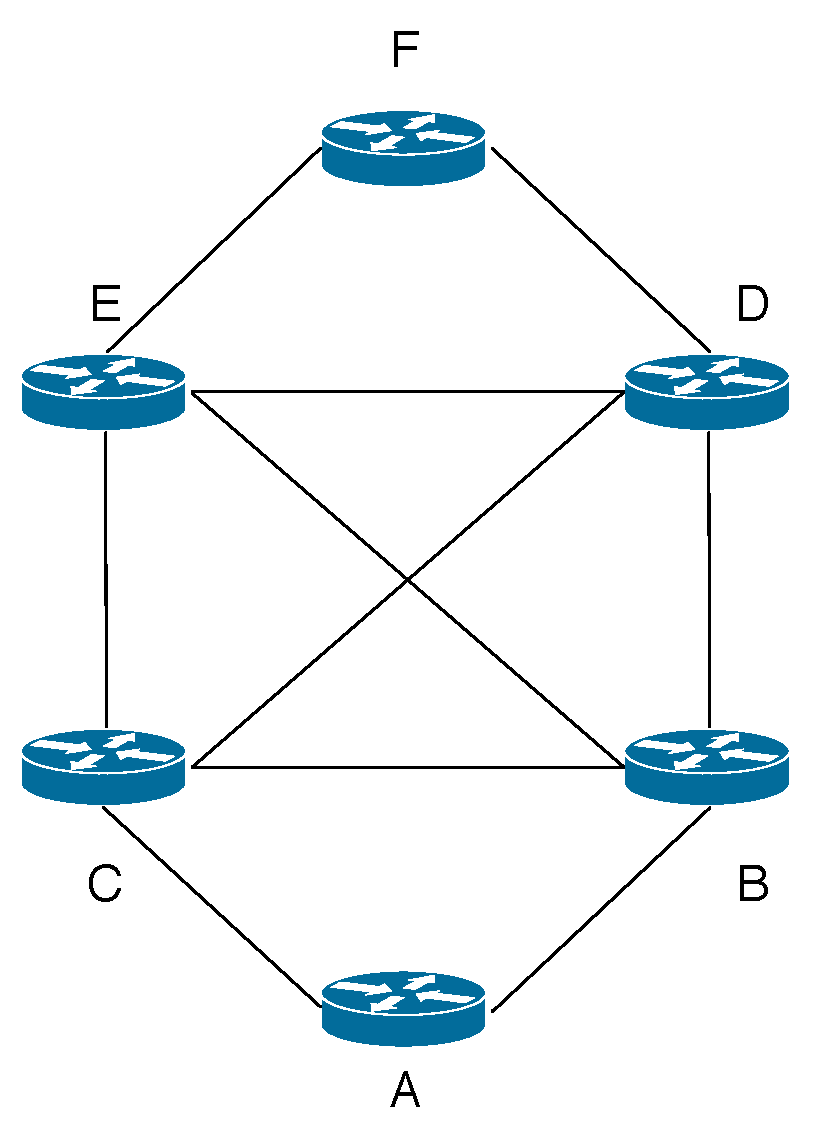
\includegraphics[scale=.75]{TestBed}
\caption{The reference topology.}
\label{fig:testbed}
\end{figure}

 
\subsection{The Classical - MultiRoute}

The classical implementation of MultiRoute is based on a single bit representation of congestion, which allows it to leverage local and remote congestion information. It is based on an approach similar as the one used in Random Early Marking \cite{REM} (REM). 

\subsubsection{Protocol Detail}

As stated above, MR is modeled on REM. Each router probabilistically marks a link as congested, this congestion information is then sent to neighboring routers allowing them to modify their route selection algorithm. Links are marked congested following an exponential measure of the link congestion (ie. the transfer function), doing so ensures that the marking probability is also exponential for the path congestion measure.

Achieving the behavior described above requires that each router to obtains both the
available paths for routing and their associated statistics. Conveniently, the
Path Discovery algorithm described in Section \ref{sect:MRPC} delivers
MultiRoute (MR) \cite{MR} with a set of valid multipaths available for
routing. Based on this set of links, MR builds a preliminary routing table
indicating the set of paths available for each destination. This, then, allows
MR to construct the \textit{Routing Mask} (shown in Figure \ref{fig:RM})
representing the structure used by the congestion updates. The local and remote
congestion information received from neighboring routers allows the current
router to build the final routing table which only contains the best (in terms
of congestion) next-hop to all destinations. The algorithm by which this table
is built is detailed in Section \ref{sect:MRAlgo}. 

The update message received from a neighboring routers is compared to the
\textit{Routing Mask} obtained initially from that same router. By aligning the
\textit{Routing Mask} and the update message, as shown in Figure
\ref{fig:RMCompare}, it is clear to the current router how to interpret the
update message and therefore it is evident which paths for each destination
are congested. Thereby, enabling a simple method to compute the final
routing table. 

Actually, the final routing table can be pre-computed as all the information to determine the next-hop for each destination is available before packets to these destinations arrive. Pre-calculating the final routing table is justified by the fact
that in the worst case update messages will be received at one second intervals as
this is the minimal polling interval router support for counter updates \cite{YaTG}.
Moreover, it minimizes the flow setup time as the router now only needs to
perform a lookup in the routing table to obtain the best next-hop.

\ifigure{RMCompare}{0.5}{Comparing a \textit{Routing Mask} with its an Update Vector}{fig:RMCompare}
% Build figure of comparison between remote routing mask and associated update vector. 
%	show sections which identify networks RMCompare

MultiRoute's Monitoring Protocol delivers the MR with raw statistics from the interface counters. MR then uses the transfer function shown in Equation \ref{eq:MRTF} to compute a 1-bit probabilistic marking of the router-router links, where $\Delta$ is the difference between two consecutive counter values and $\Gamma$ is the capacity of the router-router link. Finally, $\Phi$ is a scaling factor set by the network operator. Basically, the larger this factor is the more probable a link will be marked.

 \begin{equation}
P[Link~is~congested] = 1 - \Phi^{-\frac{\Delta}{\Gamma}}
\label{eq:MRTF}
\end{equation}

As the link utilization ($\rho = \frac{\Delta}{\Gamma}$) increases, the
probability to mark the link increases exponentially, as shown in Figure
\ref{fig:MRTF}, where the dotted lines show the curve for different values of $\Phi$. The 1-bit marking is derived by random variable who value is compared to the output of the transfer function, if the random variable is smaller than the output of the function then the linked is marked as congested. The rational behind this is that we want to rapidly mark a link
as congested in order to shift traffic from it as early as possible. 

\begin{figure}[htbp!]
\begin{center}

\begin{tikzpicture}[scale=6.0, domain=0:1]
    \draw[very thin,color=gray,step=0.5cm] (-0.1,-0.1) grid (1.2,1.2);
    \draw[->] (-0.2,0) -- (1.2,0) node[below = 28pt, left=3pt] {$\rho = Link~Utilization$};
    \draw[->] (0,-0.2) -- (0,1.2) node[left = 28pt, below=5pt] {$\rotatebox{90}{Prob. to set congestion}$};
    \foreach \x/\xtext in {1/1}
      \draw[shift={(\x,0)}] (0pt,2pt) -- (0pt,-2pt) node[below] {$\xtext$};
    \foreach \y/\ytext in {1/1}
    \draw[shift={(0,\y)}] (2pt,0pt) -- (-2pt,0pt) node[left] {$\ytext$};

    \draw[color=black] plot[id=exp] function{(1 - 50**(-x))}
      node[above] {$f(\rho) = 1-\phi^{-\rho}$};

      \draw[color=black,dashed] plot[id=exp1] function{1 - 25**(-x)} ;
      \draw[color=black,dashed] plot[id=exp2] function{1 - 10**(-x)};
      \draw[color=black,dashed] plot[id=exp3] function{1 - 5**(-x)};
      \draw[color=black,dashed] plot[id=exp4] function{1 - 3**(-x)};

%     \draw[color=black] plot[id=exp2] function{4*(1 - 500**(-x/4))}
\end{tikzpicture}

\end{center}
\caption{The transfer function used in Classical MultiRoute.}
\label{fig:MRTF}
\end{figure}

Another factor that is important is the \textit{Routing Mask} length obtained
when using this transfer function with the classical implementation of
MultiRoute. Trivially, the \textit{Routing Mask} length, given in bits, is shown
in Equation \ref{eq:MRRMLength}. 

\begin{eqnarray}
 RM~Length &=& (N-1) + N\displaystyle\sum\limits_{i=1}^N \frac{C_{i}}{N} \nonumber \\
&=& (N - 1) + N\bar{C} \nonumber \\ 
&=& N(1 + \bar{C}) - 1
\label{eq:MRRMLength}
\end{eqnarray}

Equation \ref{eq:MRRMLength} gives the derivation of \textit{Routing Masks}
where $N$ is the number of networks, $C_{i}$ is the number of uplinks per
destination. It is difficult, if not impossible, to predict the $C_i$ values as
they are linked to the topology therefore we define $\bar{C}$ as the average
number of uplinks per destination which is equal to the sum of $C_{i}$ divided
by $N$. The first term, $(N-1)$, represents the number of separator bits in
terms of number of networks and the second term represents the number of bits
required to represent the congestion per destination. Based on this equation we
have the 3D plot in Figure \ref{fig:MRRM3D} of the length of the \textit{Routing
Mask} as a function of the average number of uplinks and the number of networks.

\ifigure{RMLength}{0.5}{\textit{Routing Mask} Length as a function of $N$ and
$C$.}{fig:MRRM3D}


\subsubsection{Features and Limitations}

MR provides an extremely lightweight mechanism to represent congestion within a
multipath network. The crucial information describing which link to which
destination is congested is maintained by the Update Messages relying on the
\textit{Routing Masks}. Therefore, rather than aggregating congestion
information at each router, MR provides congestion information for each
router-router link and represents them clearly to all routers in the network
using a single bit. Due to the use of only a single bit to represent congestion,
MR is best suited for networks in which flows are long-lived and each flow
consumes the entire bandwidth offered by the router-router link. 

Moreover, MR uses a minimal amount of processing power at flow setup time as it
pre-computes the best next-hop for each destination. The selection algorithm
which builds the final routing table requires itself few resources. First, it
does not create any extra data structures, thereby requiring no extra memory.
Second, it is essentially a comparison algorithm and the elements of the
comparison are delivered in a simple form (Update Message). Therefore the
computation is
straightforward as shown in Section \ref{appdx:MR}. Overall, the  protocol
maintains just one extra table more than legacy protocols (such as
Shortest Path protocols). All protocols maintain a
routing table which contains the next-hop to any destination, MR also maintains the
preliminary routing table which contains all the possible paths to any
destination obtained from the path construction component.

As MR functions by receiving signals from neighboring routers, it is clear that
the main problem is the signal propagation time. Due to the congestion on the
paths, signals may either be delayed significantly or in the worst case, lost.
MMP, which is responsible for delivering the monitoring messages, does not
verify if messages arrive at their destination (thereby behaving like UDP). As
congestion increases, the probability to delay or lose packets increases
significantly but as MR monitoring messages only contain an Update Message
plus an MMP packet header they are very small (typically less than 200 bits as
shown in Figure \ref{fig:MRRM3D}). Therefore, the risk of delaying or losing
packets is mitigated by the size of the packets themselves. 

Another limitation is given by the \textit{Routing Mask} length itself. It is
known that the Maximum Transmission Unit (MTU) for an IPv4 path is 576 bytes,
and the MMP protocol does not support fragmentation\footnote{Moreover,
fragmentation is nowadays considered harmful \cite{FragBad}}. By setting \textit{RM Length} to
$576 * 8$ bits in Equation \ref{eq:MRRMLength}, we can see that there is an
inverse relationship between the number of networks and the average number of
uplinks per destination as shown in Figure \ref{fig:LenLim}. Considering that MR
is an interior-gateway routing protocol, an unreasonably large number of networks
and/or parallel uplinks would be required to exceed the MTU limit. 


 \begin{figure}[htbp!]
 \begin{center}
 
 \begin{tikzpicture}[scale=0.2, domain=0:46]
     \draw[very thin,color=gray,step=2] (-0.1,-0.1) grid (51,51);
     \draw[->] (-0.2,0) -- (52,0) node[below = 28pt, left=3pt] {$\bar{C}$};
     \draw[->] (0,-0.2) -- (0,52) node[left = 35pt, below=7pt] {$N$};
     \foreach \x/\xtext in {10/1000, 20/2000, 30/3000, 40/4000, 50/5000}
       \draw[shift={(\x,0)}] (0pt,2pt) -- (0pt,-2pt) node[below] {$\xtext$};
     \foreach \y/\ytext in {10/10, 20/20, 30/30, 40/40, 50/50}
     \draw[shift={(0,\y)}] (2pt,0pt) -- (-2pt,0pt) node[left] {$\ytext$};
 
     \draw[color=black] plot[id=line] function{(4608/(1+x))/100};
 
 %     \draw[color=black] plot[id=exp2] function{4*(1 - 500**(-x/4))}
 \end{tikzpicture}
 
 \end{center}
 \caption{Plot of the \textit{Routing Mask} Limitation}
 \label{fig:LenLim}
 \end{figure}
% PLOT 577*8/(1+C)!!! IN TKZ

  % Signal propagation time
  % Routing Mask length.
  % return path is itself extremely congested however this is mitigated by size.
      % as packet loss probability increases with congestion direct from queue.
% marks links as congested too early

\subsubsection{Routing Algorithm}
\label{sect:MRAlgo}

The Routing Algorithm in MR, given all the congestion indications, constructs the best (or least congested) next-hop based on the set of available paths obtained from the preliminary table. The pseudocode is given in Section \ref{appdx:MR}. The Routing Algorithm considers both local and remote congestion information and we distinguish three cases in which the algorithm operates:

\begin{itemize}
 \item \textit{Case I - All local paths uncongested.} In this case, we consider the remote congestion statistics relevant to the destination under consideration. If there are multiple local paths available, for each potential next hop the number of uncongested paths are counted. The local path associated to the next hop with the least congested paths is selected, thereby maximizing the probability that the traffic will be forwarded unhindered. On the other hand, if all the remote congestion counts are equal or if there are multiple candidates, the shortest path is selected.
 \item \textit{Case II - Some local paths are congested while others are not.} Here we first consider the uncongested local paths in ascending path lengths. Then the associated remote paths are inspected, if one is found that is not congested then it is selected as a next hop. Otherwise, the shortest path is selected. This case will attempt to fill available and uncongested paths, thereby increasing the overall throughput of the network.
 \item \textit{Case III - All local paths are congested.} In this last case, we perform a search which is similar to the first case. The idea being that we want to find a path that is well suited to accommodating more traffic. If none is found, we select the shortest path again.
\end{itemize}

It is clear from the outline of the algorithm that in the worst case the algorithm will always select the shortest path. Moreover, the algorithm favors the shortest path first, and only once this path is considered congested does the algorithm switch to an alternative path. This approach guarantees that the algorithm cannot perform worse in terms of throughput than the current shortest path algorithms.

Consider now the network shown in Figure \ref{fig:testbed} and the associated routing table given in Table \ref{tab:matrix}, and multiple flows originating from the network under router F with destination network at router A. For the purpose of this example, let us assume that the flow's inter-arrival time at the source router is greater than the update interval at neighboring routers\footnote{In practical terms, these routers poll their local statistics at one second intervals, therefore the update time is one second plus the update message transmission time.}. We also assume that each flow is long lived and immediately consumes the entire bandwidth of the path it utilizes. There are four paths between networks F and A, namely F-D-B-A (1), F-D-C-A (2), F-E-C-A (3), and F-E-B-A (4), path (1) is considered to be the shortest followed by path (2) and so on. As there are only two distinct paths we can expect to double the network throughput with respect to a shortest path algorithm.

When the first flow arrives, it is bound to path (1) as this path is considered to be the shortest, and due to Case I, this then causes an update from the routers F, D, and B indicating that their links are congested. When the next flow arrives, the decision is taken by Case II of the algorithm, and therefore the algorithm will consider the paths with next hop E as this link is not congested. The path (4) is excluded, because the link between B and A is congested due to the first flow. Therefore the second flow is bound to path (3). Finally, for each subsequent flow, Case III of the algorithm will apply. The next two flows will be bound to paths (2) and (4) respectively, and the rest will be sent along the shortest path.

\subsection{The Organizer - StepRoute}

StepRoute \cite{SR} is a variant of MultiRoute which enables the network administrator to
define congestion classes. These classes allow for a finer control of the
congestion of the network and therefore enable for a more efficient use of the
network resources.

\subsubsection{Protocol Detail}
\label{sect:SRDetail}

StepRoute contrasts with MultiRoute by first extending the \textit{Routing Masks} to accommodate the definition of congestion classes. Second, it uses a linear transfer function rather than an exponential one in order to simplify the definition of the congestion classes. Based on a predefined value, a link is deemed to be part of one of the congestion classes. 

By classifying congestion into classes and using \textit{Routing Masks}, we are able to deliver timely information to routers while maximizing the accuracy of the delivered statistics. Each router has to define the same number of congestion classes, otherwise neighboring routers will not be able to interpret the \textit{Routing Masks} received correctly.  

 \begin{equation}
\gamma = \frac{\Delta}{\Gamma}
\label{eq:SRTF}
\end{equation}

In a similar fashion to MR, StepRoute obtains its raw statistics from MMP.
StepRoute then classifies the link into the corresponding congestion class based
on the transfer function, shown in Equation \ref{eq:SRTF}, and the congestion
classes defined in Table \ref{tab:CongClass} where the $\alpha$ values are the congestion class boundary value. As the link utilization increases
the link is classified into a higher congestion classes, thereby simplifying the
process by which the Routing Algorithm will select the next-hop, ie. favor
links in lower congestion classes.

\begin{table}[h!]
  \begin{center}
    \begin{tabular}{| c || c |}
\hline
 Class 1  & $ 0.0 < \gamma \leq \alpha_1$ \\
 Class 2  & $ \alpha_1 < \gamma \leq \alpha_2$ \\
 Class i  & $ \alpha_{i-1} < \gamma \leq \alpha_i$ \\
 Class P  & $ \alpha_{P-1} < \gamma \leq \alpha_P = 1.0$ \\
\hline
    \end{tabular}
  \end{center}
  \caption{Congestion Classification.}
\label{tab:CongClass}
\end{table}

Figure \ref{fig:SRTF} depicts the linear transfer function used in StepRoute. In
this variant of MultiRoute, it is preferable to use a linear transfer function
as we wish to distribute traffic equally amongst all the links we have at our
disposal. If an exponential transfer function had been used then links would
quickly fall into the highest congestion class and links with unused
bandwidth would not be used. 

\begin{figure}[htbp!]
\begin{center}

\begin{tikzpicture}[scale=6.0, domain=0:1]
    \draw[very thin,color=gray,step=0.5cm] (-0.1,-0.1) grid (1.2,1.2);
    \draw[->] (-0.2,0) -- (1.2,0) node[below = 28pt, left=3pt] {$\rho = Link~Utilization$};
    \draw[->] (0,-0.2) -- (0,1.2) node[left = 28pt, below=5pt] {$\rotatebox{90}{Congestion Value}$};
    \foreach \x/\xtext in {1/1}
      \draw[shift={(\x,0)}] (0pt,2pt) -- (0pt,-2pt) node[below] {$\xtext$};
    \foreach \y/\ytext in {1/1}
    \draw[shift={(0,\y)}] (2pt,0pt) -- (-2pt,0pt) node[left] {$\ytext$};

    \draw[color=black] plot[id=linear] function{(x)}
      node[above] {$f(\rho) = \rho$};

     
%     \draw[color=black] plot[id=exp2] function{4*(1 - 500**(-x/4))}
\end{tikzpicture}

\end{center}
\caption{The transfer function used in StepRoute.}
\label{fig:SRTF}
\end{figure}

Using such a classification mechanism we can simply encode the congestion class
number in the Update Message. Therefore if we would like to represent $m$
classes of congestion where $m$ can be expressed as $2^{n}$, then we only need
$n$ bits per router-router link are needed to represent all the congestion
classes. Therefore, as the number of congestion classes grows exponentially, the
space required to represent them, in the Update Message, grows linearly.
This method allows us to describe
many congestion classes while employing a lightweight, and therefore easily
distributable, representation.


%\begin{figure}
%\begin{center}
%\begin{tikzpicture}[scale=0.5, domain=0:4]
%    \draw[very thin,color=gray] (-0.1,-1.1) grid (3.9,16.9);
%    \draw[->] (-0.2,0) -- (4.2,0) node[right] {$n (bits)$};
%    \draw[->] (0,-1.2) -- (0,17) node[above] {$f(n)$};
%    \draw[color=black] plot[id=2x] function{2**x} 
%        node[right] {$f(n) = 2^{n}$};
%\end{tikzpicture} 

%\end{center}
%\caption{The number of congestion classes representable per X bits}
%\label{fig:classes-explin}
%\end{figure}

On the other hand, using multiple bits to represent the congestion class will require longer \textit{Routing Masks} as each entry for each destination in the \textit{Routing Mask} is now $n$ bits long.  We therefore have Equation \ref{eq:SRRMLength} which represents the length of the \textit{Routing Masks} in StepRoute. 

\begin{eqnarray}
 L &=& (N-1) + N\displaystyle\sum\limits_{i=1}^N \frac{nC_{i}}{N} \\
&=& (N - 1) + Nn\bar{C} \\ 
&=& N(1 + n\bar{C}) - 1
\label{eq:SRRMLength}
\end{eqnarray}

Equation \ref{eq:SRRMLength} is identical to Equation \ref{eq:MRRMLength} if we
set n, the number of bits required to represent the congestion classes, to one.
Therefore, all the other terms in Equation \ref{eq:SRRMLength} represent the
same thing as for MR.

%%%% 3d FIGURE OF ROUTING MASKS!!! FROM MATLAB!! <- NOPE!

\subsubsection{Features and Limitations}

As StepRoute is built on top of MultiRoute it inherits all the functionality that MR had, but also it also suffers from the limitations of MultiRoute. Namely, it suffers from the same problem of signal propagation time and the potential \textit{Routing Mask} length. Due to the fact, that StepRoute uses more bits in the \textit{Routing Masks} than MultiRoute, it supports less networks or less connections per destinations. In other words, the inverse relationship between number of networks and number of connections in StepRoute is steeper than in MultiRoute.

StepRoute uses slightly more memory than MultiRoute as it requires three tables. The first two are also found in MultiRoute, the third table is used to convert the raw congestion value into a congestion class. The size of this table depends entirely on the number of congestion classes and therefore it is safe to say that it contains $n-1$ entries.

StepRoute allows for a finer control of the congestion on the network. By
defining multiple congestion classes, StepRoute can represent the current level
of congestion to neighboring routers and therefore attempt to install flows onto
paths which have enough bandwidth to support the new flow. This approach leads
to much better usage of the network resources especially in the presence of
flows which do not consume the entire bandwidth of router-router links.
Typically, if the the router uplinks have a much larger capacity than the
underlying network, StepRoute will load balance this traffic much more
efficiently than MultiRoute, as flows will always consume a fraction of the
capacity of the uplink and therefore the congestion classes will describe more precisely the partial congestion present on each uplink.

%%RETHINK CONCLUSION!

\subsubsection{Routing Algorithm}

Similarly to MultiRoute, StepRoute distinguishes three cases which represent the state of the congestion local to the router. Then, based on these three cases it selects the current best next-hop from the preliminary routing table and constructs the final routing table.  The pseudocode is given in Section \ref{appdx:SR}. We should note here that the algorithm considers the lowest congestion class as already being congested and therefore attempts to avoid the potentially lightly loaded link.

\begin{itemize}
 \item \textit{Case I - All local paths uncongested.} In this case, the
algorithm only looks at the statistics received from neighboring routers.
Assuming there are multiple paths available, the router searches for the least
congested path which is simple due to the classification of the congestion
values discussed in Section \ref{sect:SRDetail}. Clearly, if the
algorithm finds a remote path with is not at all congested, it immediately
selects this path for forwarding. On the other hand, if all the remote
congestion counts are equal or if none is found, the shortest path is selected.
 \item \textit{Case II - Some local paths are congested while others are not.}
This case is slightly more complex because a local path, even if it is carrying
some traffic, may still be amongst one of the better options. This is due to
the fact that remote paths, which lay beyond a completely uncongested link, may
be completely congested. In this case, the algorithm ranks the candidate paths
by summing their local congestion with the remote congestion. The path with the
lowest congestion value is then selected. As with Case I, if there are multiple
candidates, the shortest one is selected.
 \item \textit{Case III - All local paths are completely congested.} This case
is very much similar to the first case. The idea here is to look at the
congestion values of remote routers and determine the least congested path, in
an effort to use up all the available bandwidth. Again, if multiple candidates
are found, the algorithm defaults to the shortest path.
\end{itemize}


Let us consider, as an example, the network given in Figure
\ref{fig:testbed} and its associated Table \ref{tab:matrix}, when multiple
flows enter at router F destined for network A. We also assume that each flow is
long lived  and that it immediately consumes half of the available bandwidth.
There are four paths between networks F and A, namely F-D-B-A (1), F-D-C-A (2),
F-E-C-A (3), and F-E-B-A (4), path (1) is considered to be the shortest followed
by path (2) and so on. As there are only two distinct paths we can expect to
double the network throughput with expect to a shortest path algorithm. It is
important to note that, with respect to the real implementation the routing
tables are pre-computed as statistics become available and not when a flow
arrives.

When the first flow arrives, it is bound to path (1) as this path is considered
to be the shortest, and due to Case I, this then causes an update from the
routers F, D, and B indicating that their links are partially congested. When
the next flow arrives, the decision is taken by Case II of the algorithm, and
therefore the algorithm will consider the paths with next hop E as this link is
not congested. The path (4) is excluded, because the link between B and A is
congested due to the first flow. Therefore the second flow is bound to path
(3). Upon arrival of the third flow, Case II will rank the available paths
according to the congestion level and will choose path (2) as the link between
D and C is not congested. Similarly, when the fourth flow arrives, Case II
ranks the available paths again and picks path (4). As subsequent flows arrive
at router F, Case III attempts to find available bandwidth to send the flow on
and if this is not possible it sends it onto the shortest path.


Similarly to MultiRoute, the algorithm defaults to the shortest path as well. This default is to reduce the delay experienced by the packets in the situation where no best option exists. 
  

\subsection{The Know-it-all - PathRoute}

While MultiRoute provides a link by link measure of the path congestion, PathRoute provides the actual congestion over the entire path from a given source to any destination. MultiRoute could in certain circumstances lead traffic into a congested area of the network due to a lack of knowledge of the effective distant congestion. PathRoute, by reporting entire path congestion at every router, avoids this situation and will never lead traffic into a congested area to the extent of the possible of course. 

While the previous two protocols limited themselves to distributing update
vectors to their direct neighbors only, PathRoute concatenates the information
contained in update vectors to deliver the path congestion for each router. To
achieve this objective PathRoute uses the same transfer function as MultiRoute
and also represents congestion on a single bit. The difference resides in the
fact that now the protocol analyzes the information received from its neighbors
to derive the path congestion. In order to distribute path congestion, 
PathRoute needs to know two pieces of information:

\begin{enumerate}
\item The set distances from a given router to all the other routers in the network. This will allow PathRoute to define the length of the \textit{Routing Masks} and therefore construct the initial mask which will be used to inform neighboring routers about the structure of the update messages.
\item The set of congestion information that should be concatenated at each
router and sent to neighboring ones.  A router needs to determine which part of
an update message is relevant to it, then concatenate this information and send
it to neighboring routers.
\end{enumerate} 

The first problem is solved using Diffusion Algorithms with termination
detection \cite{DijkstraTerm}. Each router initiates a computation by outputting
an Update MMP of code INIT on each of its router-router links for each destination and
keeps track of the number of messages it has sent and received. Next, when a
router receives an Update MMP with code INIT, it checks whether the packet is
destined for it, if it is then the router increments the distance counter
(contained in the packet), changes the code of the packet to NEW and replies to
the source over the shortest path. Otherwise, the counter is incremented and the packet is forwarded to the
destination, if the current router has multiple paths to the destination it
duplicates the packet and sends it down each of the uplinks for that
destination. Then, if a router encounters an MMP with NEW code, it checks
whether its number of sent and received messages is equal, if yes it sends the
reply towards the source along the shortest path otherwise it simply stores it.
Doing so, guarantees that if router sends a reply it is either the destination
of the query or it has received as many queries as it has sent and therefore by
the time the source obtains a reply we know that the computation has terminated.
Finally, when the source receives a reply it updates its distance table. The
flowchart in Figure \ref{fig:distflow}. Once all the routers have computed their
relative distances, each router can now construct and send their \textit{Routing
Mask} to their neighbors. This process occurs at the initial state of the network and therefore we assume that no other traffic can interfere with this process. 

%%FLOW CHART DIFF COMP & figure of aggregation...
\ifigure{DistFlow}{0.4}{Flowgraph of the distance diffusion computation.}{fig:distflow}

The second issue can be divided into two sub-problems. First, knowing that each
entry for a destination in the Update Message contains the entire path
congestion to that destination, the protocol must first know where to insert its
local congestion information. Second, when receiving an update message the
router must identify the parts of the update message which are of interest to
it, ie. the parts which describe the congestion to one or more of its
destinations.

The first sub-problem can be solved quite easily. Knowing the distance and the
number of uplinks for any destination, given by the distance table and the
preliminary routing table respectively, the router can easily identify the first
bit of a path description which will be the congestion value for its local
uplink.  The following sub-problem relies on the structure of the
\textit{Routing Mask}. When a router receives an update message, it first
determines if the port on which the message is received is used for any
destination and if so, is the distance to the destination on this port greater
than one? Then by comparing the message with the \textit{Routing Mask}, just
like in MultiRoute or StepRoute, it determines which parts of the update
message contain information about one or more of its destinations. The router
can simply copy the interesting parts of the update message into its own update
message, by concatenating the local congestion on the uplink with information
received in the update message from the neighbor. This new update message is
then propagated to the neighbors which therefore distributes the congestion
information around the network and enables routers to build their view of the
path congestion. This process is referred to as the aggregation step of
PathRoute. 

The major side-effect of representing the entire path congestion within the update messages is that their length increases significantly. While this is intuitively trivial, it is not so clear analytically since it is impossible to formalize the path length as it is intimately coupled to the network topology. Therefore  we can only predict the message size by specifying an average path length, $\bar{P}$, as shown in Equation \ref{eq:PRRMLength}.

\begin{eqnarray}
 L &=& (N-1) + N\displaystyle\sum\limits_{i=1}^{N} P\frac{C_{i}}{N} \\
&=& (N - 1) + N\bar{P}\bar{C} \\ 
&=& N(1 + \bar{P}\bar{C}) - 1
\label{eq:PRRMLength}
\end{eqnarray}

\subsubsection{Features and Limitations}

PathRoute delivers an extremely space and computation efficient mechanism for representing the path congestion at each router. By computing the distance from any router to another, PathRoute is able to extend its \textit{Routing Mask} with space to describe every link along the path to a destination and therefore deliver full path congestion information to every router. Finally, since each router running PathRoute knows all the information about the status of the path to the destination, the resulting routing algorithm is very simple and only requires information which is locally stored which therefore enables rapid flow installation.

By design, MultiRoute may unknowingly route traffic into congestion since it only has congestion information about its local links and its neighbors links. Therefore, if congestion lies beyond the next-hop andthe next-hop has no other option then MultiRoute may exacerbate the congestion in some areas of the network. PathRoute, on the other hand having full knowledge of path congestion, will never route traffic into congestion unless there is no other option available to it. 

Even though PathRoute provides deep information about the status of the network to each router, it requires no more memory than StepRoute. Three tables  are required, a preliminary routing table, a final routing table, and a distance table. On the other hand, initially, PathRoute requires slightly more CPU power as it must send MMP packets to compute the relative distances from one router to another.

As PathRoute is built on top of MultiRoute, it suffers from the same problems. Moreover, since update messages may be aggregated, the propagation delay for an update message is potentially multiplied by the path length. Therefore, the probability of delay or drop of the update message is also increased, but again this is mitigated by the relatively small size of these messages. 

\subsubsection{Routing Algorithm}

As each router now has all the information about the path congestion, there is no longer a need to distinguish three cases for the routing algorithm. PathRoute's routing algorithm takes the simplest form. More precisely, it simply finds the least congested path and forwards packets through the associated next-hop. As shown in \ref{appdx:PR}, the routing algorithm is straightforward and simply counts the number of links which are not congested. The path which contains the least number of congested links is selected.

Consider, once again, the network given in \ref{fig:testbed} and its associated
connectivity Table \ref{tab:matrix}, when flows originate at multiple routers in
the network. Let us also assume that each flow directly consumes the entire
bandwidth proposed by the path. We assume that the source routers are F, D, and E and a single destination
A. Therefore, the available paths are F-D-B-A (1), F-D-C-A (2), F-E-C-A (3), 
F-E-B-A (4), D-B-A (5), D-C-A (6), E-C-A (7), and E-B-A (8). 

Considering the situation described above, two flows arrive at router F. Based on PathRoute the first flow will select path (1) and the second path (2). Now, a flow arrives at router D, since path (5) has now two congested links (D-B and B-A) caused by the first flow. Router D selects path (6) which only has one congested link. The same occurs for the flow that originates at Router E and path (8) is selected.  We can see that PathRoute will attempt to use all the links of the networks before sharing full paths.
	
\subsection{Implementation Experience}

The entire MultiRoute family was designed and implemented within NOX (see
Section \ref{sect:OPFW}). NOX is a controller API for OpenFlow whose main
advantage is the exposition of a simple API  which enables the rapid
prototyping of research networking protocols. NOX introduces the concept of
components which can be viewed as black boxes computing a certain function, for
example, compute the set of shortest paths within a network. NOX components
communicate via events and direct message passing.


The design of the MultiRoute family is based on components. Each function
described the previous section is implemented with a component. The component
itself may be further segmented into various files. The code which makes up the
MultiRoute suite is highly modular. Each protocol depends on different
components. Changing these components modifies the behavior of the protocol. For
example, switching the transfer function in MultiRoute for the one which
computes congestion classes yields the StepRoute protocol. Figure
\ref{fig:MRDeps} show the dependency maps for each protocol, notice that each
protocol differs only in some of the components used. Since similar components
expose identical API or produce the same events, most of the code from one
protocol to another is re-used. This design accelerates the implementation cycle
and guarantees that the code is stable from protocol to the next. Moreover, the
implementation was almost exclusively done using Python \cite{Python} which
means that the implementation itself was simple and is easily understandable.
  
\ifigure{DepMap}{0.5}{Inheritance/Dependency graph for MultiRoute-based protocols }{fig:MRDeps}  
  
%discuss modularity of the MR suite
% change behavior by simply changing transfer function
% change routing algorithm to change next-hop selection.
% Enables switching of protocol mid flight

\section{Commodity Protocols}

The protocols detailed below were implemented to enable us to test
MultiRoute-based protocols against the protocols which are used today in
industry. Each of these protocols were implemented on our OpenFlow-enabled
testbed.

%Protocol to test against...

\subsection{Shortest Path}

Shortest Path Routing is a direct application of Dijkstra's Shortest path
algorithm \cite{DIJK}. In essence, it is a destination-based, load-insensitive
routing algorithm which is built based either on the minimum hop count or sum of
link weights. Therefore, given a destination the routing algorithm performs a
lookup in its routing table, which contains the next-hops to every destination,
and returns the next-hop of the shortest path to the requested destination.

This protocol is made to resemble OSPF \cite{OSPF} as much as possible without
having to re-implement the totality of OSPF. This is justified, as we are only
interested OSPF's routing model but not its distributed nature nor all its
extra functionality.

\subsection{Equal Cost MultiPath}

Equal Cost MultiPath (ECMP) \cite{RFC2991} is similar to Shortest Path routing in
that it is also destination-based but it differs in the fact that multiple best
paths may be used to forward packets. Therefore, as it name indicates, if the
network contains multiple shortest paths between any source-destination pair
then they are all used to forward packets.

Normally, ECMP uses a hash which is computed based on the source and
destination mac-address contained in the packets. In our case, out network
testers and machines connected to our testbed only have a limited number of mac
addresses. Therefore, to increase the diversity of the hash, we have computed
based on the source and destination port numbers which are random for every
flow. 

Section \ref{sect:HTE} derives and explains the number of disruptions to expect
when a link of an ECMP set goes offline.

\section{Theoretical Delay Model for MultiRoute-based protocols}

In this section, we will use the model detailed in Section
\ref{sect:queues} to derive a delay model for Congestion-Aware Routing
protocols. Furthermore, we also evaluate the average number of flows present
at any node in the system.

A multipath network can be seen as a system with multiple servers. Each server,
therefore would represent an uplink between nodes in the system. Routers are
then referred to as nodes. We now need to define the arrival (input) and
departure (output) models. We can safely assume that the arrival model is
Markovian since packets sent are sent from end nodes (ie. computers) are independent
and memoryless, the same goes for the output model since it only depends on the
actual packet length of the router which is constant. Therefore we can model
our first queue in the System as M/M/m queue (see \ref{sect:mmmQ}). But, as explained
in Section \ref{sect:kleindep}, we cannot simply say the same thing for any
other queue in the system as the message length and the inter-arrival times
become highly dependant. Fortunately, Kleinrock's Independence assumption
\ref{th:indep} and in particular Burke's Theorem, allow us to select a new message size at the output of each
queue independently and therefore model our entire system as independent M/M/m
queues.

Therefore, we can now say that the delay created by a certain node is the
average time spent in the system and for an M/M/m queue is given by:

\begin{equation}
 T = \frac{1}{\mu}\left(1 + \frac{P_{Q}}{m(1-\rho)}\right)
\label{eq:Delay1node} 
\end{equation}

Where $P_Q$ is given by Equation \ref{eq:MMMPQ} and $\frac{1}{\mu}$ is the
service time and $\rho = \frac{\lambda}{m\mu}$ is the utilization ratio with
$\lambda$ the arrival rate and $m$ the number of servers.

Since, we claim that each queue is independent we can state that the overall
delay in the network is simply a function of the number of hops a packet must
traverse and therefore we have:

\begin{equation}
\bar{T} = \bar{n}T
\label{eq:overallDelay} 
\end{equation}

\ifigure{delay}{0.5}{Flow delay as function of the load
($=\frac{\lambda}{m\mu}$) and number of servers.}{fig:delay}

Figure \ref{fig:delay} shows that as the arrival rate increases the overall
load on the system increases and eventually leads to $\infty$ which is to be
expected because the expression for delay is dominated by $1 - \rho$

Another interesting quantity is the number of clients (ie. flows) that are
present at any queue. This quantity will allow us to determine the expected
disruption should a queue become unavailable for some reason.

\begin{equation}
 \bar{N} = m\rho + \frac{\rho P_{Q}}{1-\rho}
\label{eq:disruptions} 
\end{equation}


Since Equation \ref{eq:disruptions} is also dominated by $1 -\rho$, we would
have the same behavior than in Figure \ref{fig:delay}. Namely, as the system
load increases the number of flows in queue will increase as well. Figure \ref{fig:queuers} shows the number of flows waiting at each queue. We can see that as the arrival rate increases, the number of flows in the queue increases significantly. This value can also be seen as the number of flows that would be disrupted if an uplink where to go offline, thus giving us an approximation on the number of communications that would need to be re-established should there be a problem. We should note that if we pick $m=1$, then we have a model for a single path system. We can see that in such a system the delay increases significantly than in multipath systems.

\ifigure{queuers}{0.25}{Number of flows in each queue}{fig:queuers}

\section{Summary}

%Your final comment: "this seems like it missed a bit. OK, time I got here I had forgotten where it started but if I look back to the intro you talk about RFC xyz which never gets another mention. Also if the IS where you mean to end then what was the value of what you just described? Latency increases with load...nothing new there. More flows per queue as the load goes up, hmm, I don' follow, seems to me its a question of how many flows AND what their relative weights are and assuming I'm wrong, as usual then what is the conclusion: the more traffic you have the more you are fucked when one route shuts down? That's not exactly rocket science is it?  "

%You are right, I completely skipped the summary, probably cos I got bored... The point of all this is to say that while nothing super new occurs when you use multipaths, you still get more delay as the load increases, queues get more and more full and so on, but all this happens later that in the single path model. More importantly this happens later even if you coarse route (as in route by flow and not packet by packet). In itself, this a nice discovery because it means that if we route flow by flow we can still expect significant gains over single path techniques.

In this section, we have described three protocols by using the outline given in RFC 1264 \cite{RFC1264} then we gave several theoretical predictions which, while not fully accurate, provide us with an idea  of the performance we can expect of our protocols. 

The first protocol, MultiRoute, describes congestion as a single bit. While the second, StepRoute, defines congestion classes. Finally the third protocol, provides a congestion measure for the entire path from source to destination.

Using multipaths does not change the rules of the game in networks, by this we mean that the latency still increases as the load on the network increases and queues still get more and more full as the load increases. That said, all these phenomena happen when the load is higher than in the single path settings. More importantly, we also see that even though each of our protocols routes flow rather than individual packets, we can still expect a significant increase in performance while not optimal it is still quite a desirable increase over single path routing.  

%Based on previous chapter. Plot explain derivation and plot theoretical delay
% and number of flows at each node (if it makes sense).



\chapter{Materials \& Methods}
\label{chap:materials}

\begin{flushright}
 \textit{\textquotedblleft If you are afraid of change,
leave it here.\textquotedblright}\\
\textit{-- Seen on a tip box, Mountainview, CA}
\end{flushright}

\ifpdf
    \graphicspath{{6-MaterialMethods/Chapter6Figs/PDF/}}
\else
  \graphicspath{{6-MaterialMethods/Chapter6Figs/}}
\fi

\section{OpenFlow \& NOX}

OpenFlow is an open standard which enables a network engineer to control the behavior of their networking equipment programmatically. It represents a radical shift for the networking status quo. First,
manufacturers need to embrace OpenFlow and implement it\footnote{So far, HP,
NEC and Broadcom are known to have hardware implementations.}. Second, it
signals the end of distributed network algorithms and a return to simpler
centralized algorithms. 

OpenFlow and NOX are the basis for the implementation of the work in this Thesis. While the author believes that the future of computer networks lie alongside OpenFlow, he has implemented his work in a distributed manner in order to resemble current day network protocols.

\subsection{OpenFlow}
\label{sect:OPFW}

OpenFlow \cite{OPFW} offers a way for network researchers to try their
experimental protocols on real hardware and on the networks they use every day.
Until now there has been an extremely high barrier to entry for new networking
ideas due to the face that there is a rational reluctance within the community
to experiment with production traffic. The installed base of networking hardware has been largely built to conform with the extant RFC's and as such offers few, or no external interfaces. The result of this has been to exclude innovation since there is no mechanism to deploy or test alternative strategies to the ones laid down in silicon. Up until quite recently the only way that experimental progress could be made was work with specific experimental installation such as GENI \cite{GENI}. GENI is an nation-wide
(in the United States) network which provides programmable network elements via
virtualization and is capable of processing packets for multiple isolated
experiments. The disadvantage with such installations is that they are very
costly and take years to implement. Another example of such systems, while
smaller, are Emulab \cite{Emulab} and StarBed \cite{StarBed}.

There also exists several software solutions. Many OSs can route packets between
their interfaces and software implementation of routing protocols exist, for
example from XORP \cite{XORP} (eXtensible Open source Routing Platform).
Moreover, the CLICK \cite{CLICK} router project allows researchers to control
and manage the packet processing. While these solutions are interesting, they
do not provide the performance  or the port density required to test news ideas
efficiently. Hardware implementations are also available, the largest one is the
Advanced Telecommunications Computing Architecture Supercharged PlanetLab
platform \cite{PlanetLab} but it is targeted for large deployments and it is
extremely costly. There is also a NetFPGA \cite{NETFPGA} solution, but this
only provides four ports per card.

The question is why can we not find a way to use the hardware we
currently have and the networks we have deployed. This is exactly what OpenFlow
is designed to do.


\ifigure{Ofsign}{0.7}{The OpenFlow flow signature.}{fig:flowsign}

OpenFlow exploits the flow-tables contained in modern switches. Flow-tables are
built from TCAMs\footnote{A TCAM is a Ternary Content Addressable Memory. This
allows the operating system to match a third state, "X." The X state is a
"mask," meaning its value can be anything. This lends itself well to networking,
since netmasks operate this way. Routers can store their entire routing table in
these TCAMs, allowing for very quick lookups.}, which allow functions like QoS,
NAT, firewalls to run at line rate. OpenFlow stores the signature of a flow,
shown in Figure \ref{fig:flowsign} into the flow-table, and associates one or
more actions to be applied to the flow. The signature then allows the switch
to match subsequent packets onto that flow. The overall effect of the actions 
determines the behavior of the network. Figure \ref{fig:openflow} shows an
OpenFlow-enabled switch which is made up of a secure channel and a flow-table.
The secure channel connects the controller to the switch enables the controller
to send commands to the switch and manipulate its flow-table.

\ifigure{openflow}{0.5}{The OpenFlow switch.}{fig:openflow}

OpenFlow then provides an open and programmable interface to control the
contents of the flow-table. The set of actions which can be applied depend on whether
the switch implements all the actions or only the required ones. Moreover,
some manufacturers may not be able to implement certain actions due to their
underlying hardware as we will see in Section \ref{sect:NetHard}. The set of 
actions supported by an Openflow switch are summarized below:

\begin{itemize}
\item \textbf{Set VLAN ID} - Specify or overwrite the VLAN identifier.
\item \textbf{Set VLAN priority} - Define the priority of the packet with the VLAN.
\item \textbf{Strip VLAN header} - Remove all VLAN information.
\item \textbf{Modify source or destination MAC address} - Overwrite the Ethernet header information. 
\item \textbf{Modify source or destination IP address} - Overwrite the IP header information.
\item \textbf{Modify ToS bits} - Modify the Type of Service bits.
\item \textbf{Modify Transport source or destination ports} - Overwrite the TCP header information.
\end{itemize}

OpenFlow decouples the control from the datapath and exports it to a
controller, such as NOX, which will control the contents of the flow table. As an OpenFlow device is usually referred to as a switch even though technically it is not a stereotypical switch. OpenFlow can implement the function of a switch, router or even both; but it may also implement any other function. The term switch here is used to refer to the hardware on which OpenFlow is deployed.

\subsection{NOX}

NOX \cite{NOX} is an OpenFlow controller whose goal is to provide a programmatic
interface so that other applications can manage the underlying network. NOX
presents applications with a centralized programming model. NOX, programs are
written as if the network were contained on a single machine. NOX abstracts
low-level network details away from the developer. It essentially provides a
framework to manage OpenFlow-enabled switches and routers by handling the
low-level OpenFlow API provided by the enabled hardware.
 
A NOX based network is made up of openflow-enabled switches and one or more
instances of NOX where each instance provides the exact same network view to
the developer(s). Network applications are written on top of NOX and control
the behavior of the network by manipulating the flow-table. During normal
operation, NOX receives flow initiations (first packet of an unmatched flow),
these are passed by NOX to the network application which decides what to do
with such a flow. In the end, a new flow rule may be added to the flow table
and therefore subsequent matching flow will not be sent to NOX but rather the switch will apply the action specified in the added flow rule.

NOX's programmaable interface is driven by events, the namespace and the network
view. Traffic patterns in modern networks are constantly shifting therefore
flows come and go, links go up and down. NOX handles this by allowing developers
to register for events. When an event occurs NOX calls the handler passed at
the registration. 
  
NOX builds a network view based on messages obtained from the Openflow-enabled
switches as they connect. Applications use the network view to perform
computations or decide how to handle a certain type of packet, etc. Each NOX
instance constructs a list of loaded applications and from this point onwards
each loaded application can exchange messages with each other. This is known
as the NOX namespace. 
	

\section{TestBed Installation}

\subsection{Routing Hardware}
\label{sect:NetHard}

The testbed is implemented on HP Procurve switches [procurve] running an
experimental OpenFlow-enabled firmware. OpenFlow on the HP platform is
instantiated per VLAN\footnote{Virtual Local Area Network}. We have exploited
this by defining different VLANs on each network device which are then used to
identify the network address range controlled by the device. The VLAN ID is
then advertised to the controller who uses it to assign a virtual gateway
address for each router in the network. 

The HP implementation of OpenFlow has several limitations which are mostly due
to the underlying hardware. For example, HPs cannot perform mac address
rewriting in hardware because their routing support is monolithic and the
re-writing functionality cannot be isolated from the other routing
functionality. It is actually more limiting, HPs can only re-write mac-addresses
to a single mac address (the base address of the device) and therefore
specifying a custom mac address is impossible. Since the hardware does not
support some OpenFlow actions, they are implemented by the OpenFlow firmware in
software. As the processor within switches is a shared resource between all the
ports and is not very powerful in the first place, the software path is a
very slow path. Our measurements show that the software path provides roughly
1.25 MB/s overall bandwidth per switch, this is equivalent to 10Mb/s cross
sectional bandwidth. 

Since we are designing a new routing protocol which is supposed to surpass all
existing ones in terms of performance, using our OpenFlow devices in software
path (ie. invoking the switch CPU) is counter productive. Therefore we have employed several workarounds in
order to build a routing protocol using HP's OpenFlow implementation.

\begin{figure}
  \centering
  \subfloat[Standard routing model.]{\label{fig:normalrouting}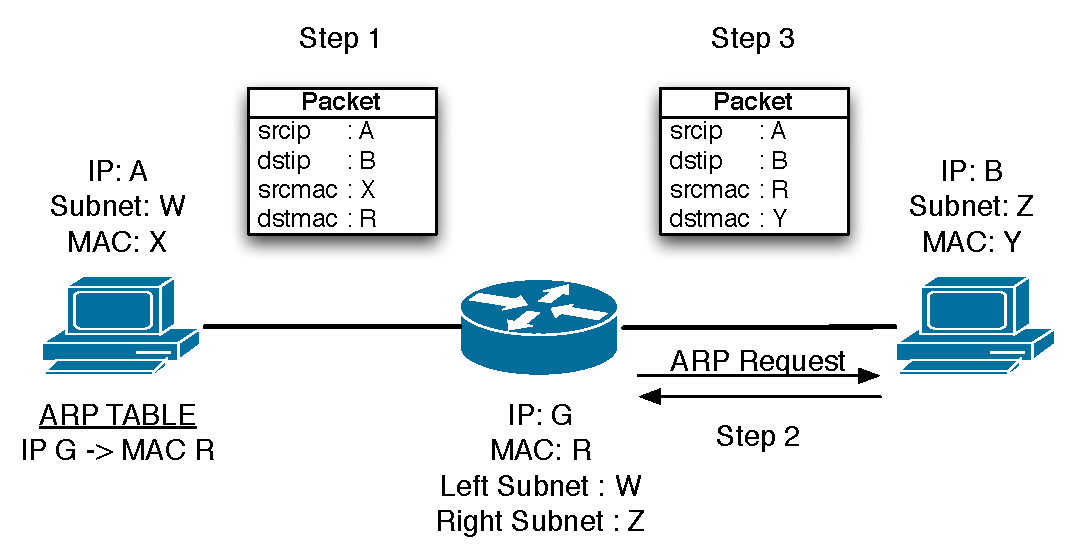
\includegraphics[width=\textwidth]{normalrouting}}
  \\                
  \subfloat[HP Openflow Routing.]{\label{fig:HProuting}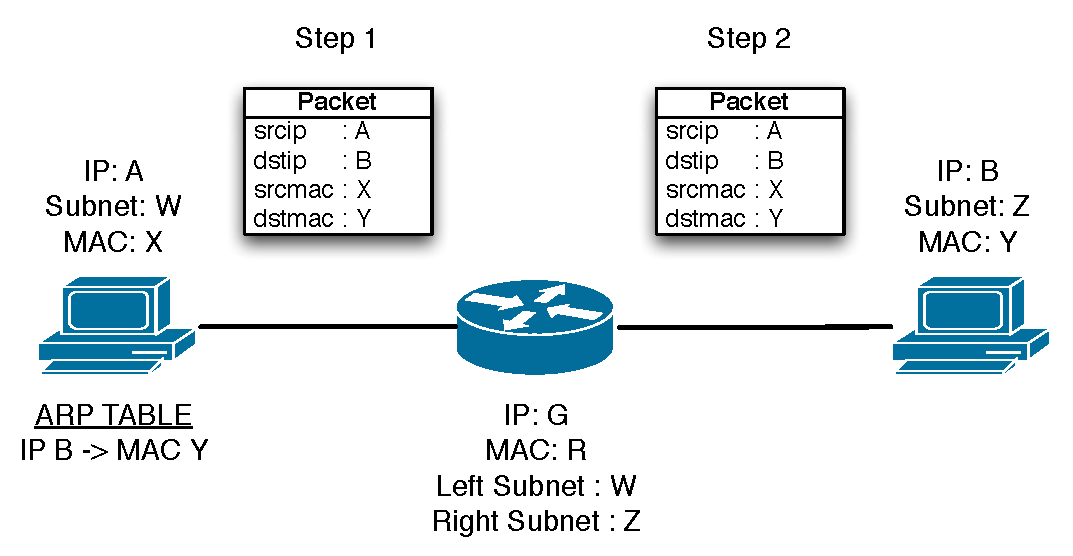
\includegraphics[width=\textwidth]{HProuting}}
  \caption{An explanation of routing processes.}
  \label{fig:routing}
\end{figure}

Our goal is to develop a protocol which achieves its routing function without
replacing the Link Layer information, which is mainly how a router behaves
\cite{RFC1812}. The Link Layer information is replaced by a router in order to
be able to direct a packet to its next-hop whilst maintaining the source and
destination IP fields intact. This is easily solved in an OpenFlow
implementation as we can direct packets out of any interface at any moment. The
more crucial problem arises when the packet is arriving at its destination.
Because we will not be able to re-write the MAC address, which is set to the
MAC address of the last-hop router, the destination host will reject the
packet. The workaround here is rather cumbersome, we prepopulate each host ARP
table with the IP to MAC address mappings, and therefore when a host sends
out a packet to any other host it can already set the destination MAC address
to its final value. These two workarounds allow us to design a routing
protocol albeit slightly simplified but the main routing function, of routing
packets through a network via the most efficient path, is still guaranteed.
Figure \ref{fig:normalrouting} depicts the normal behavior of a router and Figure
\ref{fig:HProuting} shown the behavior of routing in our OpenFlow testbed. In
Figure \ref{fig:normalrouting}, a host with IP address A sending traffic to
another host with IP B would first notice that due to its subnet mask that the
destination IP is not on the same local area network (LAN). Therefore, it builds
a packet with source and destination IP A and B respectively and source and
destination MAC address X and R respectively (Step 1).  When the packet arrives
at the router, the router performs an ARP request to determine the MAC address
associated to IP B (Step 2). Once the MAC address is resolved, the router
rewrites in the packet and sends the packet to the destination (Step 3). In
Figure \ref{fig:HProuting}, since the HP Openflow firmware is not able to do any
re-writing (efficiently, at least), we prepopulate the ARP table at every host
for all other hosts. This results in that the packet built at Step 1 already
contains the correct MAC address for the destination IP. Therefore, the router
performs no MAC address lookup and simply forwards the packets to the
destination (Step 2).

%%%SUBFIG ROUTING!!!

\subsection{Network Installation}

\ifigure{TestBed}{0.6}{The testbed as it is implemented at CERN's computing center.}{fig:testbedreal}

The testbed, shown in Figure \ref{fig:testbedreal}, is designed to provide isolated connectivity for OpenFlow experiments while providing hosts and network testers (see
Section \ref{sect:GETB} for experimental evaluation). This is achieved by
deploying connectivity via three networks. First, comes the connection to CERN's
General Purpose Network (GPN), then there is the Control Network (CN) and
finally the OpenFlow network (OF). 

%\begin{figure}
  %\centering
  %\subfloat[The testbed as it is implemented at CERN's computing center.]{\label{fig:testbed}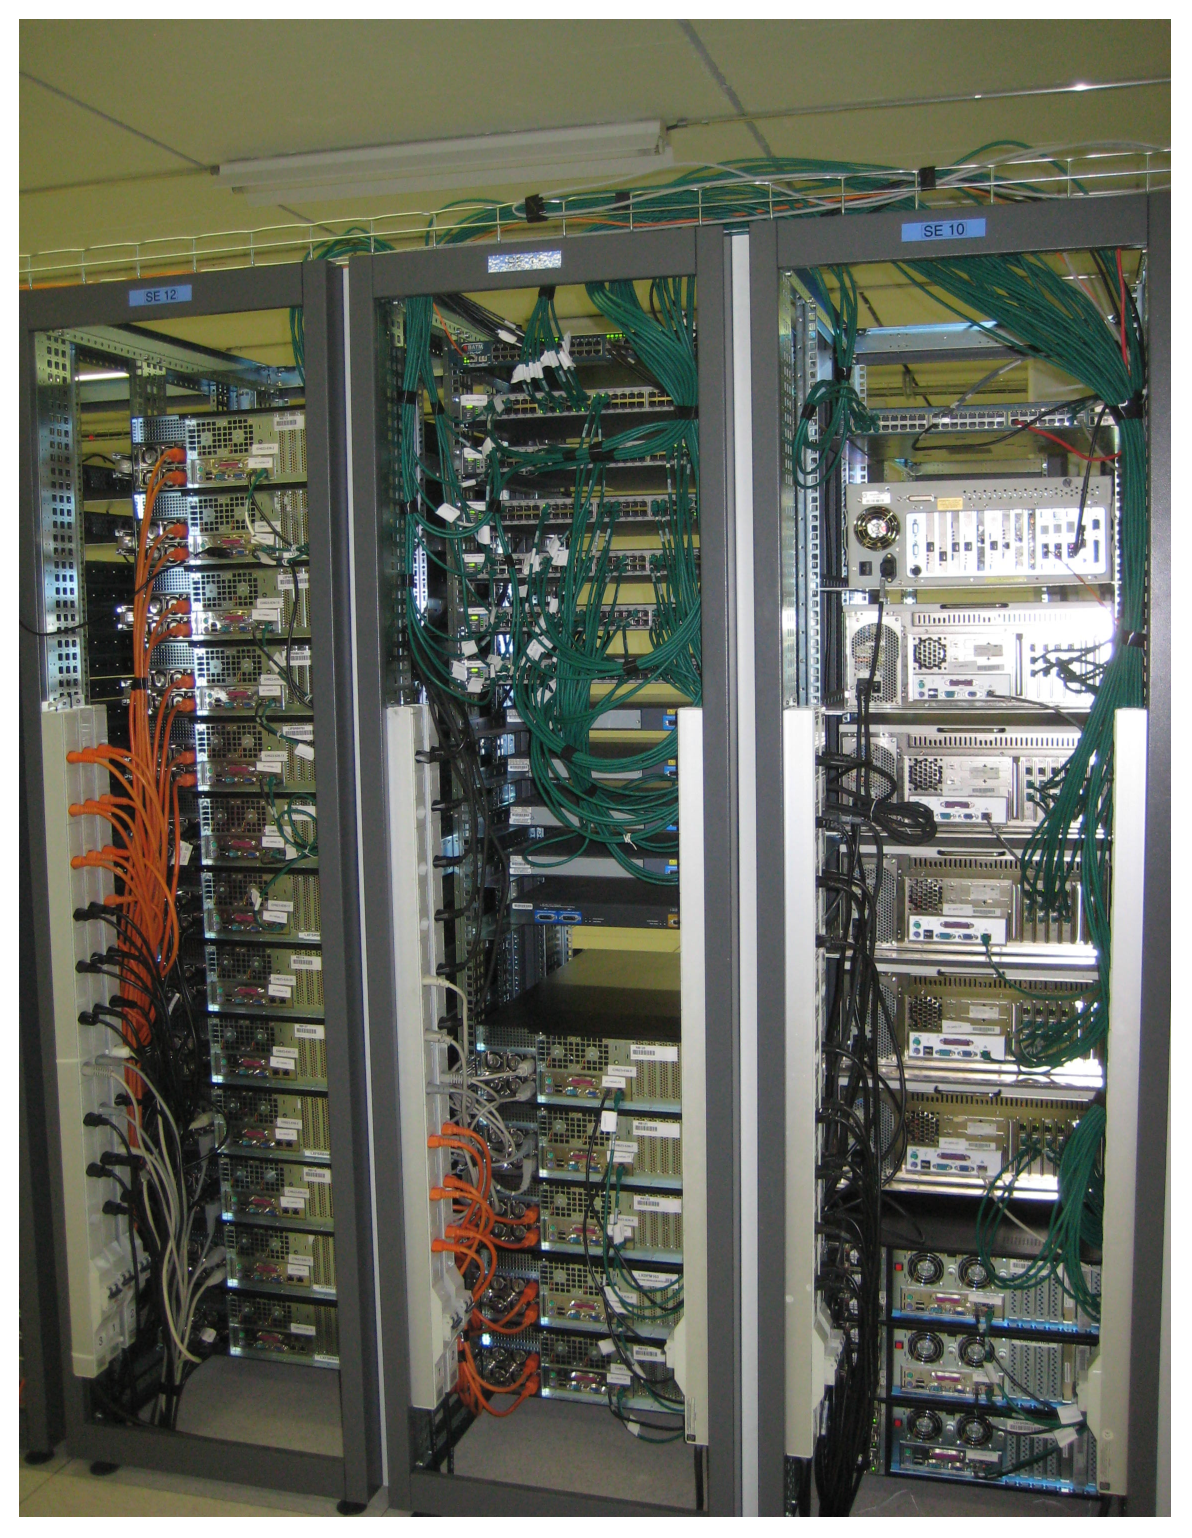
\includegraphics[width=0.5\textwidth]{testbed}}   \\             
 % \subfloat[The connectivity map of the Testbed.]{\label{fig:schema}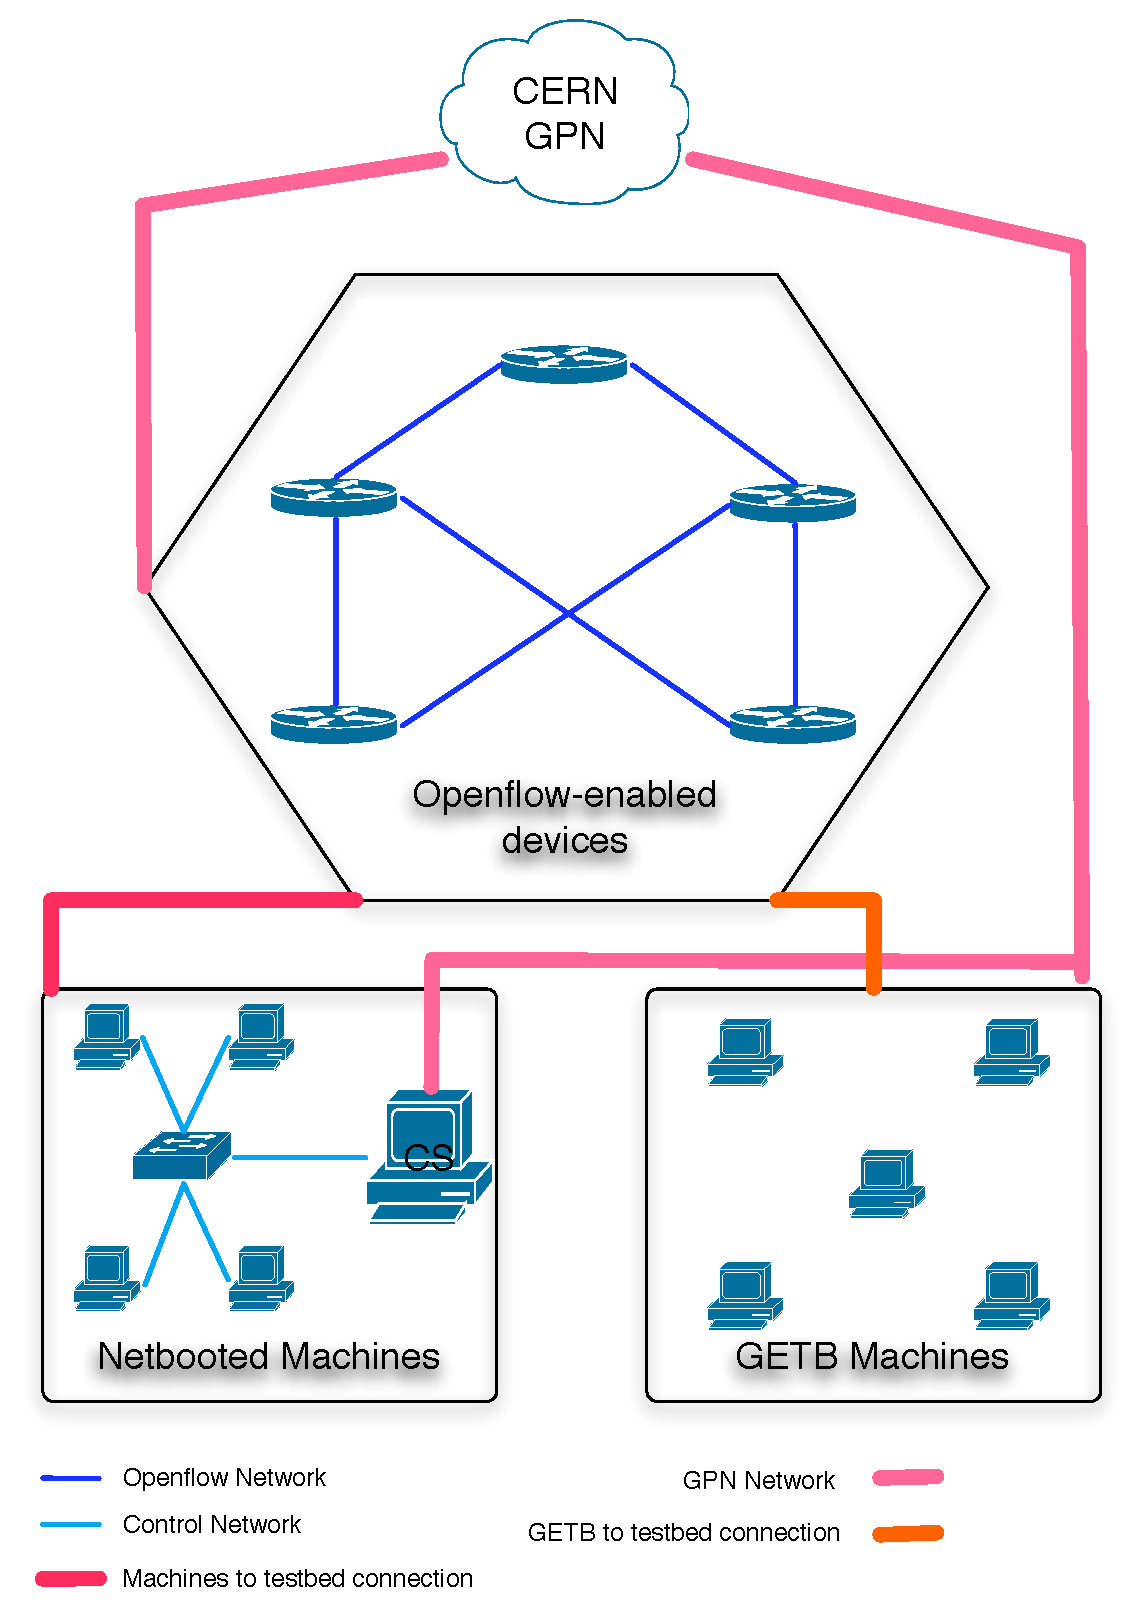
\includegraphics[width=0.7\textwidth]{TestbedSchema}}
 % \caption{The testbed in CERN.}

%\end{figure}



Figure \ref{fig:schema} shows the block connectivity map used with our testbed. The GPN provides connectivity to the world which allows us to install software
on the hosts and update the firmware running on the switch devices. The CN is
the command and control network, which provides the Network FileSystem
(NFS) where the data and systems are stored for the hosts. The GETB Machines (see \ref{sect:GETB} for a complete description) are installed as individual machines each connected to the GPN via its own interface. The OF is the actual connectivity which defines the topology of our test network, as shown in Figure \ref{fig:schema}.

\ifigure{TestbedSchema}{0.5}{The connectivity map of the Testbed.}{fig:schema}

\subsection{Machine deployment}

The hosts are netbooted\footnote{Netbooting consists in booting machines from a
server over the network. These machines can either be diskless or not, but all
the boot information is contained on the network server.} from the Central
Server (CS). Each is configured to obtain an IP address at boot time via the
Dynamic Host Configuration Protocol (DHCP). DHCP provides the hosts
with extra information such as the gateway address, and the netbooting
server. The host downloads a bootloader from the netbooting server and boots as
if it had the bootloader locally. The bootloader instructs the host to mount an
NFS volume where all the boot and data for the host to run is contained. For
more information on netbooting, the reader is referred to \cite{Netboot}.

Each host has a dedicated directory on the CS which contains the specific
configuration of that particular host. Therefore, each host behaves as a
diskless machine and pulls its root filesystem from the CS. This approach has
several advantages. First, the configuration of the hosts is simplified as
they can all be done on the CS. Second, deployment of a new machine is accelerated as
we can simply copy another hosts' directory and modify the configuration. Third,
since the directory containing all the applications used by the hosts is shared
by all the hosts, we just need to install application into this directory and
it is directly available on all the hosts.

\section{GETB Network Testers}
\label{sect:GETB}

The Gigabit Ethernet TestBed \cite{GETB} (GETB) is a FPGA-based platform
designed to provide a flexible and fully programmable device testing environment.
The GETBs were designed to deliver full 1Gb/s wire speed full duplex for two ports running concurrently.

Modifications to the FPGA firmware are difficult and time consuming. This is why
the GETB was programmed to offer services. A set of relatively simple
functions were implemented in the FPGA. These were then used as building blocks
for more complex behavior – the hardware functions were accessible to the user
through the GETB control software (GETB/CS).
   
The aim of the GETB/CS was to provide a common control infrastructure for all
the GETB-derived projects. We needed a system flexible enough to allow complete
customization for the different applications. We also wanted to be able to
easily automate the actions of the GETB cards. This requirement practically
excluded the development of a Graphical User Interface specifically for the
GETB (which we thought would limit the functionality and would be difficult
to maintain and further improve). Finally, our decision was to build almost all
the GETB control system using the Python scripting language \cite{Python}.

The GETB/CS is divided into two main components: the server component – which
runs on the computers hosting GETB cards; and the client component running on
any other machine which needs to access the resources of the servers. Each
machine which contains GETB cards runs the server component. Then, the client
is run on a different machine and controls the operation of the GETB cards.

The GETB cards enable you to generate traffic at various rates and in a
controlled fashion. Therefore, we are able to devise test scenarios with a relatively
large port density as we can connect up to 32 GETB simultaneously.


\section{Experimental Technique}

Now that we have described our experimental testbed setup and and the
associated network tester, we are going to briefly define the methods used to
test our protocols. 

\subsection{Parasite Traffic}

In this test, we measure the capacity of the network device to forward traffic
in the presence of interfering traffic. This test will indicate the capacity of
the router to avoid areas with pre-existing congestion.

\subsection{Fully Meshed Traffic}

Fully meshed traffic, in which traffic is transmitted from all active
ports to all other active ports. This will allow us to determine the
drop-rates and throughput.

\subsection{Latency}

In this scenario the idea is to measure the time required to transmit a packet
from one host to another while the network is transporting traffic at different
rates. Doing so will bring out the capability of the routing protocol to route
traffic efficiently and through the current best path.

\section{Summary}

In this section, we have presented the tools which have enabled us to develop our congestion-aware protocols. Moreover, we have introduced the technologies which allow us to deploy our testbed and end nodes. Finally, we have described our tester boards which will generate the traffic we need to test our protocols. The next section will present the results obtained from our test environment.

\chapter{Results \& Discussion}
\label{chap:results}

\ifpdf
    \graphicspath{{7-Results/Chapter7Figs/PDF/}{7-Results/Plots/}}
\else
    \graphicspath{{7-Results/Chapter7Figs/}}
\fi

\begin{flushright}
 \textit{\textquotedblleft Insanity: doing the same thing over and over again \\
 and expecting different results.\textquotedblright}\\
\textit{-- Albert Einstein}
\end{flushright}


In this chapter we will present the most notable results which were obtained
from our real-world testbed implementation. First, we will present a scenario
in which our protocols perform exceptionally well. Then, we show that even in
the extreme worst cases, our protocols still present an improvement over the
legacy protocols. Finally, we show how the latency and packet loss are affected by our
protocols. But before presenting the results we should introduce the topologies
on which the results where generated.

\section{Test Topologies \& Associated Routing Tables}

The Flower, shown in Figure \ref{fig:flower}, is the first topology we present.
It consists of a fully connected square with two networks at either side of this
network. This topology is quite common in campus networks as it provides
redundant paths between the exterior networks (SW1 and SW6 in this case). While
it contains relatively many links it only delivers a maximum of two absolutely
independent paths from any source to any destination. 

\ifigure{Flower}{0.76}{The Flower topology.}{fig:flower}


\begin{table}[h!]
  \begin{center}
    \begin{tabular}{| c | c || c | c | c | c | c | c |}
    \hline
      \multicolumn{2}{|c|}{\multirow{2}{*}{}}  &
\multicolumn{6}{|c|}{Destination} \\
    \cline{3-8}
       \multicolumn{2}{|c|}{} & SW1 & SW2 & SW3 & SW4 & SW5 & SW6 \\
    \hline
    \multirow{6}{*}{\rotatebox{90}{Source}} & SW1 & L & 47 & 48 & [47,48] &
[47,48] & [47,48] \\
    & SW2 & 47 & L & 45 & 43 & 41 & [43, 41] \\
    & SW3 & 48 & 45 & L & 39 & 37 & [37, 39] \\
    & SW4 & [43, 39] & 43 & 39 & L & 46 & 37\\
    & SW5 & [41, 37] & 41 & 37 & 46 & L & 40 \\
    & SW6 & [38, 40] & [38, 40] & [38, 40] & 38 & 40 & LOCAL \\
    \hline
    \end{tabular}
  \end{center}
  \caption{The routing table associated to the Flower topology.}
\label{tab:flowerRoute}
\end{table}


The low number of independent paths means that the opportunity for leveraging
the alternative paths is reduced. Therefore, the full-mesh runs should
display similar results regardless of the protocol used. It's associated
routing table is shown in Table \ref{tab:flowerRoute}.

The next topology used is called the Pentagon due to its pentagonal shape. This
topology presents many more alternative paths from a given source to any
destination. This topology is also quite common in campus networks as it
consists of a starpoint centered on SW6, neighboring networks are then
connected to each other to provide redundancy. The routing table is shown in
Table \ref{tab:pentagonRoute}. 



\ifigure{Pentagon}{0.76}{The Pentagon topology.}{fig:Pentagon}


\begin{table}[h!]
  \begin{center}
    \begin{tabular}{| c | c || c | c | c | c | c | c |}
    \hline
      \multicolumn{2}{|c|}{\multirow{2}{*}{}}  &
\multicolumn{6}{|c|}{Destination} \\
    \cline{3-8}
       \multicolumn{2}{|c|}{} & SW1 & SW2 & SW3 & SW4 & SW5 & SW6 \\
    \hline
    \multirow{6}{*}{\rotatebox{90}{Source}} & SW1 & L & 26 & 27 & [26,25] &
[27,25] & 25 \\
    & SW2 & 26 & L & [26, 27] & 28 & [27, 28, 26] & 27 \\
    & SW3 & 27 & [27, 29] & L & [29, 30, 27] & 30 & 29 \\
    & SW4 & [28, 31] & 28 & [31, 32, 28] & L & 32 & 31\\
    & SW5 & [30, 33] & [32, 33] & 30 & 32 & L & 33 \\
    & SW6 & 25 & 27 & 29 & 31 & 33 & L  \\
    \hline
    \end{tabular}
  \end{center}
  \caption{The routing table associated to the Pentagon topology.}
\label{tab:pentagonRoute}
\end{table}

It should be also noted that the entries in the routing tables are sorted by
distance to the destination. Therefore, the leftmost entry is the shortest to
the destination. Moreover, each link in the experimental network runs at 1Gb/s.

Each of these topologies are connected to the GETB machines. There are 32 connections to the GETB machines and there are six switches, therefore we have chosen to drop two GETBs and have five connections per switch. The communication path for the GETBs is determined programmatically and depending on the scenario employed.

\section{Parasite Traffic}

In this section we will present results for both topologies when faced with parasite traffic. The idea of these tests is  to run a UDP stream (ie. The parasitic traffic) on a segment over the entire shortest path between two nodes. Then, two TCP flows are sent between the two same nodes. We then compare our results with Shortest Path (SP) only routing and the Hash-Threshold variant of ECMP (HTE).

\subsection{Parasite Traffic on the Flower Topology}

In this setup, parasitic UDP traffic is sent from SW2 to SW6 via SW4. Then, two TCP flows are sent from SW1 to SW6 and the behavior of each protocol is observed.

\subsubsection{Shortest Path versus MultiRoute}

\ifigure{Flower/PDF/MRvsSP}{.38}{Shortest Path versus MultiRoute in the presence of Parasitic traffic.}{fig:MRvsSPFlower}

Figure \ref{fig:MRvsSPFlower} shows MultiRoute's behavior in the presence of parasitic input load. We can see that as the parasitic traffic rate increases, one of the flows gradually ramps down while the other is running at line rate. This situation indicates that during these runs MultiRoute did not mark the link running the parasitic traffic as congested, because the associated transfer function was not sensitive enough. Once this link is marked, the two flows share links along the path to the destination, and this causes TCP's congestion control to rate limit the traffic and therefore we observe that both flows share the bandwidth between themselves. Figure \ref{fig:MRvsSPFlower} also presents the results when running a shortest path only protocol. As expected, the two TCP streams share the available bandwidth between themselves and as the parasitic traffic rate increases, we observe the throughput for both flows being significantly affected. 


\subsubsection{Shortest Path versus StepRoute}

\ifigure{Flower/PDF/SRvsSP}{.38}{Shortest Path versus StepRoute in the presence of Parasitic traffic.}{fig:SRvsSPFlower}

When running StepRoute, classes of congestion are used, and therefore as the parasitic load increases it is classified into different congestions levels. As a TCP flow consumes the entire bandwidth available, StepRoute directly classifies the paths used by the first TCP stream into the highest congestion class. Therefore the paths used by the TCP stream are considered to be a worse option than the ones carrying the parasitic load as the parasitic traffic classifies into lower congestion levels. Thus, on Figure \ref{fig:SRvsSPFlower} we see that one TCP flow runs unhindered at line rate while the other shares with the parasitic traffic until the parasitic traffic is classified into the highest congestion level, at which point the TCP flows share the same paths and therefore share the available bandwidth,

The issue with this behavior is that UDP does not cooperate with TCP (or with anyone for that matter) as it does not implement the congestion control algorithms that TCP does, which means that the UDP traffic will continue to to use all the bandwidth it needs and leaves the remainder for the effective TCP traffic. Therefore, on Figure \ref{fig:SRvsSPFlower} we see that the second TCP flow is affected significantly by the parasitic traffic but it is never worse than the shortest path. 

%SR uses levels of congestion therefore parasite is deemed less harmful than tcp which uses up all bandwidth. problem is udp does not play nice.

\subsubsection{Shortest Path versus PathRoute}

\ifigure{Flower/PDF/PRvsSP}{.38}{Shortest Path versus PathRoute in the presence of Parasitic traffic.}{fig:PRvsSPFlower}

PathRoute uses the same congestion marking scheme as MultiRoute. Therefore, the first part of Figure \ref{fig:PRvsSPFlower} behaves similarly to MultiRoute where one flow goes along the alternative path and the other flow shares the traffic with the parasitic traffic. But as the parasitic traffic increases in intensity, the segments which it uses are eventually marked as congested, but as the first segment of the path SW1 to SW6 is not congested at all, the first flow uses it  and then reroutes via SW5, this causes the segment SW1 to SW2  to be congested. When the second flow arrives it avoids the congested area totally and therefore takes the option containing less congested segments, this causes the second flow to share bandwidth with the parasitic traffic. This explains the seemingly exchange in roles between the two TCP flows. Eventually, all the segments used by the parasitic traffic are marked as congested causing both TCP flows to avoid the congested area and share bandwidth.

\subsubsection{Hash-Threshold versus MultiRoute}

%\ifigure{Flower/PDF/MRvsHTE}{.38}{A comparison of the predictability of MultiRoute versus Hash Threshold}{fig:MRvsHTEFlower}

\begin{figure}[!htbp]
  \centering
  \subfloat[MultiRoute's throughput variation]{\label{fig:MRvsHTEa}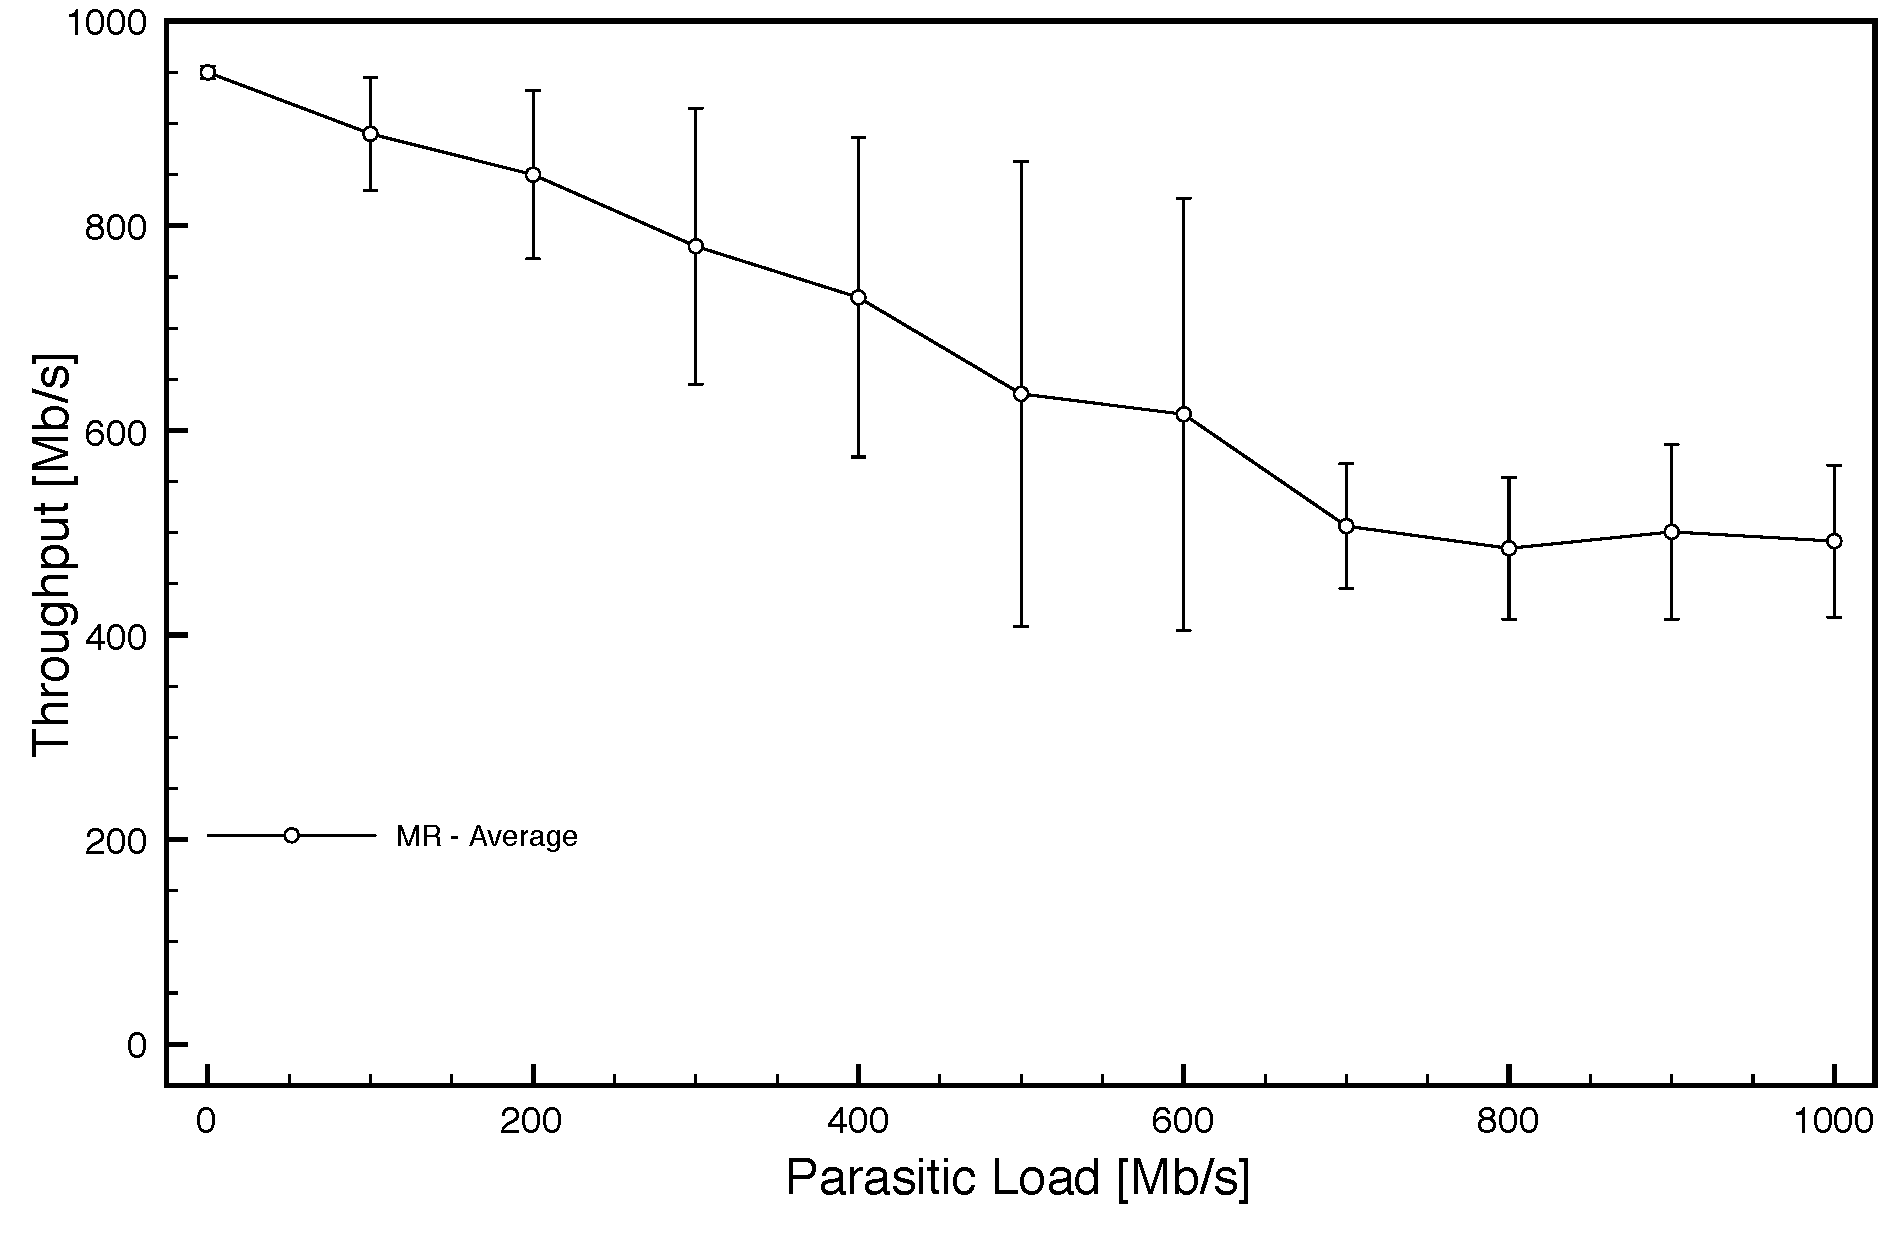
\includegraphics[scale=0.38]{Flower/PDF/MRVar}} 
  
  \subfloat[Hash Threshold's throughput variation]{\label{fig:MRvsHTEb}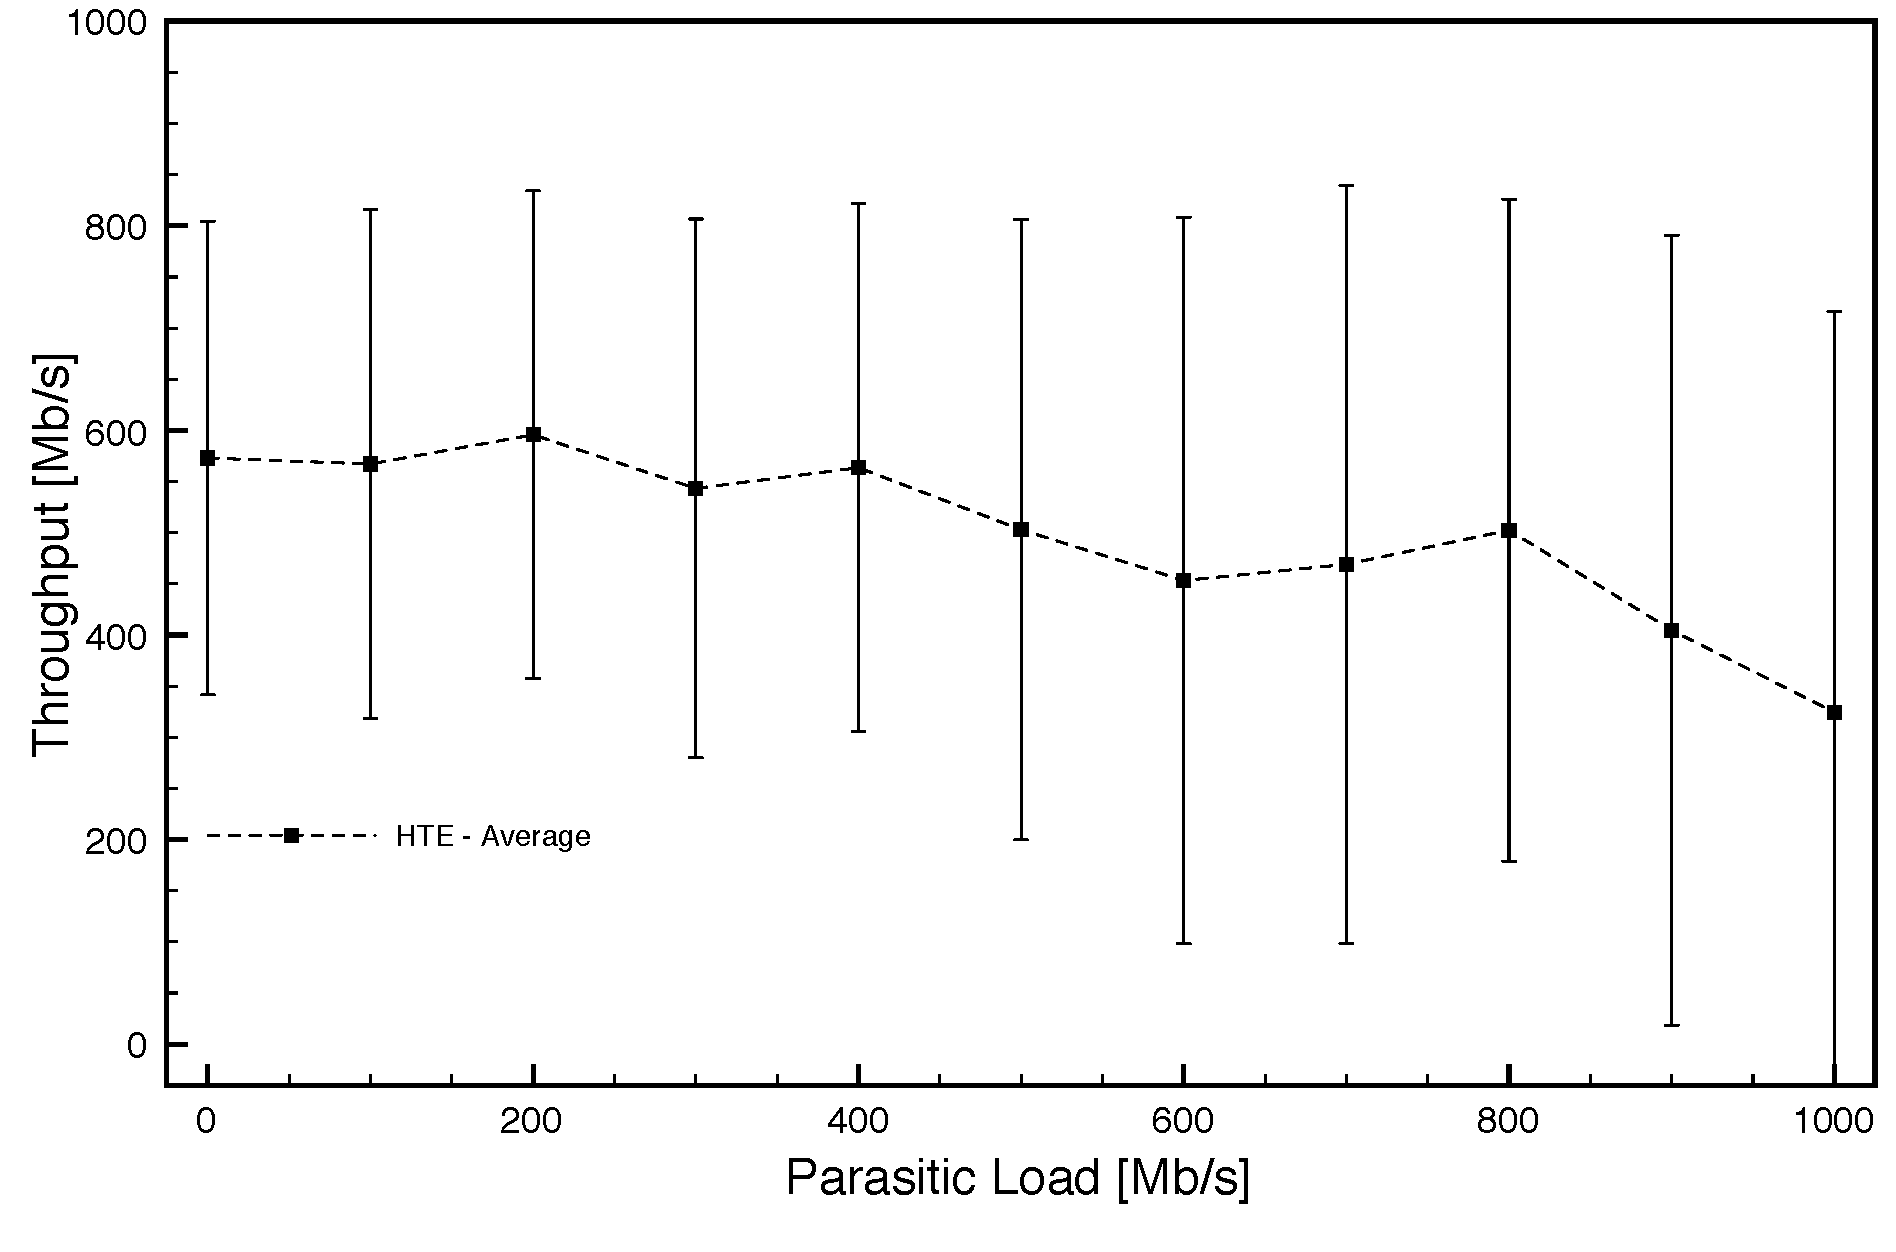
\includegraphics[scale=0.38]{Flower/PDF/HTEVar}}
  \caption{A comparison of the predictability of MultiRoute versus Hash Threshold}
  \label{fig:MRvsHTEFlower}
\end{figure}

Figure \ref{fig:MRvsHTEFlower} shows the average throughput with error bars which represent the variation in throughput observed when running our tests for MultiRoute (Figure \ref{fig:MRvsHTEa}) and HTE (Figure \ref{fig:MRvsHTEb}) . These measurements where done while varying the parasitic traffic rate. Considering only the result for HTE, we observe a large variation of minimum and maximum values. This is explained by the fact that HTE does not consider congestion statistics, and therefore flows may in one case share links and not in others. This phenomenon is especially apparent when the parasitic traffic is high, in some cases all flows will share the same path as the parasitic traffic, causing quasi null throughput for these flows, and in others one flow will be alone on an uncongested path resulting in line rate throughput. These results show that in such situations, HTE throughput can become difficult or nearly impossible to predict accurately. Consider now the results for MultiRoute, the variance between the maximum and minimum values is significantly smaller than in the case of HTE, especially when the parasitic traffic is high. As the parasitic traffic increases in intensity, MultiRoute will route all TCP flows onto the same path causing, like in Figure \ref{fig:MRvsSPFlower}, to share the available bandwidth while avoiding the path used by the parasitic traffic.These results show that we can predict with a significantly higher degree of confidence the expected throughput of MultiRoute in the presence of other traffic flows. It is also interesting to notice than in average MultiRoute performs better than HTE.

\subsection{Parasite Traffic on the Pentagon}

In this setup, parasitic UDP traffic is sent from SW2 to SW5 via SW6. Then, two TCP flows are sent along that same path. 

\subsubsection{Shortest Path versus MultiRoute}

In this situation, there is more than one alternative path to the destination. Therefore, it is expected that all the congestion aware protocols will eventually use all the available paths and therefore avoid the parasitic traffic altogether. Indeed, as we can see in Figure \ref{fig:MRvsSPPentagon}, one TCP flow shares the shortest path to the destination with the parasitic traffic but then switches to an alternative path when the shortest path is marked as congested.  

\ifigure{Pentagon/PDF/MRvsSP}{.38}{Shortest Path versus MultiRoute in the presence of Parasitic Traffic.}{fig:MRvsSPPentagon}

\subsubsection{Shortest Path versus StepRoute}

When running this test with StepRoute, we observe the same behavior except that both TCP flows quickly run at line rate as can be seen in Figure \ref{fig:SRvsSPPentagon}. This can easily be explained by the fact that StepRoute uses congestion classes and not a single bit only. Therefore, as StepRoute quickly marks the link used by the parasitic traffic as lightly congested, it directly uses the alternative path to the destination. We can therefore say that StepRoute is quite sensitive to the congestion status of the various paths. 

\ifigure{Pentagon/PDF/SRvsSP}{.38}{Shortest Path versus StepRoute in the presence of Parasitic Traffic.}{fig:SRvsSPPentagon}

\subsubsection{Shortest Path versus PathRoute}

Figure \ref{fig:PRvsSPPentagon} shows the same test when running PathRoute. Since MultiRoute and PathRoute use the same mechanism to detect and represent congestion we observe a similar result to the one presented in Figure \ref{fig:MRvsSPPentagon} with MultiRoute. But the performance of PathRoute is significantly lower than  MultiRoute or StepRoute. This can be explained due to the longer feedback loop which is introduced by PathRoute's complexity (ie. the knowledge of congestion for a source to any destination). The long feedback loop causes PathRoute to take decisions which are out of sync with the current network status.

\ifigure{Pentagon/PDF/PRvsSP}{.38}{Shortest Path versus PathRoute in the presence of Parasitic Traffic.}{fig:PRvsSPPentagon}

\section{Fully-Meshed Traffic}

Fully-Meshed traffic is the worst possible situation for our protocols as they represent conditions where congestion is equal and omnipresent throughout the network. These tests were performed using the GETB boards. Four end nodes were connected to each switch then each end node sends traffic to each other end node at varying loads from 1\% to 25\% (as this sums up to 100\% for each switch) and the behavior of each protocol is observed. 

For both topologies, one might expect to see a linear throughput until some asymptotic limit, but this is not what was observed in either case. This can be explained by the fact that effective throughput is essentially a function of a switch's packet drop probability. The higher this probability is, the lower the throughput will be. Therefore, when traffic is run through one switch we observe linear increase in throughput as the load increases, because the drop probability is a linear function of the load. Unfortunately this is not the case when there are multiple switches connected to each other. Indeed, while the packet drop probability is still a function of the load, it is now also conditional on the packet drop probability of the previous switch. This conditional probability manifests itself in the following plots as variations (or ``kinks'') in the measured throughput curves.

An attempt was made at modeling this conditional probability using Bayesian Networks \cite{BayesNetwork}, but the model turned out to be vastly too complex and resulted in a combinatorial explosion for the expression of this probability.

%\newpage

\subsection{Fully-Meshed Traffic on the Flower}

\ifigure{Flower/PDF/FullMesh}{.35}{Fully-Meshed Traffic running on the Flower.}{fig:FMFlower}

As is shown in Figure \ref{fig:FMFlower}, all the protocols seem to perform similarly. We can explain this by the fact that all the paths are congested and therefore our congestion aware protocols quickly default to the shortest path. That said, there is a slight (albeit marginal) increase in performance for our protocols. This increase in performance can be better observed when the tests are run successively in order to eliminate the effect of the variations in the throughput as shown in Figure \ref{fig:FMFlowerProbable}. We observe that even though the throughput for both protocols is similar, we clearly notice that as the load increases the difference in the throughput between the shortest path protocol and the congestion-aware increases in average. Actually, there is about a 2GB difference on average, this equates to roughly 66MB every second which means that our protocols have added $\frac{2}{3}$ of a Gigabit link over a shortest path protocol. We believe that this a significant achievement in a Fully-Meshed environment.

\ifigure{Flower/PDF/ProbableLosses}{.38}{Successive Fully-Meshed Traffic running on the Flower.}{fig:FMFlowerProbable}

\subsection{Fully-Meshed Traffic on the Pentagon}

In a topology which offers more alternative paths, we clearly see that our protocols consistently outperform legacy protocols. It is particularly interesting to observe that the Hash Threshold variant of ECMP performs least well. We can explain this by the  manner in which HTE selects its next-hop (based on the source and destination MAC addresses), source-destination pairs will always use the same path regardless of the load they impose on the network and therefore not only does HTE overload those paths it also uses longer congested paths to the destination which significantly decreases its performance.


\ifigure{Pentagon/PDF/FullMesh}{.38}{Fully-Meshed Traffic running on the Pentagon.}{fig:FMPentagon}

\section{Latency \& Packet Loss Tests}

These final results were also obtained using the GETB boards. Full-Mesh traffic was run on each topology, then a stream of probe traffic was sent between two nodes on the network. The time of arrival of the probe traffic as measured and the number of packets lost was counted.

Before explaining the results in this section, we should comment the pseudo step function that is observed in both latency plots below. The linear part of the curve can be seen as the buffers at a router filling, once full we see a significant increase in latency as the switch requires more time to let a packet through its full buffers. From the theory we would expect a linear increase as the router buffers fill up followed by a flat line when all the buffers are full. Unfortunately, this is where our theory and practice differ as it is mathematically complex to construct a queuing model which can tolerate losses. If we consider a single router situation we would observe a linear increase followed by a flatline as the buffers start to drop packets. But now, as we have several routers in a row, we observe a step function which is explained by the fact that a router who is dropping packets has an influence on the loss probability of the next router in the chain who now has a lower loss rate due to a lighter input. Hence, we observe a step function as the routers in the chain have differing rates of buffer saturation.

\subsection{Latency \& Packet loss on the Flower}

\ifigure{Flower/PDF/Latency}{.3}{Latency plots for protocols running on the Flower.}{fig:FlowerLatency}

\ifigure{Flower/PDF/PacketLoss}{.3}{Packet Loss for protocols running on the Flower.}{fig:FlowerPacketLoss}

Figures \ref{fig:FlowerLatency} and \ref{fig:FlowerPacketLoss} show the latency and packet loss experienced by the different protocols respectively. In the case of latency we can see that our protocols present paths which provide less latency, which is to be expected because in this topology we have alternative paths of identical lengths and therefore our latency should either be equal to the shortest path or less. For packet loss, we see that both MultiRoute and StepRoute perform better than the other protocols, this is consistent with our previous results (see Figure \ref{fig:FMFlower}) as they present increased performance in terms of throughput. On the other hand PathRoute performs less well, but again this is consistent as PathRoute does not perform well in terms of throughput during a full-mesh.

\subsection{Latency \& Packet loss on the Pentagon}

\ifigure{Pentagon/PDF/Latency}{.3}{Latency plots for protocols running on the Pentagon.}{fig:PentagonLatency}

\ifigure{Pentagon/PDF/PacketLoss}{.3}{Packet Loss for protocols running on the Pentagon.}{fig:PentagonPacketLoss}

In this case, it is interesting to see that protocols, namely MultiRoute and StepRoute, present a higher latency as shown in Figure \ref{fig:PentagonLatency}. We can explain this by simply noticing that the alternative paths for this topology are longer that the shortest path and therefore require a higher transit time. Figure \ref{fig:PentagonPacketLoss} confirms this observation as the packet loss presented by StepRoute and MultiRoute is lower than the Shortest Path protocol, which means that an alternative path must have been used else the packet loss would have been similar to the shortest path.

\section{Summary}

As these results have shown, our congestion-aware protocols have outperformed legacy protocols. Both, in worst case situations (Full-Mesh) and rather advantageous positions (Parasitic Traffic). Nevertheless, deployment of such protocols requires a rigorous study of the type of services which will de offered by the network. For example, if a network is supposed to carry mainly Voice-over-IP traffic then the network engineer should make sure to provide paths of identical lengths to all destinations in an effort to keep the traffic latencies constant. 

Naively, one would expect that a protocol which has quasi network wide knowledge, such as PathRoute, would deliver optimal results. Unfortunately this is not the case, from the results presented in this chapter we clearly observe that PathRoute performs significantly worse than its peers (MultiRoute and StepRoute). This phenomenon is exacerbated when we consider fullmesh situations. The reason for this lack in performance can be found in control theory's standard problem, ie. the duration on the feedback loop. While all the congestion-aware routing protocols presented in this thesis suffer from a delay between observing congestion and adapting the network state to reflect this change, the impact on PathRoute is more significant that on its peers. Indeed, any update in any area of the network may, in the worst case, trigger updates at all the routers in the network and therefore cause some routers to have opposing network views thereby causing poor routing decisions to be taken.

%Another, rather disappointing, observation is that  PathRoute did not perform as well as we would have liked (or indeed expected). The explanation lies within that fact that PathRoute requires a relatively large amount of signaling and that it assumes that updates from routers which lie on a path  from a source to a destination are synchronous. This assumption does not hold in PathRoute current implementation as each transfer function is independent of one another and therefore segments of a path may report different congestion states and thus cause source routers to make incorrect routing decisions. A rather simple solution to this would be add an extra layer of signaling for PathRoute, but this could prove to be expensive and may impact the reactivity of the protocol.
\def\baselinestretch{1}
\chapter{Conclusions \& Future Work} 
\ifpdf
    \graphicspath{{8-Conclusions/ConclusionsFigs/PNG/}{8-Conclusions/ConclusionsFigs/PDF/}{8-Conclusions/ConclusionsFigs/}}
\else
    \graphicspath{{8-Conclusions/ConclusionsFigs/EPS/}{8-Conclusions/ConclusionsFigs/}}
\fi
\begin{flushright}
 \textit{\textquotedblleft Finally, in conclusion, let me say just
this. \textquotedblright}\\
\textit{-- Peter Sellers}
\end{flushright}

\section{Achievements}

The objective of this thesis was to revisit the concept of congestion-aware routing. This idea was introduced in the early days of the ARPANET but quickly abandoned due to out of order delivery of packets which caused the effective throughput of the network to be catastrophic. To achieve this goal, we have divided the problem into three sub-problems, namely:

\begin{enumerate}
\item Path Construction -  The multiple path discovery process relies on the existence of a shortest path between source and destination points. After establishing the shortest path cost (the reference cost), each alternate path is computed whose cost is within a reasonable delta of the reference cost. 
\item Network Monitoring - The statistics are polled locally by the router and sent to neighboring routers, this process is performed in-band and not by an external monitoring process. Then, depending on the transfer function used, a representation of the congestion is derived.
\item Topology Representation - Each router maintains its own routing vector, consisting of congestion representation of its paths to different networks. Routing vectors are then exchanged with neighboring routers using the Monitoring protocol .
\end{enumerate}

Using this approach we have been able to build three different congestion-aware protocols which contrast with previous multipath protocols in several aspects. First, they treat alternative paths as another possibility rather than a route to take in case of failure. Second, they do not require full knowledge of the network topology as they obtain the congestion status of their direct neighbors only. Finally, they avoid out-of-order packet distribution by using flows as a basis for routing rather than packets. This coupled with the fact that routing decisions are immutable completely side-steps the problem of out-of-order packets. On the other hand, this raised the following question: \textit{Can a protocol with such restrictions still provide a benefit in term of performance?} We believe that this thesis shows that the answer to this question is \textbf{Yes}!

Another aspect of this thesis was the implementation a real world testbed in which our congestion-aware protocols were deployed. The design, construction and evaluation of this testbed was carefully studied. First, it was designed so that it could easily be extended, for example adding an end node to the test bed is as easy as entering a few configuration lines in the file server and then booting the desired end node. This end node would then have all the functionality previously existing nodes have. Second, the testbed was constructed in such a was that it would be simple to interconnect and physically simple to extend. Finally, by designing and constructing the system with the knowledge that the system would have to be tested, it was simple to provide connectivity to the test machines and the traffic generators. 

\section{Summary of Results}

Based on the results presented in Chapter \ref{chap:results} we believe that we can say that our congestion aware protocols provide an significant increase in performance when compared to legacy protocols. This results have been tested on two representative topologies.

Our protocols perform best when asked to route around a congested area. We show that is some cases our protocols provide line rate performance when shortest path or Equal Cost MultiPath (ECMP) provide close to zero throughput. We also show that even though our protocols are congestion-aware, they provide a predicable throughput where ECMP could not. 

We have also shown that in the face of fierce adversity, ie. Full-Mesh traffic, our protocols provide an increased level of performance. This worst case scenario demonstrates that these protocols can be expected to deliver increased performance on non-traffic engineered networks.

While we show that our protocols present increased performance, a network engineer deploying such protocols should study the requirements of the network he is implementing. We believe the questions that need to be answered are: 

\begin{enumerate}
\item Does the expected traffic tolerate loss?  
\item Does the expected traffic tolerate delay?
\item Does the expected traffic consist of short or long lived flows? 
\item Is the traffic on this network expected to be traced?
\end{enumerate}

The answers to these questions will determine which protocol to use and/or the type of topology to deploy (either equal cost lengths or variable alternative path lengths).

\section{Future Work}

As with any thesis, many lines of research remain. We shall state a few here in the form of open ended questions:

\begin{itemize}
\item How does one trace traffic through a multipath network? Is debugging even possible?
\item What are the effects of using other metrics as a basis for congestion detection?
\item Do our congestion-aware routing protocols scale to networks with hundreds of routers?
\item How can the feedback loop required for congestion-aware routing protocols be made as small as possible?
\item Will it ever be possible to mathematically model multipath networks accurately?
\end{itemize}

%What is the strongest and most important statement that you can make from your
%observations? 
%
%If you met the reader at a meeting six months from now, what do you want them to
%remember about your paper? 
%
%Refer back to problem posed, and describe the conclusions that you reached from
%carrying out this investigation, summarize new observations, new
%interpretations, and new insights that have resulted from the present work.
%
%Include the broader implications of your results. 
%
%Do not repeat word for word the abstract, introduction or discussion.

%%% ----------------------------------------------------------------------

% ------------------------------------------------------------------------

%%% Local Variables: 
%%% mode: latex
%%% TeX-master: "../thesis"
%%% End: 


%% Configuration of the header strings for the Appendices
\renewcommand{\chaptermark}[1]{%
  \markboth{\MakeUppercase{\appendixname\ \thechapter}}%
  {\MakeUppercase{#1}}
}
\fancyhead[RE,LO]{}


\appendix
\chapter{Collection of derivations}
\ifpdf
  \graphicspath{{9-Appendix1/}}
\else
  \graphicspath{{9-Appendix1/}}
\fi

\label{appdx:A}

\section{Disruptions in the Hash Threshold variant of ECMP}
\label{sect:HTE} 

TCP protocols perform superbly in situation where the path they flow does not change during the connection. Disruptions is the measure of how many flows will be affected by a path change. Consider now a hash based next hop selection, if our hash function is uniform then each next hop has an equivalent probability to be selected. Therefore, we can say that the hash-space is equally distributed between next-hops (or regions) as shown in Figure \ref{fig:HashSpace}

\ifigure{HashSpace}{0.7}{Before and After the deletion of the third next hop possibility.}{fig:HashSpace}

We can formalize this by considering the removal of region $K$ in the presence of $N$ regions. This causes the remaining $N-1$ regions to fill the $\frac{1}{N}$ space left by the removal of region K. Therefore each remaining region grows by $\frac{1}{N(N-1)}$. But now, this means that every non-end region has to be moved to accommodate for its now grown neighbor. So the first regions grows and causes the second region to shift towards towards region K by $\frac{1}{N(N-1)}$, and in turn the third region is caused to move by $\frac{2}{N(N-1)}$ and so on until both ends meet at the borders of $K$. These moves causes $\frac{i}{N(N-1)}$ flows in region $i+1$ to to be taken over by region $i$. Therefore, we have the following equations:

 \begin{align}
 disruptions &= \displaystyle\sum\limits_{i=1} ^{K-1}\frac{i}{N(N-1)} +  \displaystyle\sum\limits_{i=K+1} ^{N}\frac{i-K}{N(N-1)}\\
 &= \frac{1}{N(N-1)} \left(  \displaystyle\sum\limits_{i=1} ^{K-1}i + \displaystyle\sum\limits_{i=K+1} ^{N}i-K\right)\\
 &= \frac{(K-1)(K) + (N-K)(N-K+1)}{2N(N-1)}
 \label{eq:disrupt}
\end{align}

Equation \ref{eq:disrupt} formalizes the number of flows which would be disrupted if a link on a path to a next-hop fails. 


\section{Backpressure messages given in AMP}
\label{sect:AMPCALC}

A backpressure message in AMP is given by two factors; consider the link $\overline{XY}$:

\begin{enumerate}
\item The load on the links directly connected to $X$; and
\item The contribution of the traffic routed at $X$ on the links from $Y$ to $Z$ ($\overline{YZ}$).
\end{enumerate}

The first point is immediate as the router can directly measure the congestion on their direct links, this is given by $\rho$. The remaining value describes the messages sent from the neighboring routers called $B_{Z\rightarrow Y}$ which is itself computed based on the two factors described above. Therefore, we can simply note BMs as $B_{Z\rightarrow Y}$, formally $BM(Y,X) = B_{Y\rightarrow X}$. $BM(Y,X)$ is the backpressure message sent from node $Y$ to node $X$. We can now define $ B_{Y\rightarrow X}$ as a function of the directly measurable congestion values and the $B_{Z_{i} \rightarrow Y}$, therefore we have:

 \begin{align}
B_{Y\rightarrow X} = f(\rho_{\overline{XY}_i}, B_{Z_{i} \rightarrow Y}), \forall i = 1, \dots, n
 \label{eq:BM1}
\end{align}

As the contributions to congestion from traffic routed at $X$ vary at each neighboring router, since only a fraction of the overall traffic is routed to a particular neighbor, AMP proposes to define these varying contributions as a weighted average where the weight for link $\overline{YZ_{i}}$ corresponds to the ratio of traffic on the link $\overline{YZ_{i}}$ that has arrived from $X$ via $Y$ and the total traffic on the link $\overline{YZ_{i}}$. Therefore, we have:

\begin{align}
B_{Y\rightarrow X} = \displaystyle\sum\limits_{Z_{i} \in \Omega_{Y} \setminus X}\frac{\beta_{ \overline{ YZ_{ i } } } (X) } { \beta_{\overline{YZ_{i}}}} max(\rho_{\overline{XY}_i, B_{Y_{i} \rightarrow X}})
 \label{eq:BM2}
\end{align}

Where $\Omega_{Y}$ is the set of all neighbors of node X,  $\beta_{\overline{YZ_{i}}} (X)$ is the number of bytes sent from node $X$ via $Y$ to $Z_{i}$, and finally $\beta_{\overline{YZ_{i}}}$ denotes the total number of bytes sent from any node $\in  \Omega_{Y} \backslash X$ via $Y$ to $Z_{i}$.
\section{Dependence of Message Length and Interarrival times}
\label{sect:KLEDEP}

Let us derive the joint probability $P(v_n,a_{2n})$ between the message length and the inter-arrival time at some queue. For this consider the tandem network given in Figure \ref{fig:tandem}, and the following quantities:

$v_n = $ message length of the $n^{th}$ message.

$a_{in} = $ the inter-arrival time between the $(n-1)^{th}$ message and the $n^{th}$ at node i.

Now we recall the assumptions of queuing systems with Markovian properties of Section \ref{sect:queues} where both $v_n$ and $a_in$ are described by exponential distributions, given by:

\begin{align}
\label{eq:inter1}
p(a_{1n}) & = \lambda e^{-\lambda a_{1n}}\\
p(v_n) & = \mu e^{-\mu v_n}
\label{eq:msglen}
\end{align}


Due to these facts, Theorem \ref{th:Burke} holds and thereby we have that the inter-departure times at the first node in the tandem are identical to the inter-arrival times at the second node. Therefore we have:

\begin{equation}
p(a_{2n}) = \lambda e^{-\lambda a_{2n}}
\label{eq:inter2}
\end{equation}
 
When the $n^{th}$ message leaves the first node:

\begin{enumerate}
 \item it is separated by a time gap $g_n$ from the $(n-1)^{th}$ message. Or,
 \item transmitted immediately after the $(n-1)^{th}$ message is done transmitting.
\end{enumerate}

It is clear that Case 1. only occurs if the first node emptied out before receiving the $n^{th}$ message, which happens with probability $1-\rho$. The second case occurs when the first node is busy which has probability $\rho$. Where $\rho = \frac{\lambda}{\mu}$ is the utilization factor as defined in Section \ref{sect:queues}. We now have,

\begin{equation}
 p(v_n, a_{2n} = \rho P(v_n,a_{2n}|node~ 1~ busy) + (1-\rho)P(v_n,a_{2n}|node~ 1~ empty)
\label{eq:jointprobtent}
\end{equation}

Trivially, the probability that message $n$ has length $v_n$ and arrives at $a_{2n}$ such that node 1 is busy is equal to the probability that $v_n = a_{2n}$, otherwise the queue would be idle. Thus,
 
\begin{align*}
P(v_n,a_{2n}|node~ 1~ busy) & = P(v_n = a_{2n}) \\
&= \mu e^{-\mu v_n} \mu_0(a_{2n} - v_n) 
\end{align*}

Where $\mu_0$ is the unit impulse function.

Alternatively, the probability that message $n$ has length $v_n$ and arrives at $a_{2n}$ such that node 1 is empty implies that $a_{2n} - v_n \neq 0 = g_n$, obviously otherwise the queue would always be busy, combined with the fact that the message length permits the queue to become empty. Due to the fact that $g_n$ follows the same distribution as $p(a_{2n})$, we therefore have,

\begin{align*}
P(v_n,a_{2n}|node~1~empty) & = P(a_{2n} | v_n,~ node~1~empty)P(v_n|node~1~empty)\\
& = P(g_n = a_{2n} - v_n)P(v_n|node~ 1~ empty) \\
& = P(g_n = a_{2n} - v_n)p(v_n) \\
& = \lambda e^{-\lambda(a_{2n} - v_n)}\mu e^{-\mu v_n}
\end{align*}

And finally the overall expression becomes:

\begin{equation}
 p(v_n, a_{2n} = \mu e^{-\mu v_n} \mu_0(a_{2n} - v_n) + \lambda e^{-\lambda(a_{2n} - v_n)}\mu e^{-\mu v_n}
\label{eq:jointprobfinal}
\end{equation}

By analysis of Equations \ref{eq:jointprobfinal}, \ref{eq:msglen} and \ref{eq:inter2}, we can clearly see that:

\begin{equation*}
 p(v_n, a_{2n}) \neq p(v_n)p(a_{2n})
\end{equation*}

which, by definition independent events, illustrates the deep dependence between the message lengths and the inter-arrival times. 


\section{The Price of Anarchy in Multipath networks with linear cost functions}

\label{sect:linearanarchy}

First let us define more formally the delay of a flow as a function of the links $l$ it traverses as,

\begin{equation}
 C(f) = \displaystyle\sum\limits_{l} c_{l}(f_{l})f_{l}
\label{eq:costflow}
\end{equation}

where,

\begin{itemize}
 \item $c_{l}$ is the cost induced by a flow on the link $l$,
 \item $f_{l}$ is the amount of flow using link $l$.
\end{itemize}

Due to the fact that the model for Selfish routing is a static one, we only consider flows which are in a state of equilibrium. Therefore it is clear that a flow is not in a equilibrium state if it can shift some traffic to another link while reducing the overall delay of the network. Thus, we have the following definition:

\begin{definition}
  A flow $f$ is a \emph{Nash flow} if for all paths $P_{1}, P_{2} \in P$ and amounts $\delta \in ]0,f_{P_{1}}]$ of traffic, we have:
  \begin{center}
   $c_{P_{1}}(f) \leq c_{P_{2}}(\tilde{f})$\\
  \end{center}
   where,
  \begin{center}
  %\begin{equation*}
  \[\tilde{f} = \left\{ 
    \begin{array}{l l}
	f + \delta & \quad \mbox{if $P = P_{1}$}\\
	f - \delta & \quad \mbox{if $P = P_{2}$}\\ 
	f & \quad \mbox{if $P \notin \{P_{1}, P_{2}\}$}\\   
    \end{array} \right. \]
  %\end{equation*}
  \end{center}
  \label{def:nashflow}
\end{definition}

Alongside the definition of a Nash flow, we have the straightforward definition of an optimal flow, which is simply:

\begin{definition}
 A flow $f$ is considered optimal if it is the flow with minimum possible delay. It is then denoted by $f^{*}$.
\end{definition}

As an example, a Nash flow is illustrated by the first situation in Figure \ref{fig:pigou}, whereas an optimal flow is depicted by the second situation.

Finally, we can define the \emph{worst-possible} ratio between the cost of a Nash flow and that of an optimal flow. This ratio is known as the \emph{Price of Anarchy} and is given by the following relation and Equation \ref{eq:costflow}:

\begin{equation}
 \rho = \frac{C(f)}{C(f^{*})}
  \label{eq:anarchy}
\end{equation}

Let us know postulate that optimal and Nash flows are the same things, just with different delay function. In order to establish this we must establish a relationship between optimal and Nash flow as a function of the delay functions.

\begin{definition}
 If $c$ is a differentiable delay function, then the corresponding marginal delay function $c^{*}$ is defined by:
\begin{equation}
 c^{*} = \frac{d}{dx}(x c(x))
\end{equation}
\label{def:marginalfunc}
\end{definition}

By considering definitions \ref{def:nashflow} and \ref{def:marginalfunc}, we can conclude that:

\begin{definition}
 Let G be a network defined by continuously differentiable delay functions and corresponding marginal delay functions $c^{*}$, then a flow $f$ for G is optimal if and only if it is at Nash equilibrium under the marginal delay functions.
\label{def:optinash}
\end{definition}

Now let us consider a network with linear delay functions of the form $ax+b$, therefore by equation \ref{eq:costflow} we have the expression for the delay in such a network:

\begin{equation}
 C(f) = \displaystyle\sum\limits_{l} a_{l}f_{l}^{2} + b_{l}f_{l}
\label{def:lindelay}
\end{equation}

and thus trivially we have that:

\begin{definition}
 Suppose a network has linear delay functions and $f$ is a flow at Nash equilibrium. Then,

\begin{enumerate}
 \item $c_{l}^{*}\left(\frac{f_{l}}{2}\right) = c_{l}(f_{l})$ for any link l;
 \item The flow $\frac{f}{2}$ is optimal for the same network with have the link capacity.
\end{enumerate}
\label{def:linprop}
\end{definition}

The relations in definition \ref{def:linprop} are simply a result of applying Equation \ref{def:lindelay}. 

We now can express the delay caused by an optimal flow as:

\begin{equation}
 C(f^{*}) \geq C\left(\frac{f}{2}\right) + \displaystyle\sum\limits_{l} c_{l}^{*}\left(\frac{f_{l}}{2}\right)\frac{f_{l}}{2}
  \label{eq:costoptimal}
\end{equation}

By definition \ref{def:linprop} and equation \ref{eq:costflow} we have that:

\begin{align}
  \displaystyle\sum\limits_{l} c_{l}^{*}\left(\frac{f_{l}}{2}\right)\frac{f_{l}}{2} &= \frac{1}{2} \displaystyle\sum\limits_{l} c_{l}\left(f_{l}\right)f_{l} \\
  &= \frac{1}{2}C(f)
  \label{eq:righthand}
\end{align}

All we need to solve now is $C\left(\frac{f}{2}\right)$, this is simple if we recall that we are considering linear cost functions and that therefore we can apply Equation \ref{def:lindelay}:

\begin{align}
 C(\frac{f}{2}) &= \displaystyle\sum\limits_{l} \left(\frac{1}{2}a_{l}f_{l} + b_{l}\right)\frac{f_{l}}{2} \\
& \geq \frac{1}{4}\displaystyle\sum\limits_{l} \left(a_{l}f_{l} + b_{l}\right)f_{l}\\
& = \frac{1}{4} C(f)
\label{eq:lefthand}
\end{align}

By introducing equations \ref{eq:lefthand} and \ref{eq:righthand} into Equations \ref{eq:costoptimal}, we obtain:

\begin{equation}
  C(f^{*}) \geq \frac{3}{4} C(f)
  \label{eq:upper}
\end{equation}

Equation \ref{eq:upper} allows us to conclude that the Price of Anarchy for a multipath network with linear delay functions is at most $\frac{4}{3}$. This result can be extended to polynomial delay functions, and we obtain the following Price of Anarchy as a function of the degree of the polynomials:

\begin{equation}
 \rho = \frac{(p+1)\sqrt[p]{p+1}}{(p+1)\sqrt[p]{p+1}-p} \stackrel{p \rightarrow \infty}{=} \frac{p}{ln(p)}
\end{equation}

%needs marginal cost functions and introduction of some lemma from book!

% ------------------------------------------------------------------------

%%% Local Variables: 
%%% mode: latex
%%% TeX-master: "../thesis"
%%% End: 

\chapter{Collection of Pseudocodes}
\label{appdx:B}
\section{Dijkstra's Algorithm Pseudocode}
\label{sect:dijkpseudo}
\singlespacing
\begin{algorithm}
\caption{Dijkstra's Algorithm}
\label{alg:dijk}
 \begin{algorithmic}
  \REQUIRE A network $ R = (V, E, c), \left| V \right| = n, \left| V \right| = m,$ where $ c: E \mapsto \Re_{+}$ is a weighting of arcs on the graph $ G = (V,E) $. A particular vertex $S \in V$ called the source.
  \ENSURE For all vertex $v \in V$, the lengths $D\left(v\right)$ are guaranteed to be minimal.
  \STATE $D\left(S\right) = 0$
  \STATE $D\left(v\right) = \infty, \forall v \neq S \in V$
  \STATE $\forall v \in V, P_{v} = \varnothing$
  \STATE $Q = V$
  \WHILE{$Q \neq \varnothing$}
    \STATE $ u \leftarrow REMOVE-MIN\left(Q\right)$
%    \IF { $ u = \varnothing$ }
%      \STATE Graph disjoint, QUIT
%    \ENDIF
    \FOR { each $v \in Adj\left(u\right)$ }
      \IF { $D\left(v\right) > D\left(u\right) + c\left(u,v\right)$ }
        \STATE $D\left(v\right) \leftarrow D\left(u\right) + c\left(u,v\right)$
        \STATE $P_{v} = v$
      \ENDIF
    \ENDFOR
  \ENDWHILE
 \end{algorithmic}
\end{algorithm}

\newpage

\section{Bellman-Ford's Algorithm Pseudocode}
\label{sect:bellpseudo}

\singlespacing
\begin{algorithm}
\label{alg:bell}
\caption{Bellman-Ford's Algorithm}
 \begin{algorithmic}
  \REQUIRE A network $ R = (V, E, c), \left| V \right| = n, \left| V \right| = m,$ where $ c: E \mapsto \Re$ is a weighting of arcs on the graph $ G = (V,E) $. A particular vertex $S \in V$ called the source.
  \ENSURE For all vertex $v \in V$, the lengths $D\left(v\right)$ are guaranteed to be minimal.
  \FOR {each vertex $u \in V$}
    \STATE $d[u] = \infty$
    \STATE $p[u] = u$
  \ENDFOR
  \STATE $d[s] = 0$
  \FOR {$i = 1$ to $|V|-1$} 
    \FOR {each edge $(u,v) \in E$} 
      \IF {$(w(u,v) + d[u] < d[v])$}
	\STATE $d[v] = w(u,v) + d[u]$
	\STATE $p[v] = u$
      \ENDIF
   \ENDFOR
  \ENDFOR
 \end{algorithmic}
\end{algorithm}

\newpage

\section{MultiRoute Path Construction - Pseudocode and Proof}
\label{appdx:mrpc}

\begin{algorithm}
 \begin{algorithmic}
  \REQUIRE A Network $ R = (V, E, c), \left| V \right| = n, \left| V \right| =
m,$ where $ c: E \mapsto \Re_{+}$ is a weighting of arcs on the graph $ G
= (V,E)$. A particular vertex $S \in V$, and $\varepsilon$ which is the
tolerance to the optimal path length
  \ENSURE For all vertex $v \in V$, the lengths $D\left(v\right)$ of a
alpha-shortest independant paths
  within $\varepsilon$ of the optimal path length ( the
$\varepsilon$-property). From S to v ($D\left(v\right) = \infty$ if there is no
path from s to v in G) along with the immediate predecessor(s) $P_{v}$ of vertex
v in such a path.
  \STATE $D\left(S\right) = 0$
  \STATE $D\left(v\right) = 0, \forall v \neq S \in V$
  \STATE $\forall v \in V, P_{v} = \varnothing$
  \STATE $Q = V$
  \WHILE{$Q \neq \varnothing$}
    \STATE $ u \leftarrow REMOVE-MIN\left(Q\right)$
    \STATE $ K \leftarrow \{k \in Q | \left| D\left(u\right) - D\left(k\right)
\right| \leq \varepsilon \} $
    \IF { $ u = \varnothing$ }
      \STATE Graph disjoint, QUIT
    \ENDIF
    \FOR { each $v \in Adj\left(u\right)$ }
      \IF { $D\left(v\right) > D\left(u\right) + c\left(u,v\right)$ }
        \STATE $D\left(v\right) \leftarrow D\left(u\right) + c\left(u,v\right)$
        \STATE $P_{v} = P_{v} \cup \{v\}$
      \ENDIF
      \IF { $D\left(v\right) > D\left(k\right) + c\left(k,v\right) and
\left|D\left(k\right) +  c\left(k,v\right) - D\left(v\right) \right| \leq
\varepsilon$ }
        \STATE $D\left(v\right) \leftarrow D\left(k\right) + c\left(k,v\right)$
        \STATE $P_{v} = P_{v} \cup \{k\}$
      \ENDIF
    \ENDFOR
  \ENDWHILE
 \end{algorithmic}
\end{algorithm}

\subsection{Proof}

We will now proove the correctness of the MRPC algorithm. This proof is heavily
based on Dijkstra's algorithms own correctness proof and the Optimality
Principle.

\begin{itemize}
\item{\textbf{Proposition - }\\
  The algorithm terminates with with:\\
\begin{center}
 $\forall v \in V, \delta\left(S,v\right) = D\left(v\right) <
\delta\left(S,v\right) + \varepsilon$,\\
\end{center}
where $\delta\left(S,v\right)$ is the shortest path between S and v.}

\item{\textbf{Case I:} 
\begin{center}
$\delta\left(S,v\right) \leq D\left(v\right)$\\ 
\end{center}
  This is given directly by proof of Dijkstra'a algoritm stating that the
shortest distance between $S$ and $v$ is the one recorded at $v$.}

\item{\textbf{Case II:} 

\begin{center}
$D\left(v\right) < \delta\left(S,v\right) + \varepsilon$ \\
\end{center}
  We only consider an arc if:
\begin{center}
  $D\left(v\right) > D\left(u\right) + c\left(u,v\right) and
\left|D\left(u\right) + c\left(u,v\right) - D\left(v\right)\right| \leq
\varepsilon$
\end{center}

We know: $\delta\left(S,v\right) = D\left(u\right) + c\left(u,v\right)$ because
of the optimality principle and Dijkstra's algorithm.

From the equations above we have that:
\begin{center}
 $\left|\delta\left(S,v\right) - D\left(v\right) \right| \leq \varepsilon$
\end{center}

This gives us three possible cases detailed below.

\begin{enumerate}
\item{$\delta\left(S,v\right) - D\left(v\right) = 0 $ \\
  This case is covered by Case I.}
\item{$\delta\left(S,v\right) - D\left(v\right) > 0 $\\
  In this case we obtain that:\\
\begin{center}
 $\delta\left(S,v\right) - \varepsilon \leq D\left(v\right)$\\
\end{center}
Which is not possible, because we know from Dijkstra that
$\delta\left(S,v\right)$ is the shortest path.}

\item {$\delta\left(S,v\right) - D\left(v\right) < 0 $\\
  Here we have:\\
\begin{center}
 $ D\left(v\right) < \delta\left(S,v\right) + \varepsilon$\\
\end{center}}
Which is indeed what we wanted.
 
\end{enumerate}}
\end{itemize}

\newpage
\section{MultiRoute Protocol Family}

\subsection{The Classical - MultiRoute}
\label{appdx:MR}

\singlespacing
\begin{algorithm}[!htbp]
\label{alg:MR}
\caption{The Classical Algorithm}
 \begin{algorithmic}
  \REQUIRE The local network identifier $locNet$, the destination network $dstNet$, the sorted set (from shortest to longest path) of available ports, $P$, for this destination. The set of routing masks, $RM$ associated to each possible next hop and the local routing mask $LRM$. The latest update vectors for each possible next hop and the local router, $UV$ and $LUV$ respectively.
  \ENSURE The output port, $R$, associated with the path containing lowest congestion or the path along the shortest path.
  \STATE $LocalCongestion = ObtainCongestionStatus(LUV, LRM,  dstnet)$
  \STATE $ (max, port) = (0, ports[0])$
  \IF {LocalCongestion contains all False or LocalCongestion contains all True}
  	\FOR {each $p \in P$}
		\STATE $RemoteCongestion = ObtainCongestionStatus(UV_{p}, RM_{p}, dstnet)$
		\IF {RemoteCongestion contains all False}
			\RETURN p
		\ELSE
			\IF {$max < RemoteCongestionStatus.getNumFalse()$}
				\STATE (max, port) = (RemoteCongestionStatus.getNumFalse(), port)
			\ENDIF
		\ENDIF
	\ENDFOR
  \ELSE %{$LocalCongestion contains some False$}
  	\FOR {each p associated to an uncongested link }
		\STATE $RemoteCongestion = ObtainCongestionStatus(UV_{p}, RM_{p}, dstnet)$
		\IF {RemoteCongestion contains all False}
			\RETURN p
		\ELSE
			\IF {$max < RemoteCongestionStatus.getNumFalse()$}
				\STATE (max, port) = (RemoteCongestionStatus.getNumFalse(), port)
			\ENDIF
		\ENDIF
	\ENDFOR	 
  \ENDIF
\RETURN port 
 \end{algorithmic}
\end{algorithm}

\textit{ObtainCongestionStatus} compares the local update vector with the routing mask, and using the destination network id returns the bitset of congestion indications which matches the order of the set of ports \textit{P}.

A link is considered uncongested when the corresponding entry in \textit{LocalCongestion} is False.

\newpage

\subsection{The Classifier - StepRoute}
\label{appdx:SR}
\singlespacing
\begin{algorithm}[!htbp]
\label{alg:SR}
\caption{The StepRoute Algorithm}
 \begin{algorithmic}

  \REQUIRE The destination network $dstNet$, the sorted set (from shortest to longest path) of available ports, $P$, for this destination. The set of routing masks, $RM$ associated to each possible next hop and the local routing mask $LRM$. The latest update vectors for each possible next hop and the local router, $UV$ and $LUV$ respectively.
  \ENSURE The output port, $R$, associated with the path containing lowest congestion or the path along the shortest path.
  
  
  
  \STATE $LocalCongestion = ObtainCongestionStatus(LUV, LRM,  dstnet)$
  \STATE $ (max, port) = (0, ports[0])$
  \IF {LocalCongestion contains all False or LocalCongestion contains all True}
  	\FOR {each $p \in P$}
		\STATE $RemoteCongestion = ObtainCongestionStatus(UV_{p}, RM_{p}, dstnet)$
		\IF {RemoteCongestion contains all False}
			\RETURN p
		\ELSE
			
			\IF {$class > RemoteCongestionStatus.getCongestionClass(p)$}
				\STATE (class, port) = (RemoteCongestionStatus.getCongestionClass(), port)
			\ENDIF
		\ENDIF
	\ENDFOR
	\RETURN port	
  \ELSE %{$LocalCongestion contains some False$}
  	\FOR {each $p \in P $}
		\STATE $localCongestionClass = LocalCongestion.getCongestionClass(p)$
		\STATE $RemoteCongestion = ObtainCongestionStatus(UV_{p}, RM_{p}, dstnet)$
		\STATE $remoteCongestionClass =  RemoteCongestion.getCongestionClass(p)$
		\STATE $overallCongestion = localCongestionClass + remoteCongestioClass$
		\IF {$max > overallCongestion$}
				\STATE (max, port) = (overallCongestion, port)
		\ENDIF
	\ENDFOR	 
	\RETURN port 
  \ENDIF
 \end{algorithmic}
\end{algorithm}

\textit{ObtainCongestionStatus} compares the local update vector with the routing mask, and using the destination network id returns the bitset of congestion indications which matches the order of the set of ports \textit{P}.

\textit{getCongestionClass(p)} returns a value representing the congestion class for the link associated to the port p.

\newpage

\subsection{The Know-it-all - PathRoute}
\label{appdx:PR}
\singlespacing
\begin{algorithm}[!htbp]
\label{alg:PR}
\caption{The PathRoute Algorithm}
 \begin{algorithmic}
  \REQUIRE The destination network $dstNet$, the sorted set (from shortest to longest path) of available ports, $P$, for this destination. The RM for the local routing mask $LRM$. The latest update vectors for the local router, $LUV$.
  \ENSURE The output port, $R$, associated with the path containing lowest congestion or the path along the shortest path.
  
  \COMMENT{\textbf {ObtainCongestionStatus compares the local update vector with the routing mask, and using the destination network id returns the bitset of congestion indications which matches the order of the set of ports } \textit{P.} \textbf{In this case, we only obtain the local congestion as it will contain the congestion for the entire path.}}
  
  \STATE {$ (max, port) = (MAXINT, ports[0])$}
  \STATE congestion = ObtainCongestionStatus(LUV, LRM, dstnet)
  \FOR {each $p \in P $}
  	\STATE{ $congOnPath = congestion.getUncongestedLinksOnPathStartingAt(p)$}
	\IF {$congOnPath = Distanceto(dstnet)$}
		\RETURN p
	\ENDIF
  	\IF{$ max > congOnPath$}
		\STATE $(max, port) = (congOnPath, port)$
	\ENDIF
\ENDFOR
\RETURN port
  
 \end{algorithmic}
\end{algorithm}
% ------------------------------------------------------------------------

%%% Local Variables: 
%%% mode: latex
%%% TeX-master: "../thesis"
%%% End: 


\backmatter

%% Configuration of the header strings for the backmatter pages.
\renewcommand{\chaptermark}[1]{\markboth{\MakeUppercase{#1}}{}}
\renewcommand{\sectionmark}[1]{\markright{\MakeUppercase{#1}}{}}
\renewcommand{\headrulewidth}{0pt}
\fancyhead[LE]{\thepage\hspace{2em}\footnotesize{\leftmark}}
\fancyhead[RE,LO]{}
\fancyhead[RO]{{\footnotesize\leftmark}\hspace{2em}\thepage}


%\bibliographystyle{Classes/CUEDbiblio}
%\bibliographystyle{Classes/jmb}
%\bibliographystyle{plainnat} %this works with package natbib
%\bibliographystyle{Classes/jmb} % bibliography style
\renewcommand{\bibname}{References} % changes default name Bibliography to References
\bibliography{9-References/references} % References file
%\addcontentsline{toc}{chapter}{References} %adds References to contents page
%\begin{titlepage}
%\fancyhf{}
%\newpage
%\mbox{}
%\newpage
%\mbox{}
%\newpage
%\end{titlepage}

\end{document}

